\documentclass[a4paper,11pt]{report}
\usepackage{preamble}

\begin{document}

\pagenumbering{roman}

% ======== TITLE ========
\maketitle

% ======== ABSTRACT ========
\begin{abstract}
The Covid-19 disease that emerged in 2019 had evolved at a fast pace and affected millions of lives both medically and economically.
In the efforts to learn more about the disease and help to inform governments on policies making process, researchers had proposed various modeling techniques that can help with forecasting the evolution of the disease and estimating the different effects of government interventions in slowing down the spread of the virus.
Nonetheless, not many studies had been conducted with data for Vietnam.
We identified a gap in the knowledge about the dynamics of Covid-19 in Vietnam as well as the lack of study on the effects of government interventions on containing disease outbreaks.
In addition, the recent failure in suppressing an outbreak in Vietnam after a long period of successfully keeping a low number of infections had proven that there was more to learn about Covid-19, and a model that was specifically tailored for the data availability in Vietnam could be an important tool for such task.

We implemented an infectious disease model for Covid-19 that integrated machine learning techniques and compartmental modeling for assessing the situations of the disease and for forecasting future progression.
Additionally, we tried to improve the model forecast performance by incorporating mobility data and social network connections data as covariates in the model since the method has been proven to be effective by state-of-the-art model for Covid-19.
We then analyzed and compared the performance of the model when different covariates were used to study whether they could improve the model forecast performance.
By design, the model was explainable as it demonstrated how the different compartments developed, and domain-specific insights could be gained from the model because it was based on well-proven epidemiological knowledge.
The explainability of the model is one desirable characteristic that ensures the model's credibility to epidemiologists and instills confidence in the end-users of the model.
The model can be applied for different geographic resolutions, and we demonstrated it for Vietnam, the United States, provinces in Vietnam, and counties in the United States.
We showed that the model was capable of learning valuable insights about Covid-19 and was able to make forecasts with high accuracy in many cases.
\end{abstract}

% ======== DECLARATION ========
\chapter*{Declaration}

% ======== ACKNOWLEDGEMENT ========
\chapter*{Acknowledgement}

% ======== TABLE OF CONTENTS ========
\tableofcontents

% ======== LIST OF FIGURES ========
\listoffigures

% ======== LIST OF TABLES ========
\listoftables

\newpage
\pagenumbering{arabic}

% ======== INTRODUCTION ========
\appendix

\chapter{Model predictions}

% VIETNAM

\begin{figure}[!htb]
    \centering
    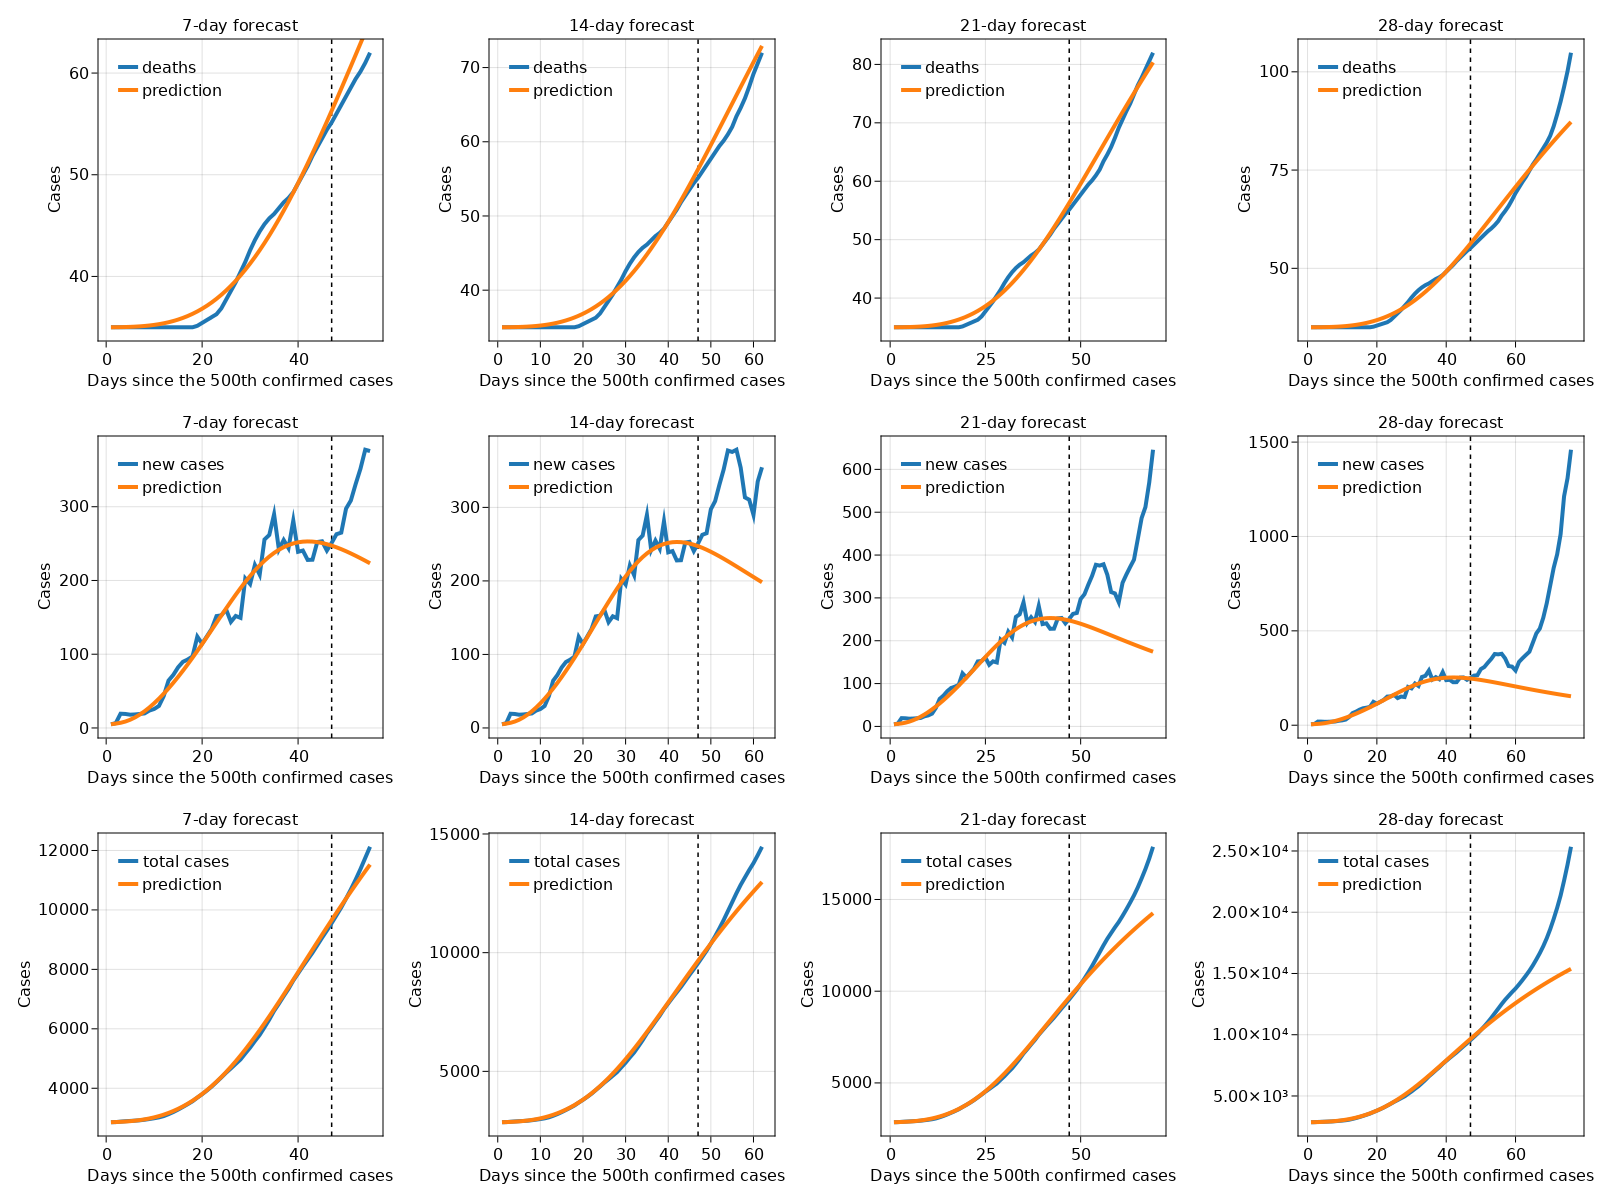
\includegraphics[scale=0.25]{baseline/vietnam/20211216111951.baseline.vietnam.forecasts.png}
    \caption{Predictions made by the baseline model after having trained with data for Vietnam. The black vertical dashed line marks the last day in the training period.}
    \label{fig:predictions-vietnam-baseline}
\end{figure}

\begin{figure}[!htb]
    \centering
    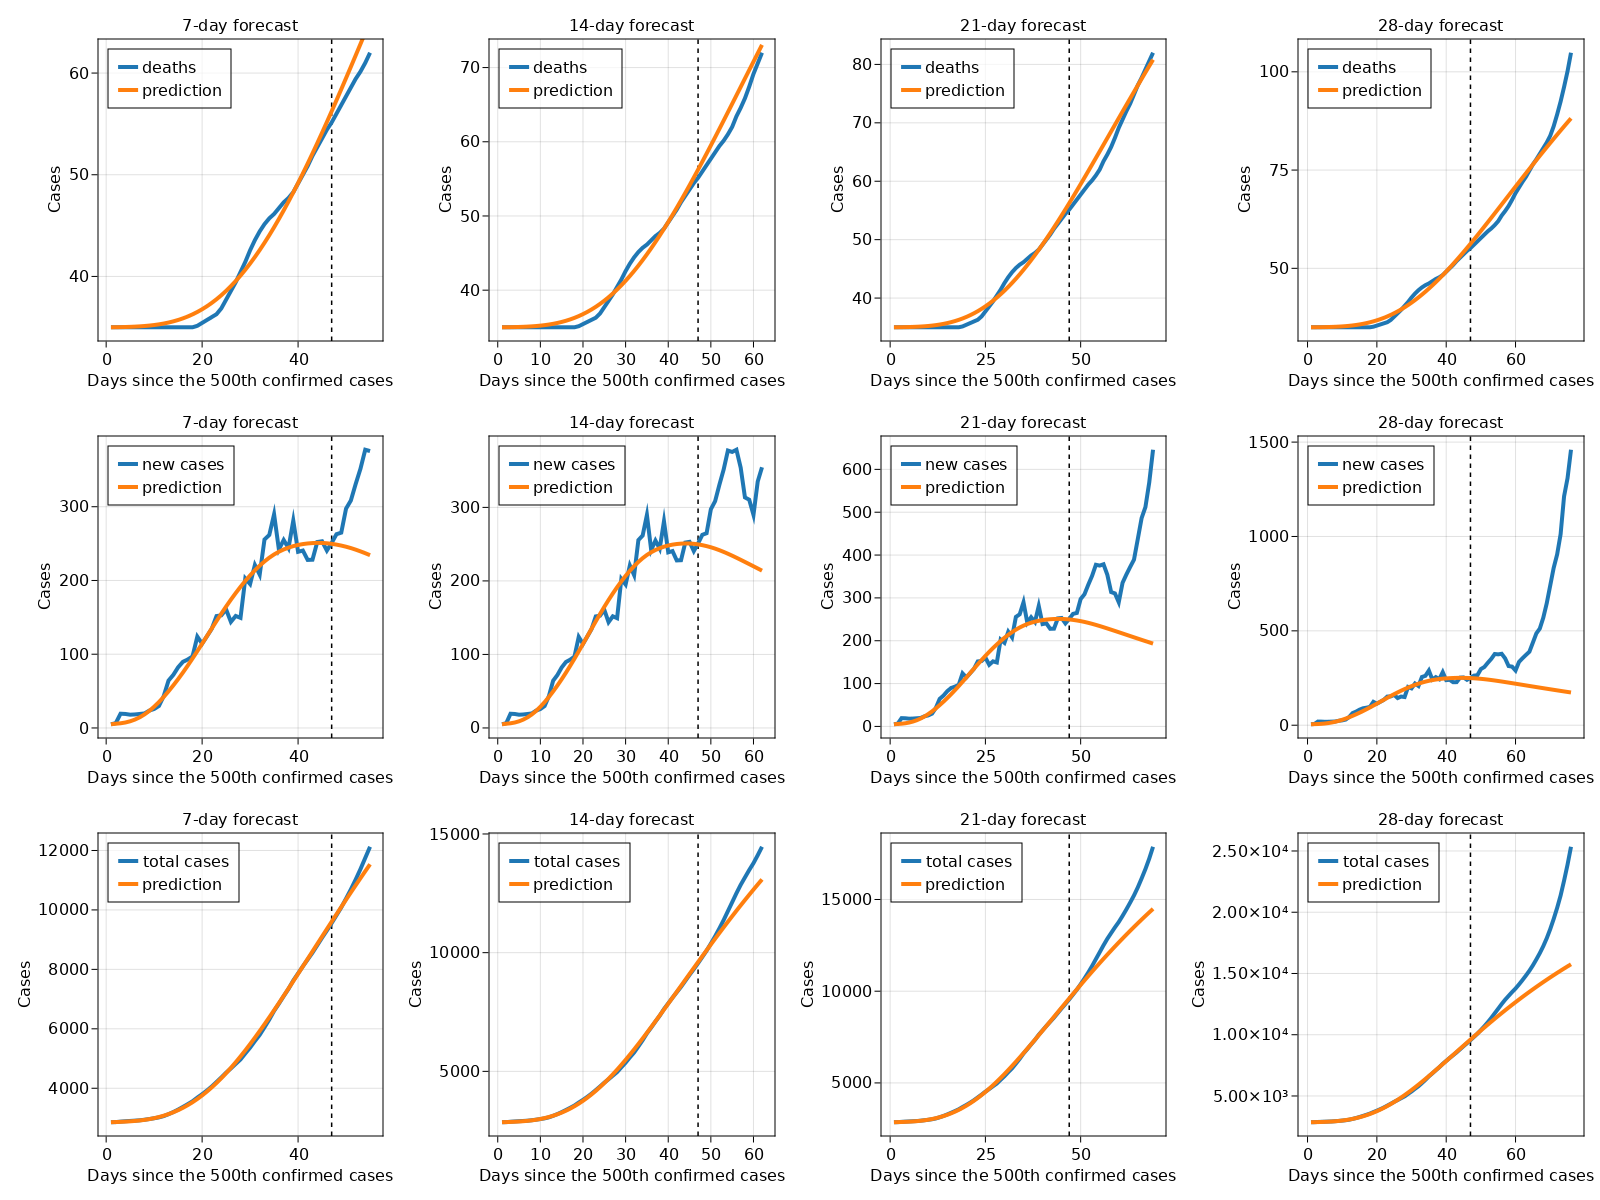
\includegraphics[scale=0.25]{fb1/vietnam/20211216231719.fbmobility1.vietnam.forecasts.png}
    \caption{Predictions made by the second version of the model that uses Facebook's Movement Range Maps dataset after having trained with data for Vietnam. The black vertical dashed line marks the last day in the training period.}
    \label{fig:predictions-vietnam-fb1}
\end{figure}

% US

\begin{figure}[!htb]
    \centering
    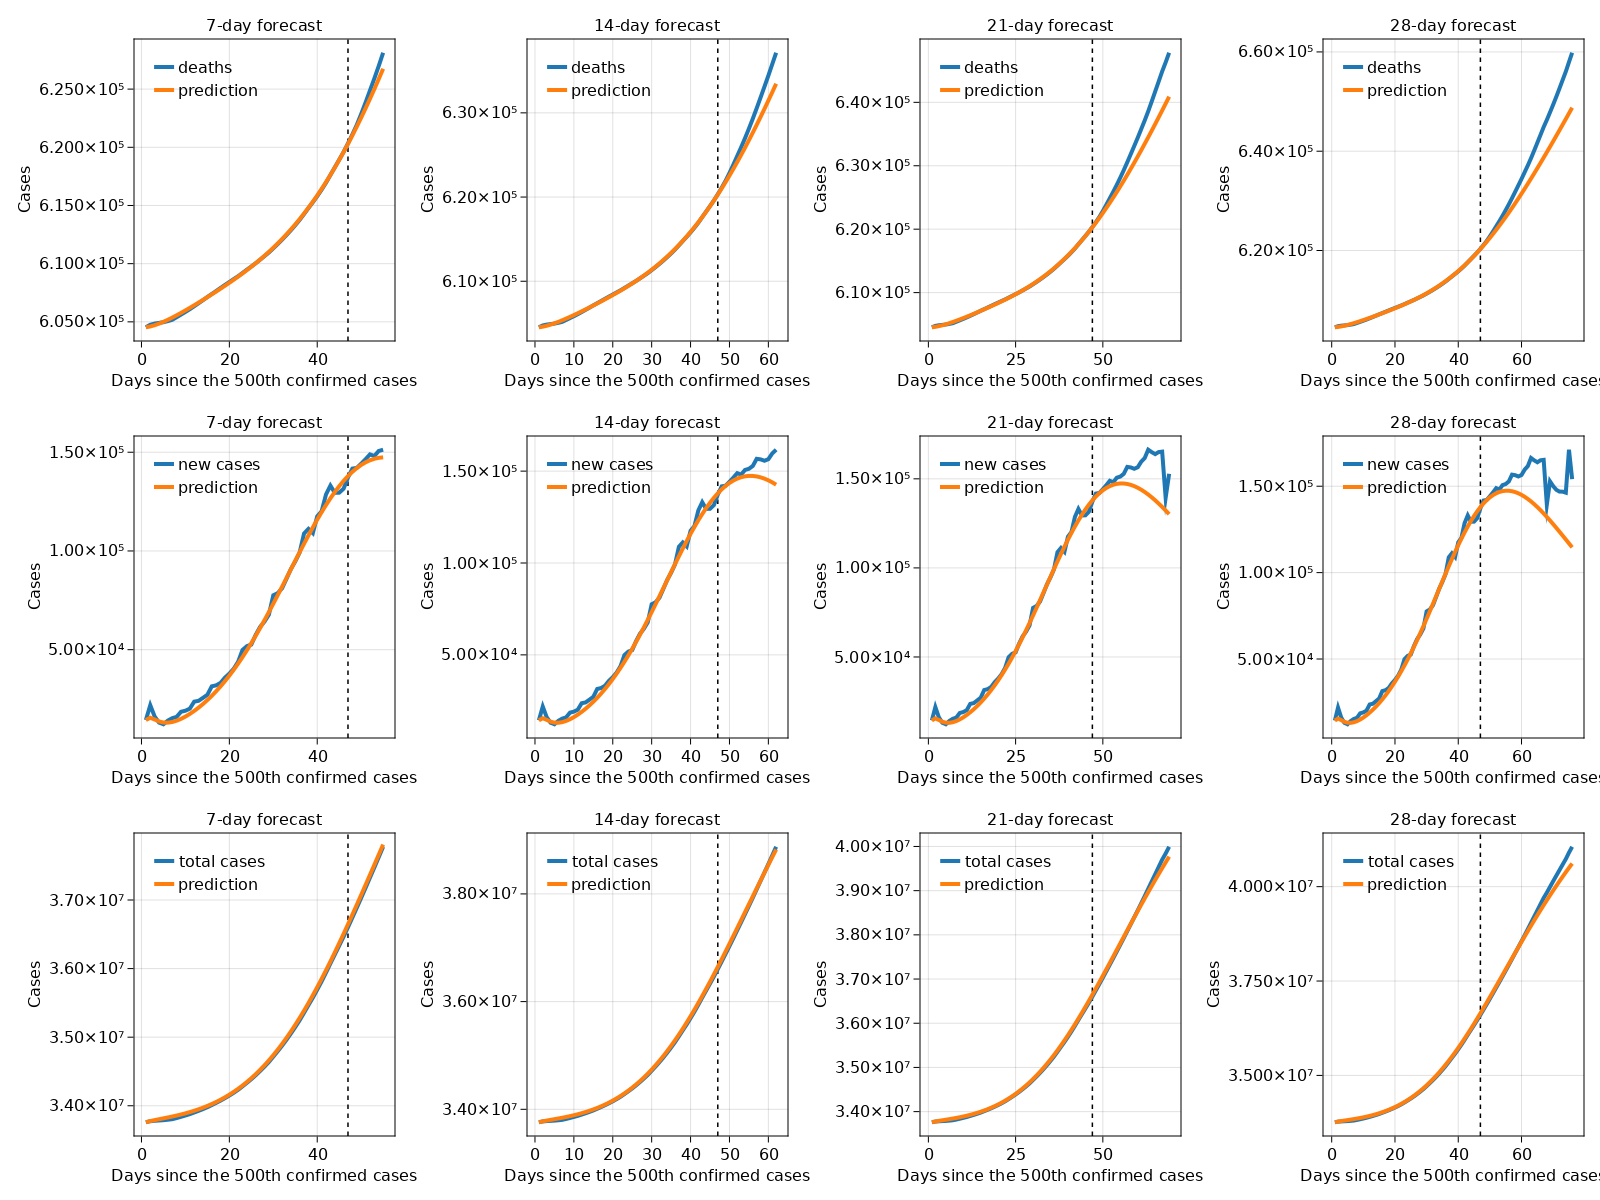
\includegraphics[scale=0.25]{baseline/unitedstates/20211216125000.baseline.unitedstates.forecasts.png}
    \caption{Predictions made by the baseline model after having trained with data for the United States. The black vertical dashed line marks the last day in the training period.}
    \label{fig:predictions-usa-baseline}
\end{figure}

\begin{figure}[!htb]
    \centering
    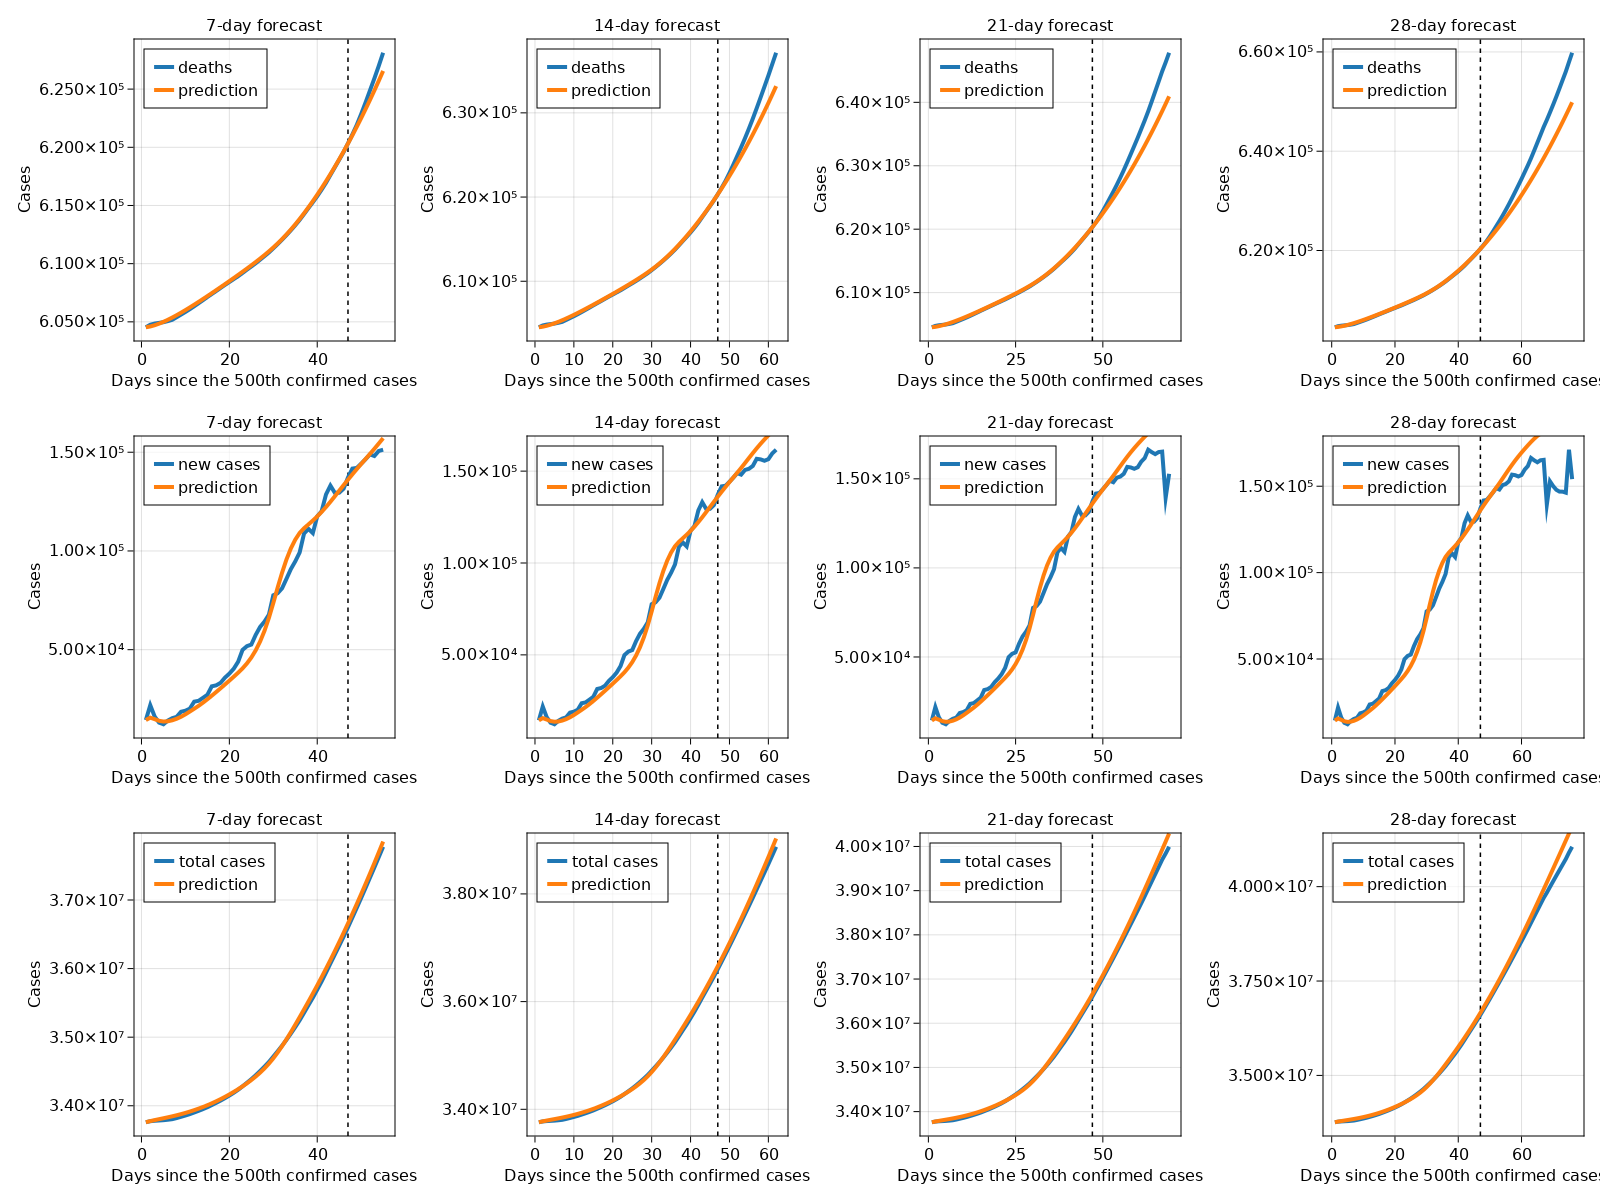
\includegraphics[scale=0.25]{fb1/unitedstates/20211216233634.fbmobility1.unitedstates.forecasts.png}
    \caption{Predictions made by the second version of the model that uses Facebook's Movement Range Maps dataset after having trained with data for the United States. The black vertical dashed line marks the last day in the training period.}
    \label{fig:predictions-usa-fb1}
\end{figure}

% LOS ANGELES

\begin{figure}[!htb]
    \centering
    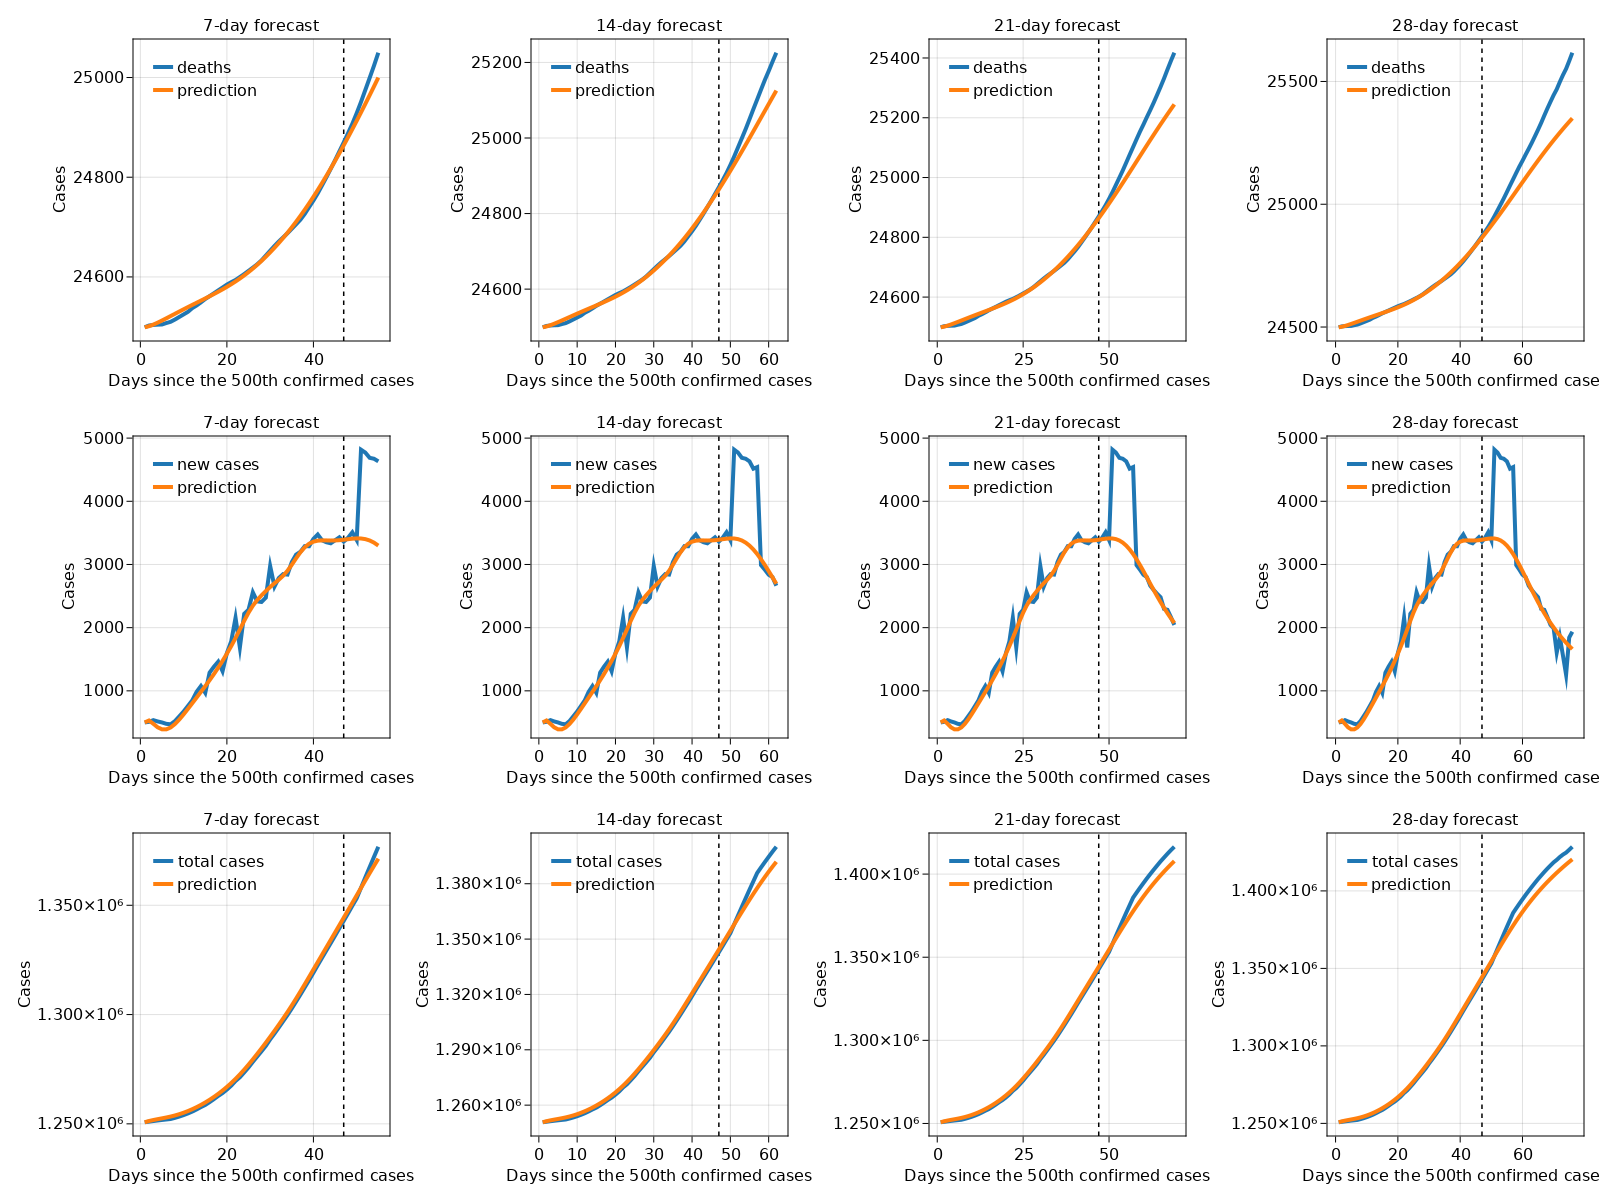
\includegraphics[scale=0.25]{baseline/losangeles_ca/20211216124108.baseline.losangeles_ca.forecasts.png}
    \caption{Predictions made by the baseline model after having trained with data for Los Angeles, California. The black vertical dashed line marks the last day in the training period.}
    \label{fig:predictions-losangeles-baseline}
\end{figure}

\begin{figure}[!htb]
    \centering
    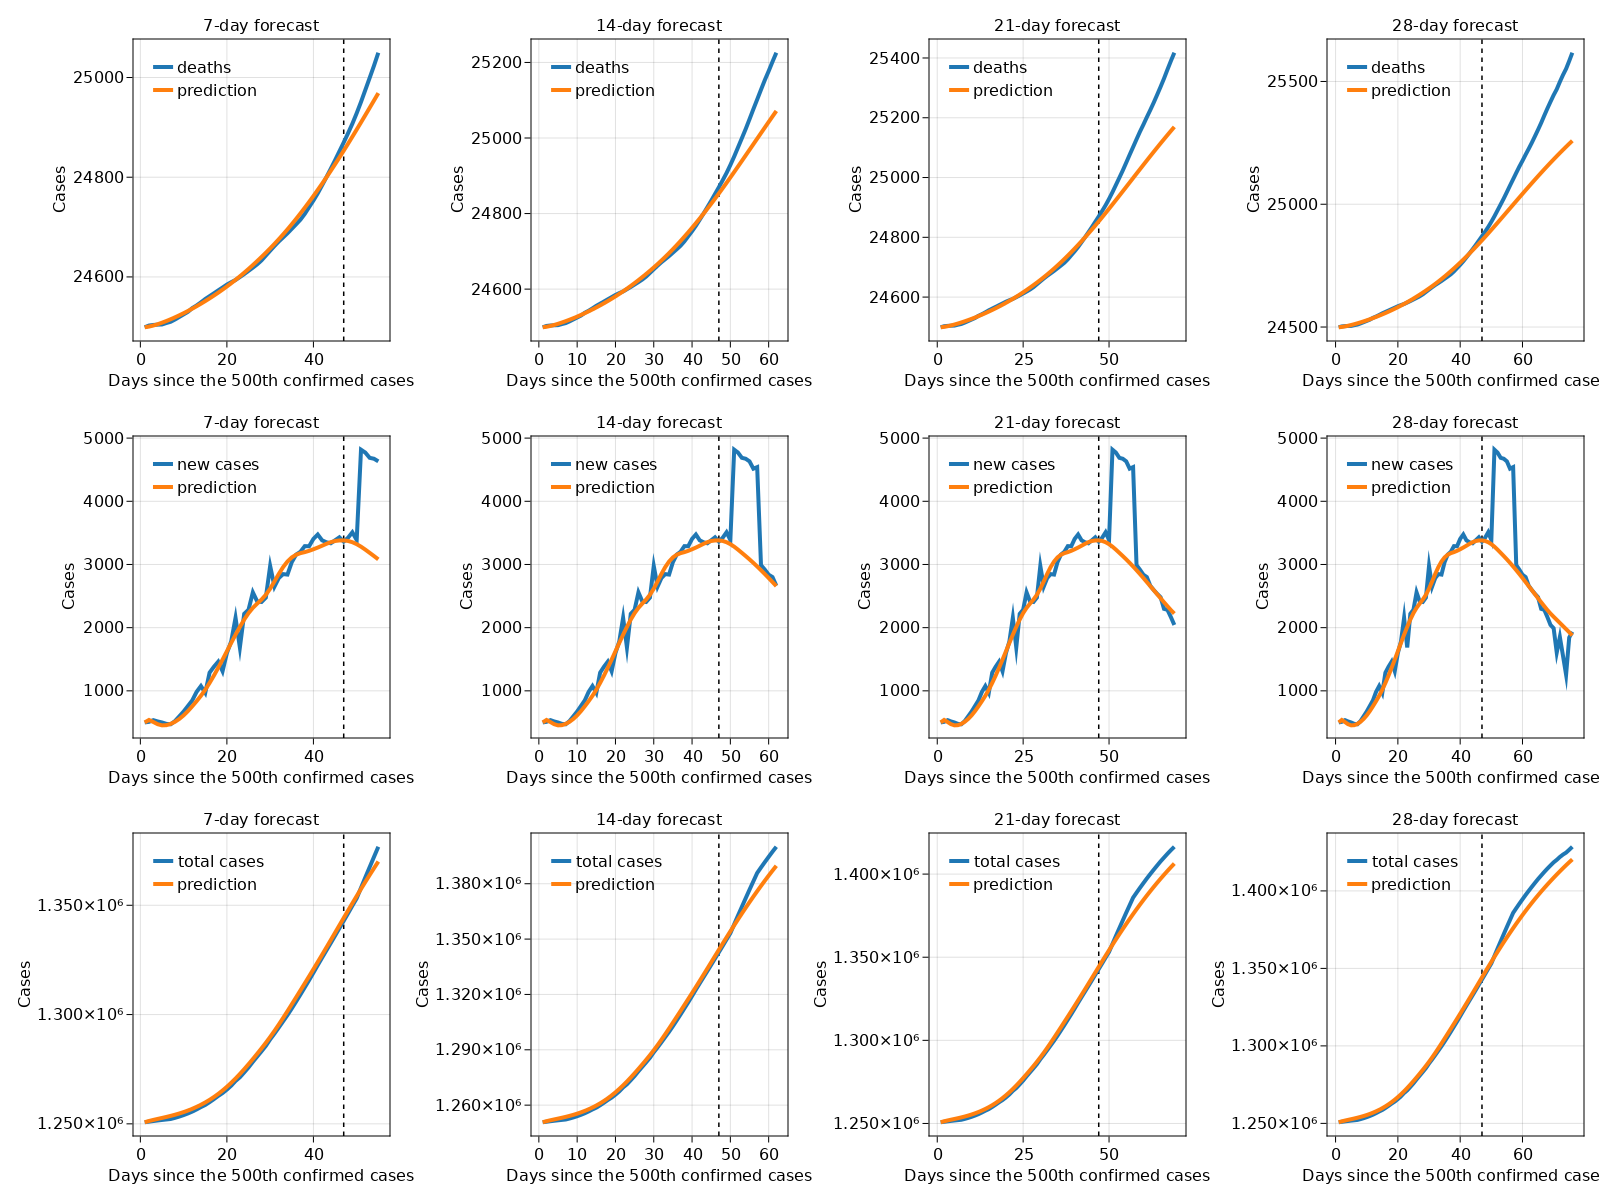
\includegraphics[scale=0.25]{fb1/losangeles_ca/20211216180602.fbmobility1.losangeles_ca.forecasts.png}
    \caption{Predictions made by the second version of the model that uses Facebook's Movement Range Maps dataset after having trained with data for Los Angeles, California. The black vertical dashed line marks the last day in the training period.}
    \label{fig:predictions-losangeles-fb1}
\end{figure}

\begin{figure}[!htb]
    \centering
    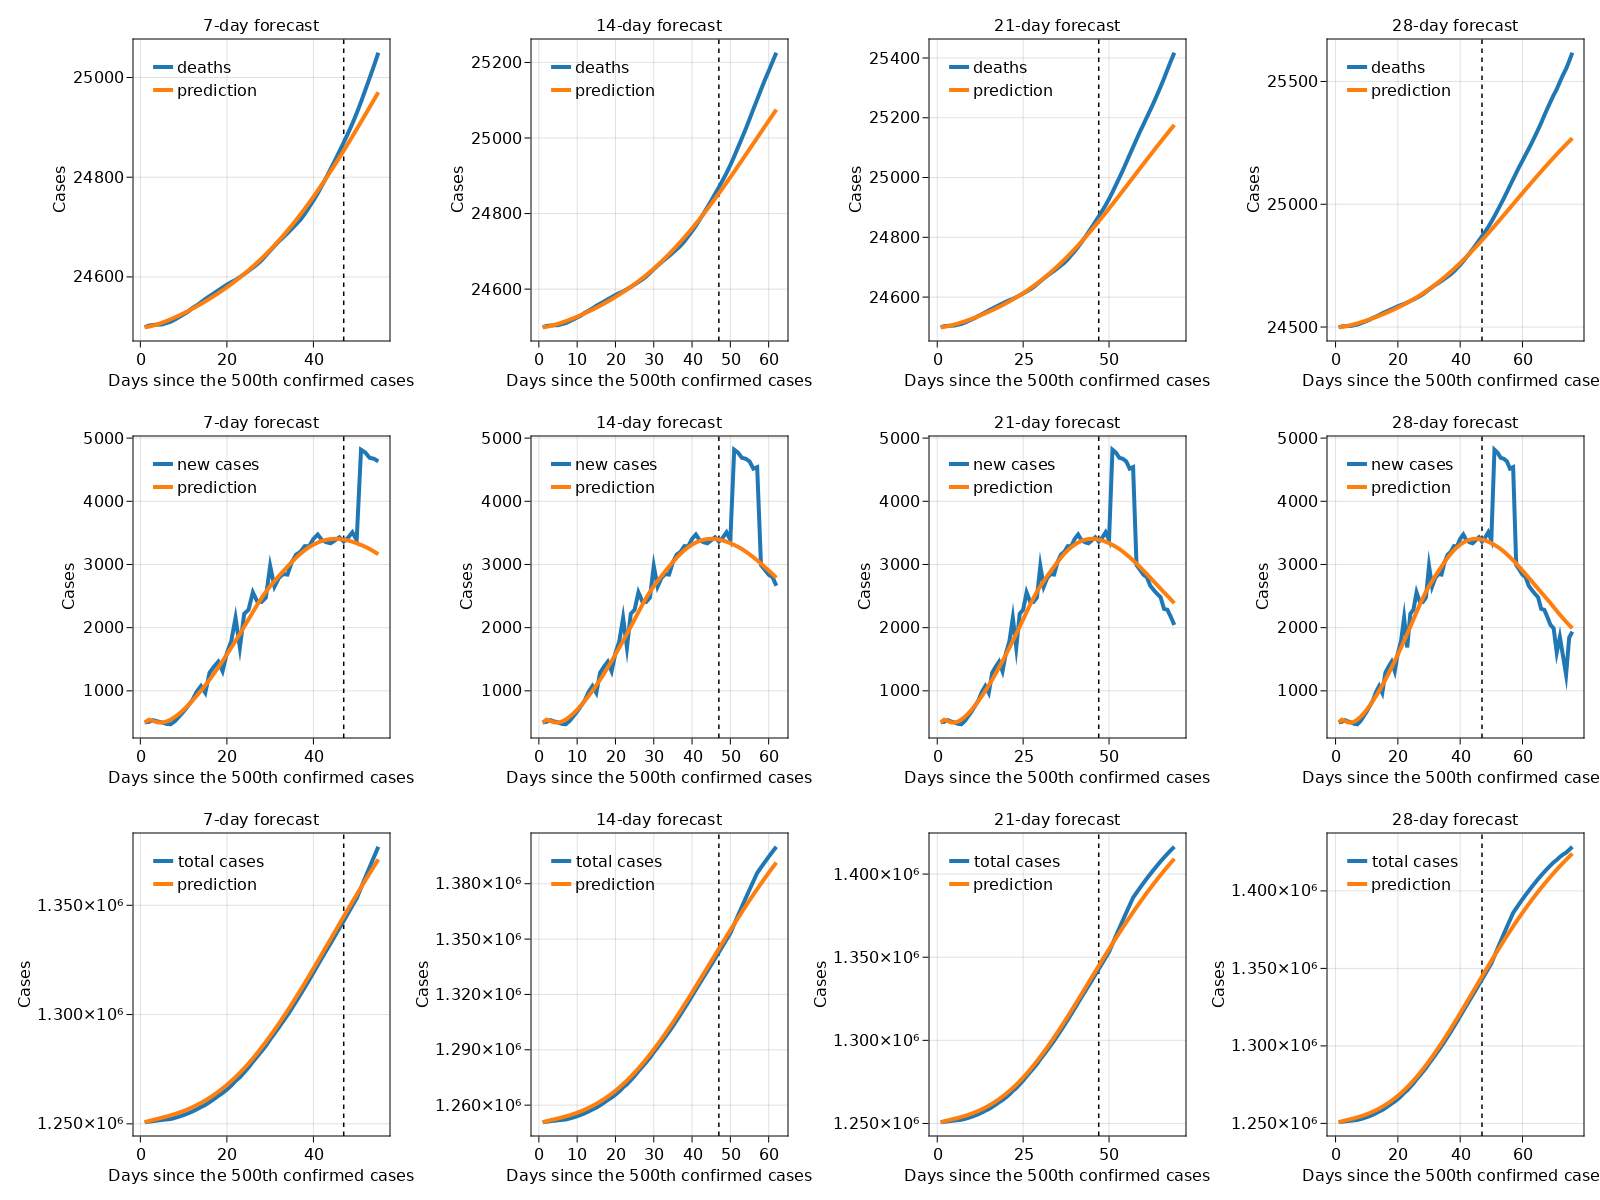
\includegraphics[scale=0.25]{fb2/losangeles_ca/20211216142727.fbmobility2.losangeles_ca.forecasts.png}
    \caption{Predictions made by the second version of the model that uses Facebook's Movement Range Maps dataset and Social Proximity to Cases Index after having trained with data for Los Angeles, California. The black vertical dashed line marks the last day in the training period.}
    \label{fig:predictions-losangeles-fb2}
\end{figure}

% HARRIS

\begin{figure}[!htb]
    \centering
    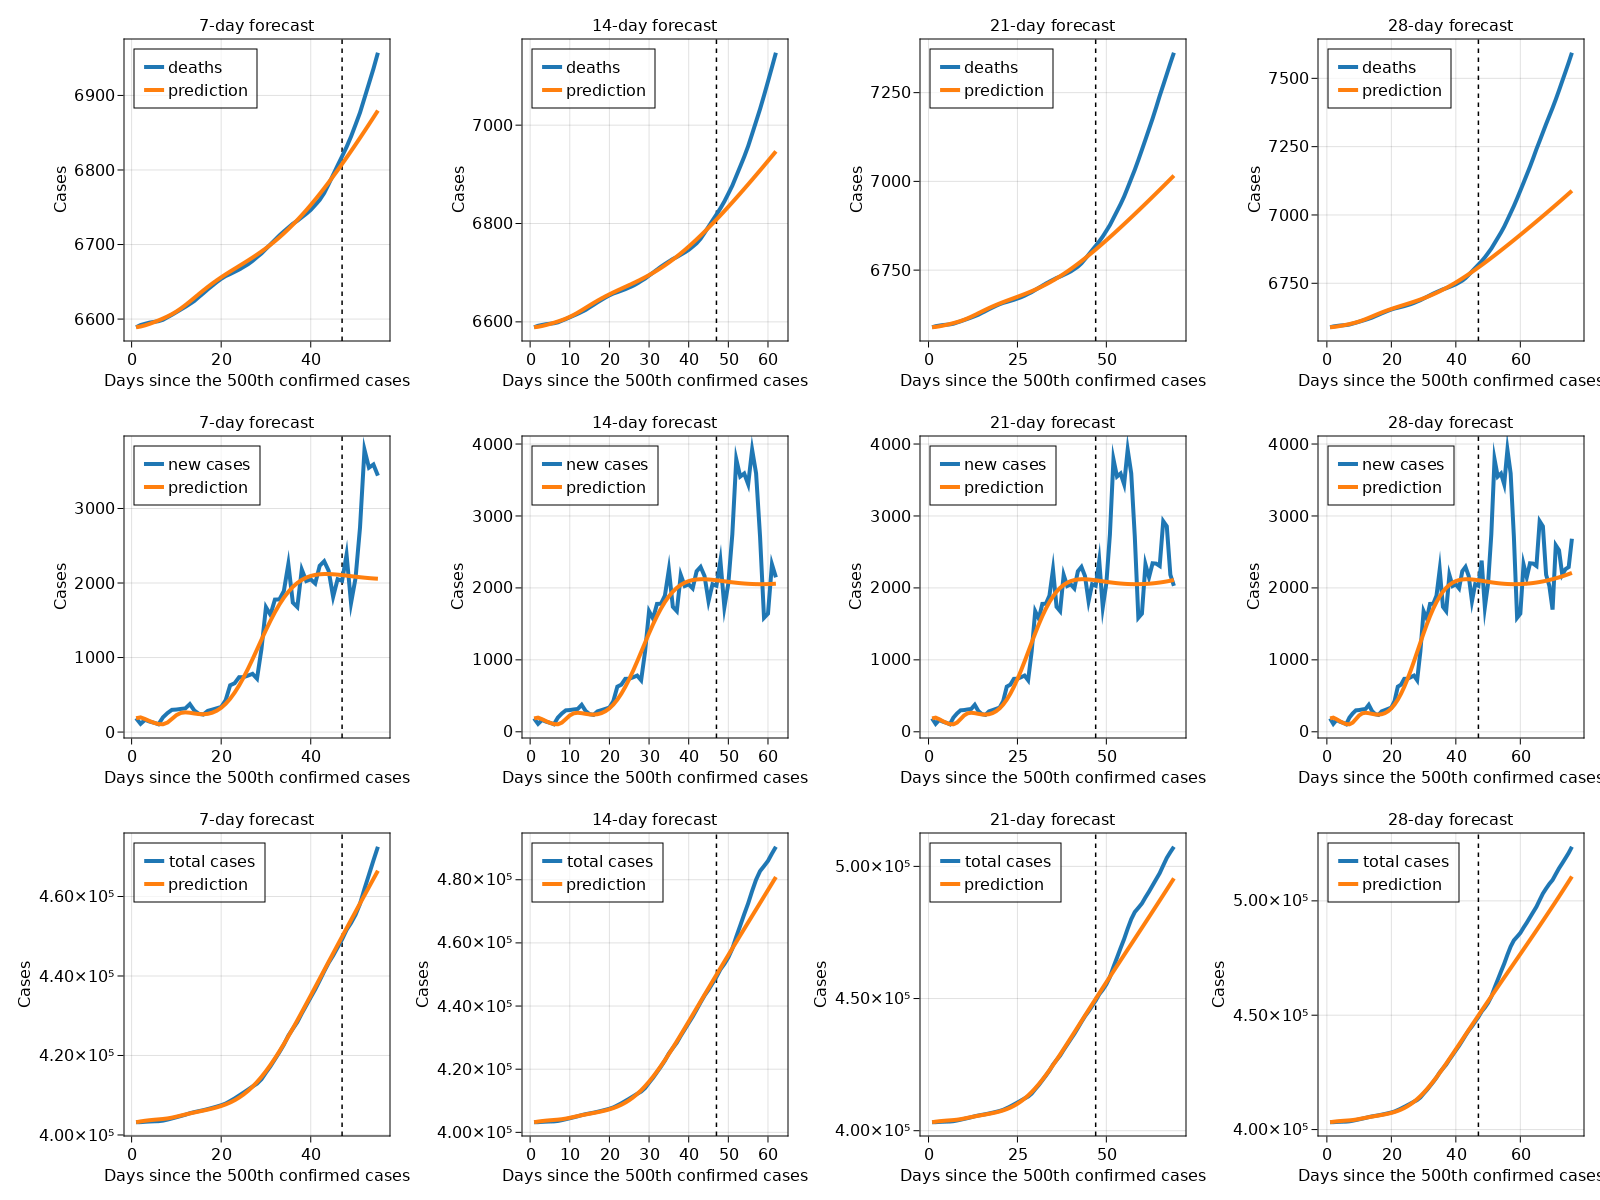
\includegraphics[scale=0.25]{baseline/harris_tx/20211216154445.baseline.harris_tx.forecasts.png}
    \caption{Predictions made by the baseline model after having trained with data for Harris, Texas. The black vertical dashed line marks the last day in the training period.}
    \label{fig:predictions-harris-baseline}
\end{figure}

\begin{figure}[!htb]
    \centering
    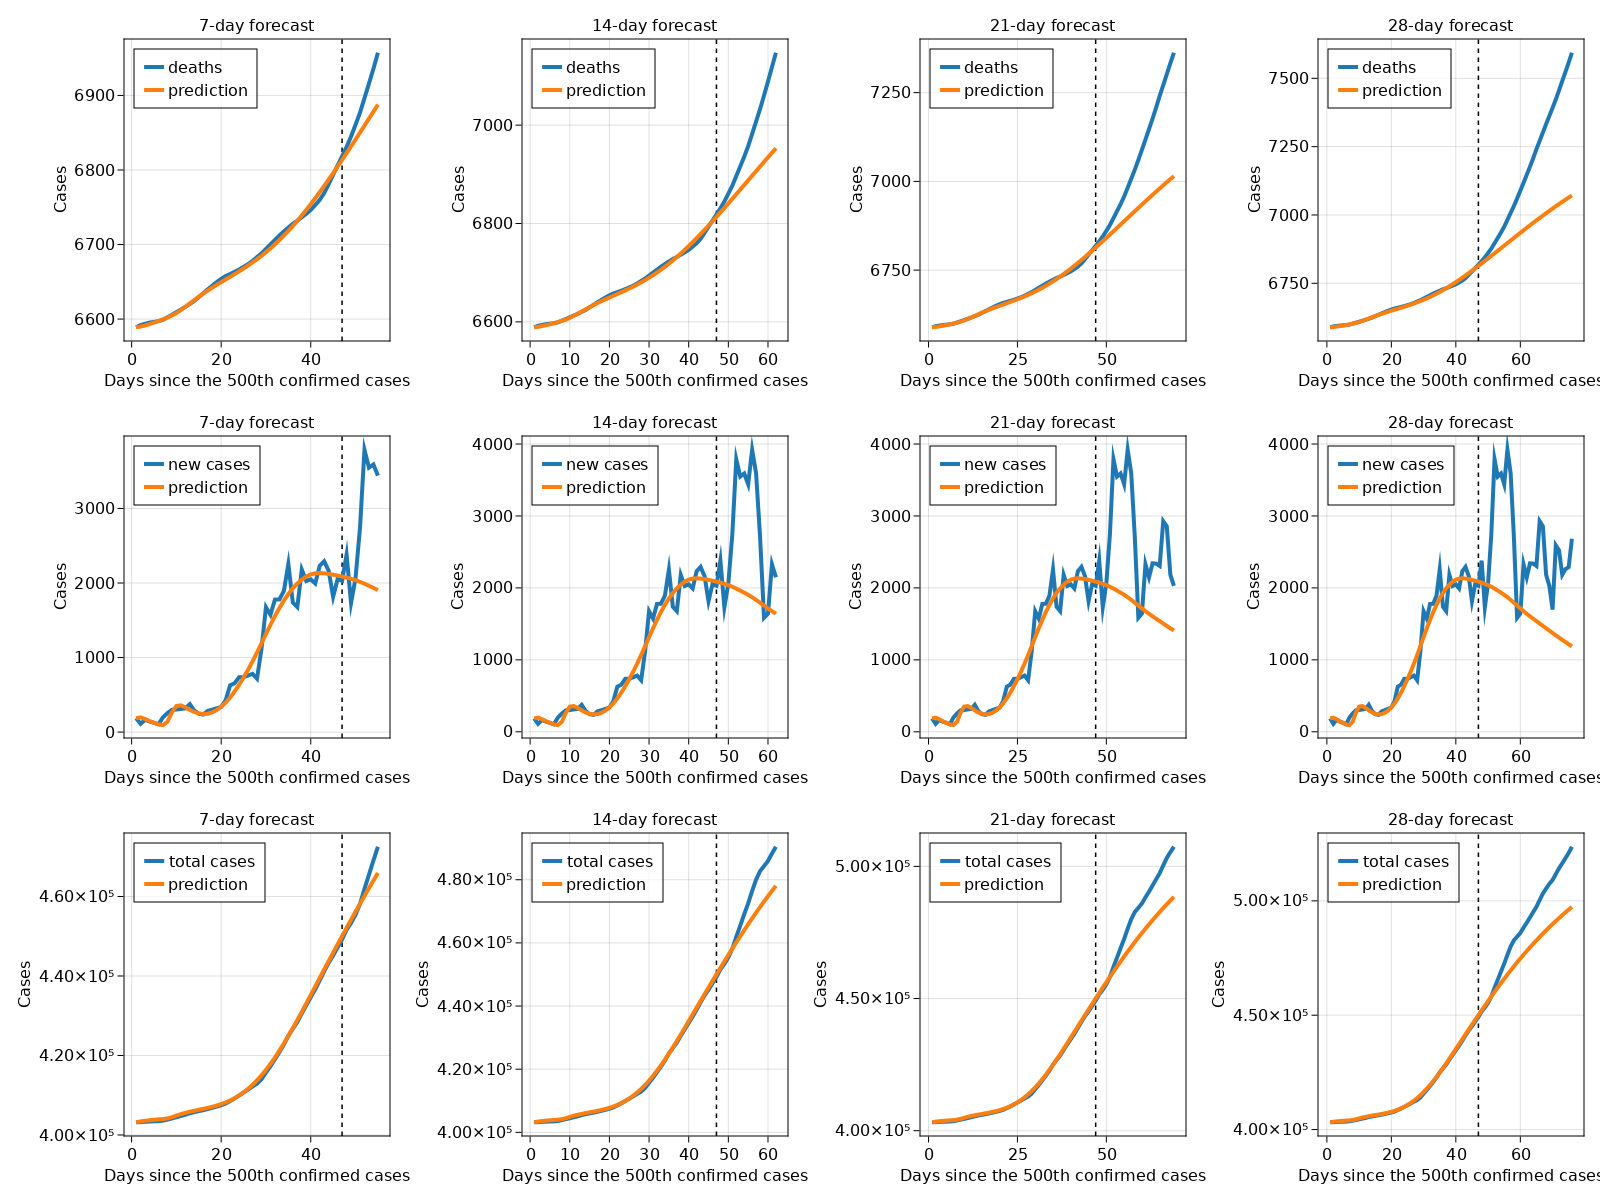
\includegraphics[scale=0.25]{fb1/harris_tx/20211216231719.fbmobility1.harris_tx.forecasts.png}
    \caption{Predictions made by the second version of the model that uses Facebook's Movement Range Maps dataset after having trained with data for Harris, Texas. The black vertical dashed line marks the last day in the training period.}
    \label{fig:predictions-harris-fb1}
\end{figure}

\begin{figure}[!htb]
    \centering
    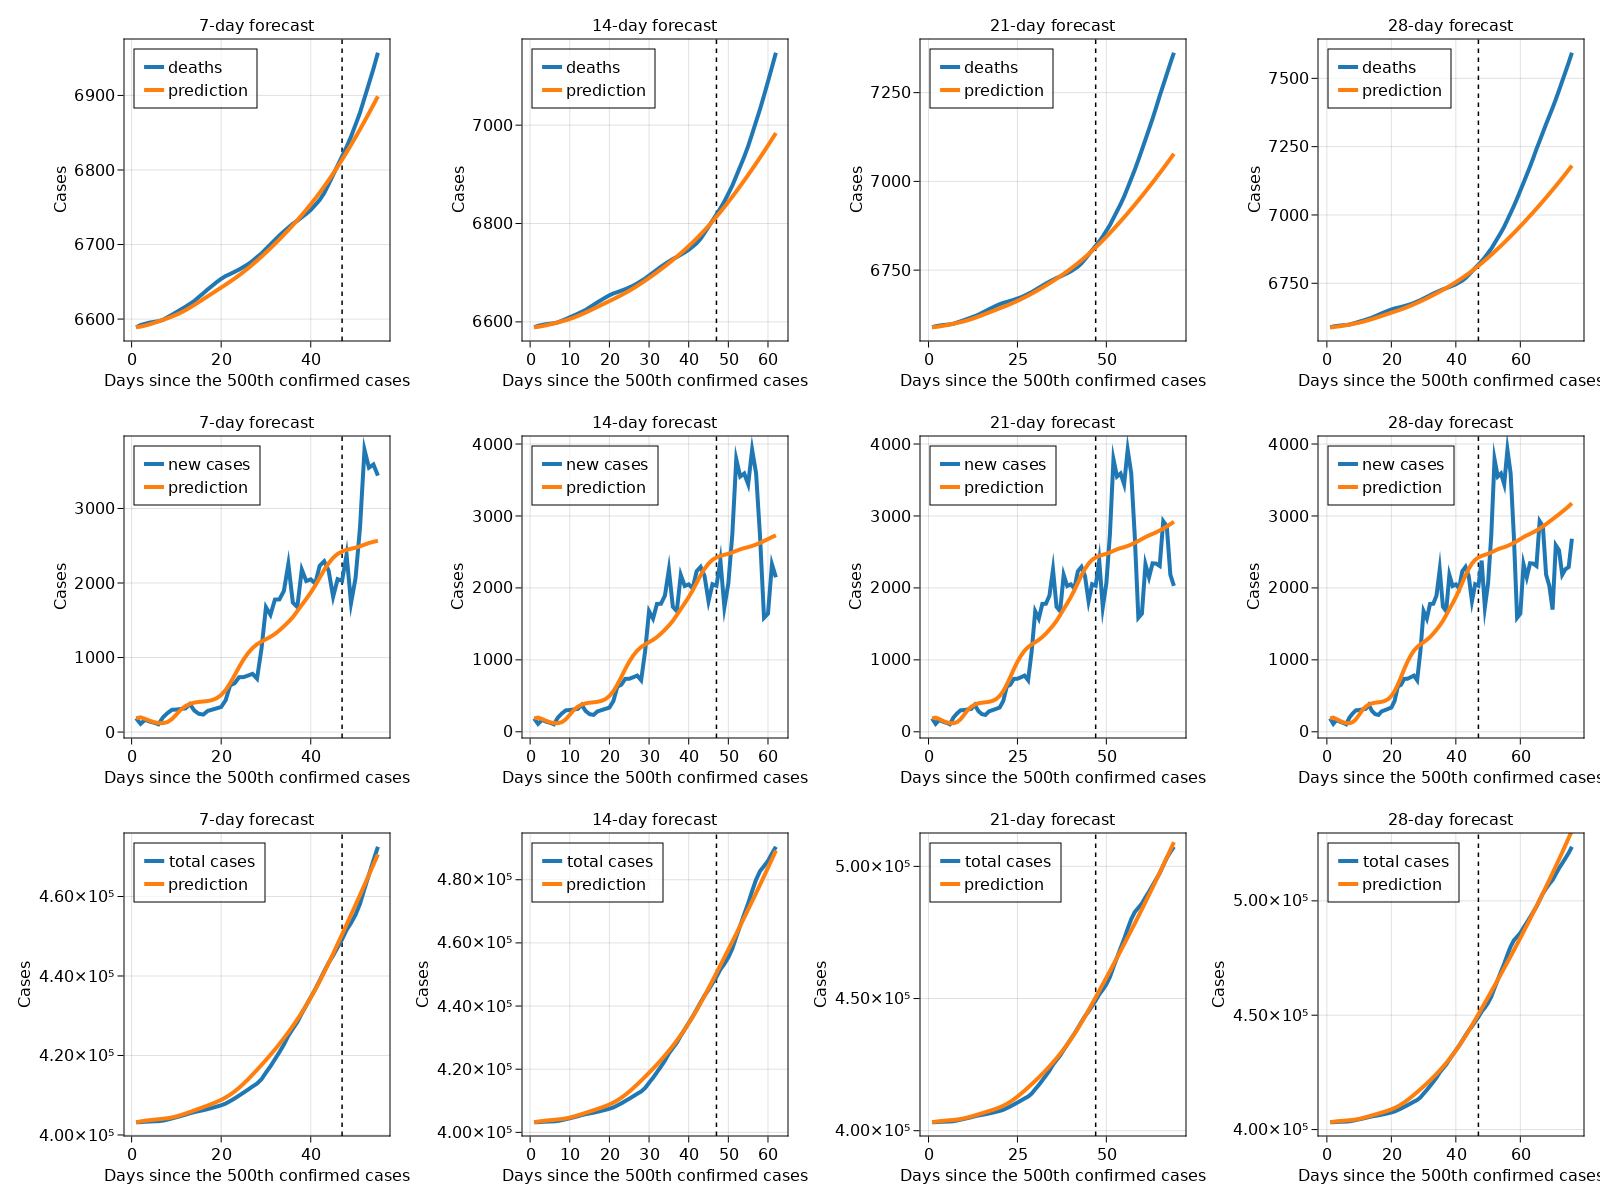
\includegraphics[scale=0.25]{fb2/harris_tx/20211217204936.fbmobility2.harris_tx.forecasts.png}
    \caption{Predictions made by the second version of the model that uses Facebook's Movement Range Maps dataset and Social Proximity to Cases Index after having trained with data for Harris, Texas. The black vertical dashed line marks the last day in the training period.}
    \label{fig:predictions-harris-fb2}
\end{figure}

% COOK

\begin{figure}[!htb]
    \centering
    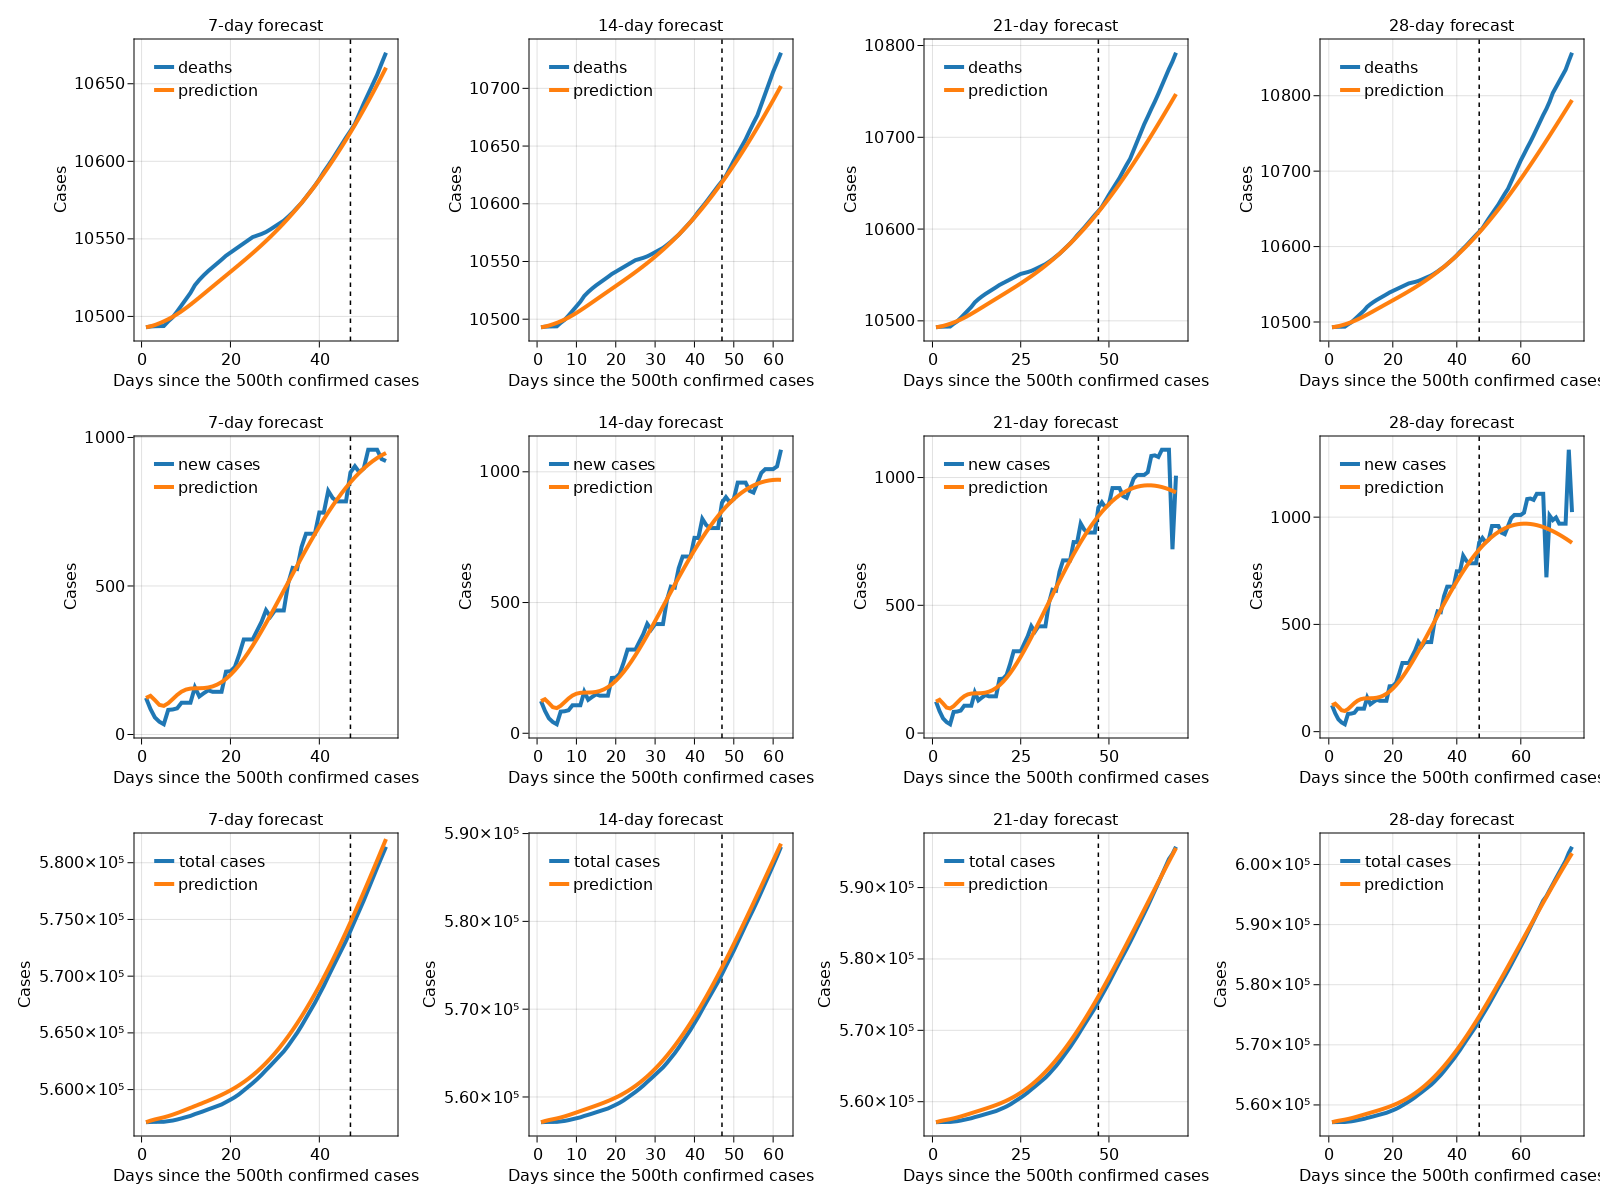
\includegraphics[scale=0.25]{baseline/cook_il/20211215163025.baseline.cook_il.forecasts.png}
    \caption{Predictions made by the baseline model after having trained with data for Cook, Illinois. The black vertical dashed line marks the last day in the training period.}
    \label{fig:predictions-cook-baseline}
\end{figure}

\begin{figure}[!htb]
    \centering
    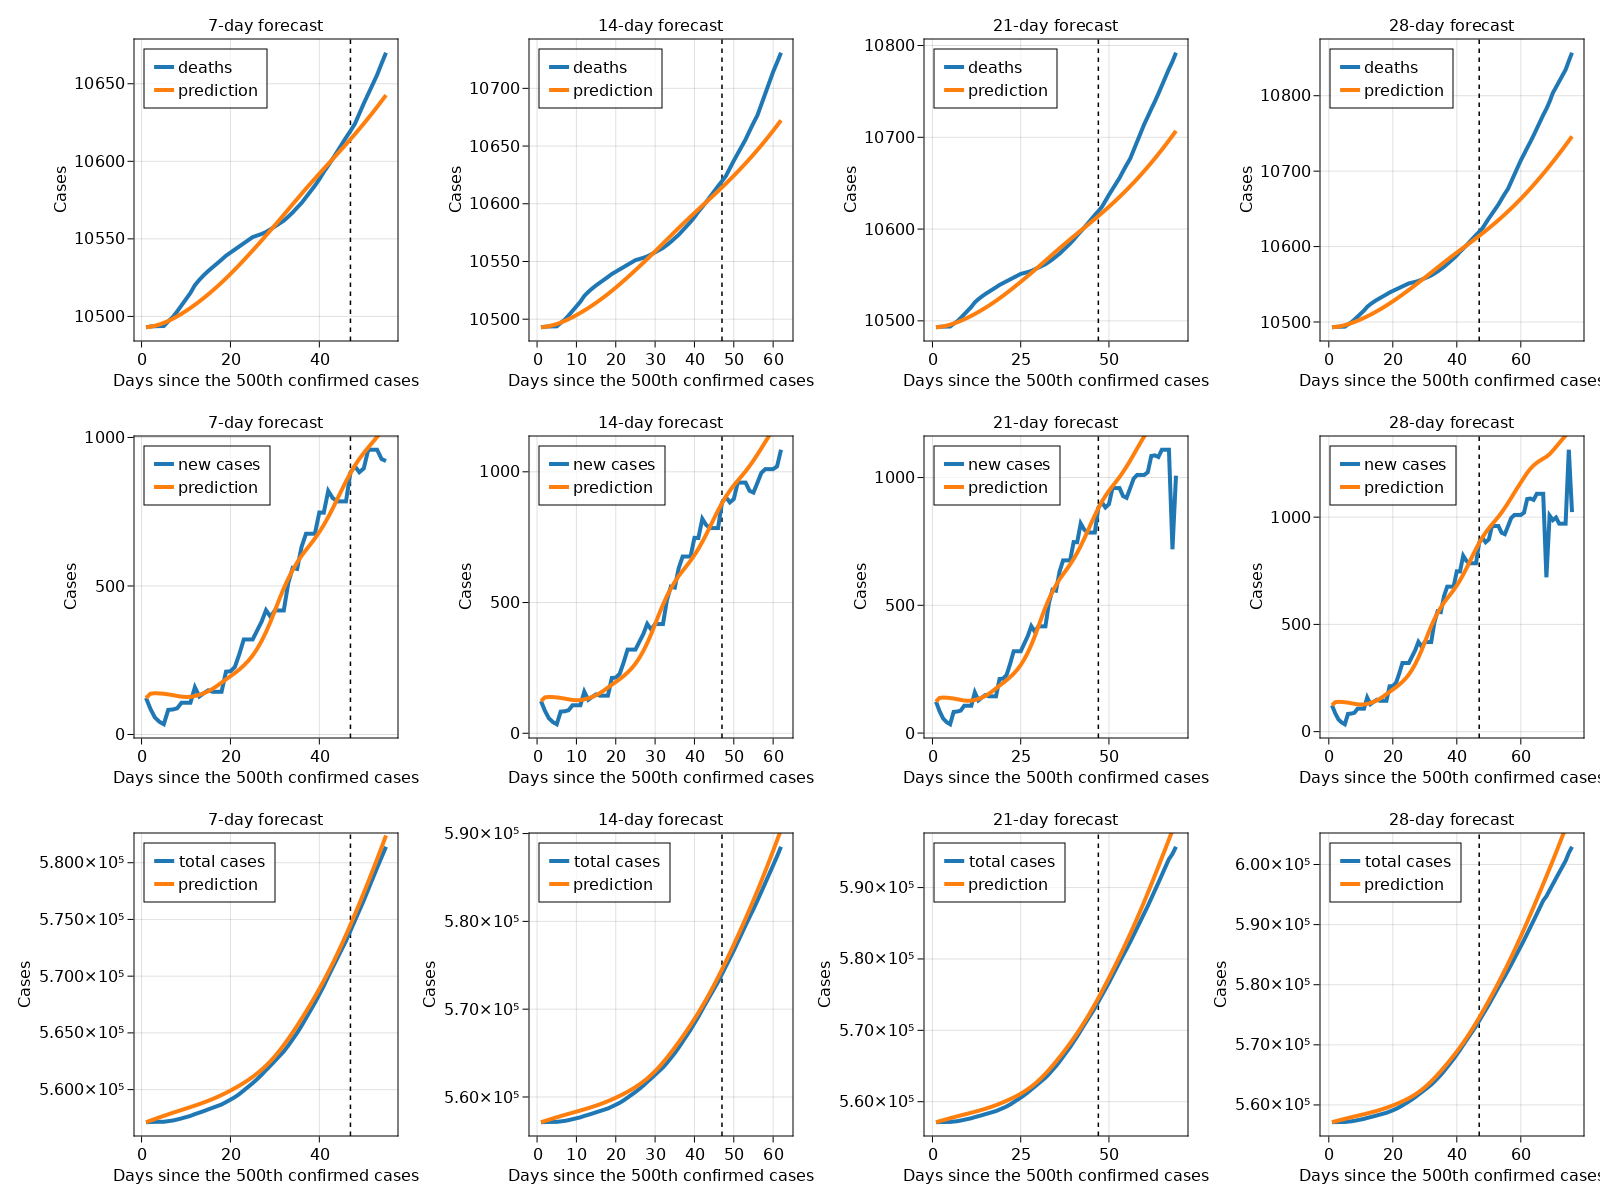
\includegraphics[scale=0.25]{fb1/cook_il/20211216131821.fbmobility1.cook_il.forecasts.png}
    \caption{Predictions made by the second version of the model that uses Facebook's Movement Range Maps dataset after having trained with data for Cook, Illinois. The black vertical dashed line marks the last day in the training period.}
    \label{fig:predictions-cook-fb1}
\end{figure}

\begin{figure}[!htb]
    \centering
    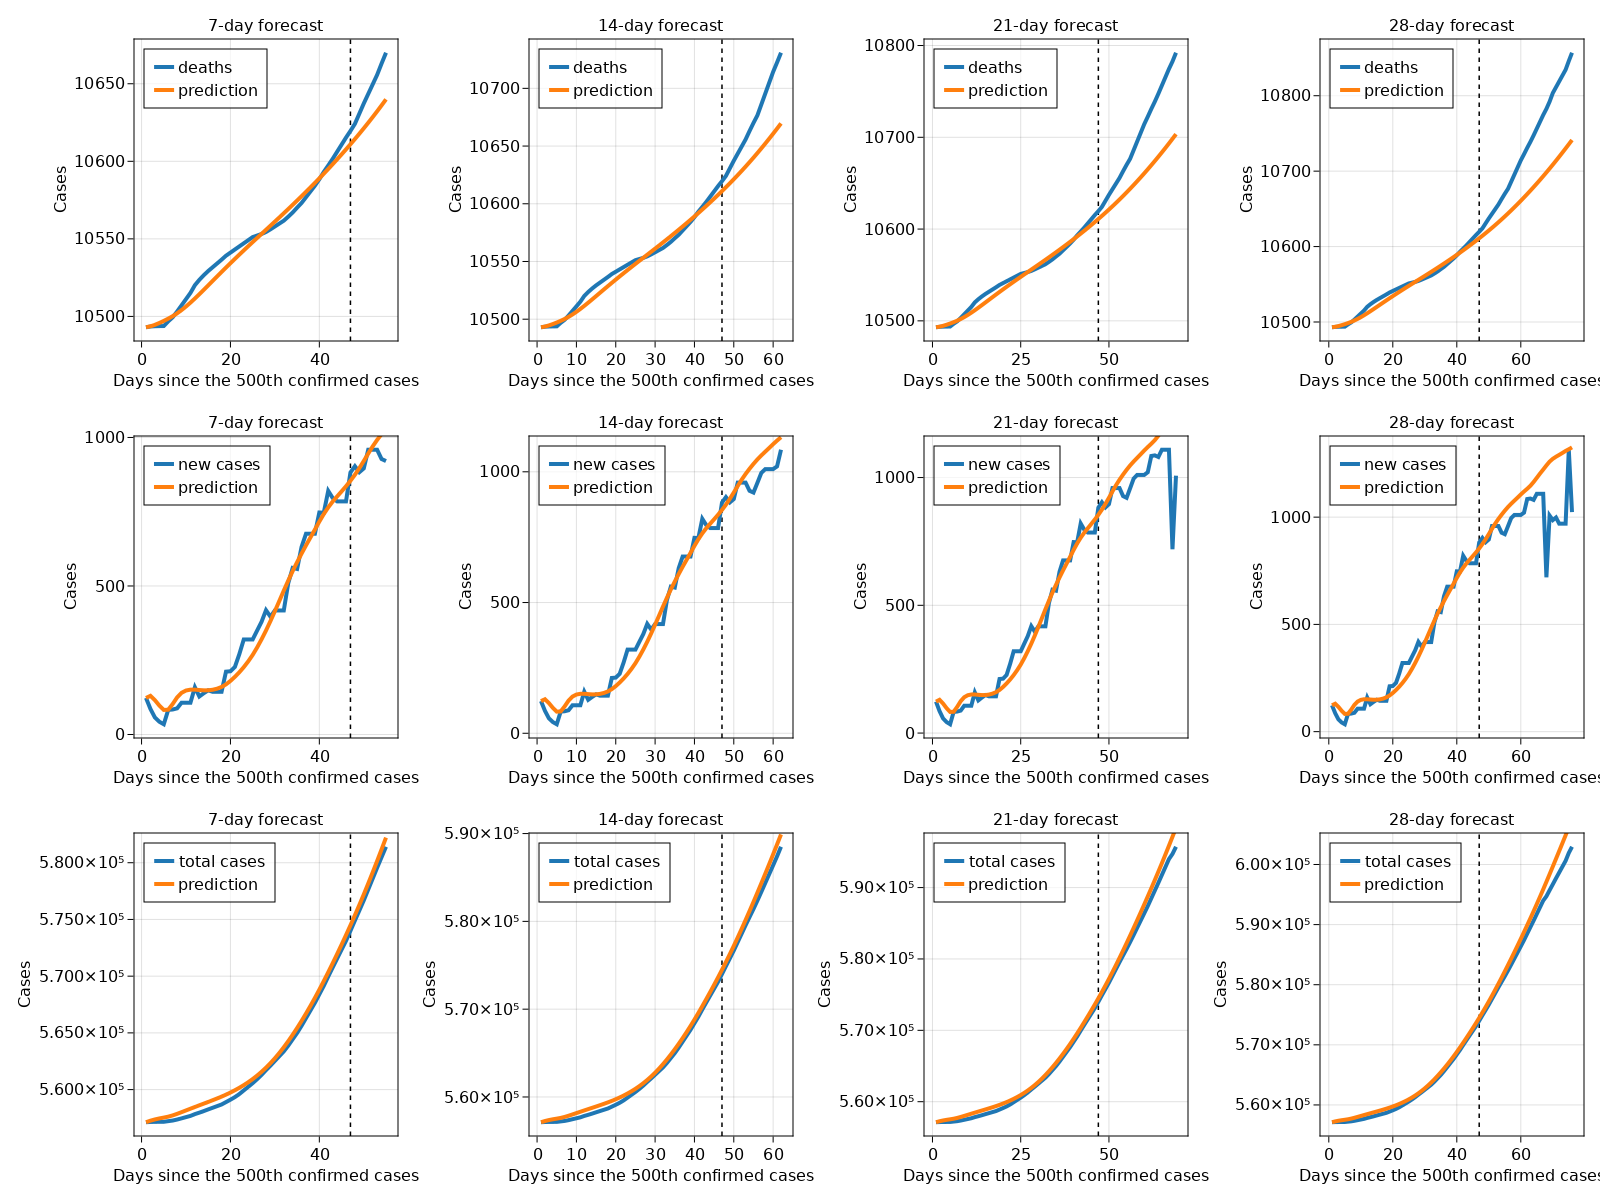
\includegraphics[scale=0.25]{fb2/cook_il/20211216142727.fbmobility2.cook_il.forecasts.png}
    \caption{Predictions made by the second version of the model that uses Facebook's Movement Range Maps dataset and Social Proximity to Cases Index after having trained with data for Cook, Illinois. The black vertical dashed line marks the last day in the training period.}
    \label{fig:predictions-cook-fb2}
\end{figure}

% MARICOPA

\begin{figure}[!htb]
    \centering
    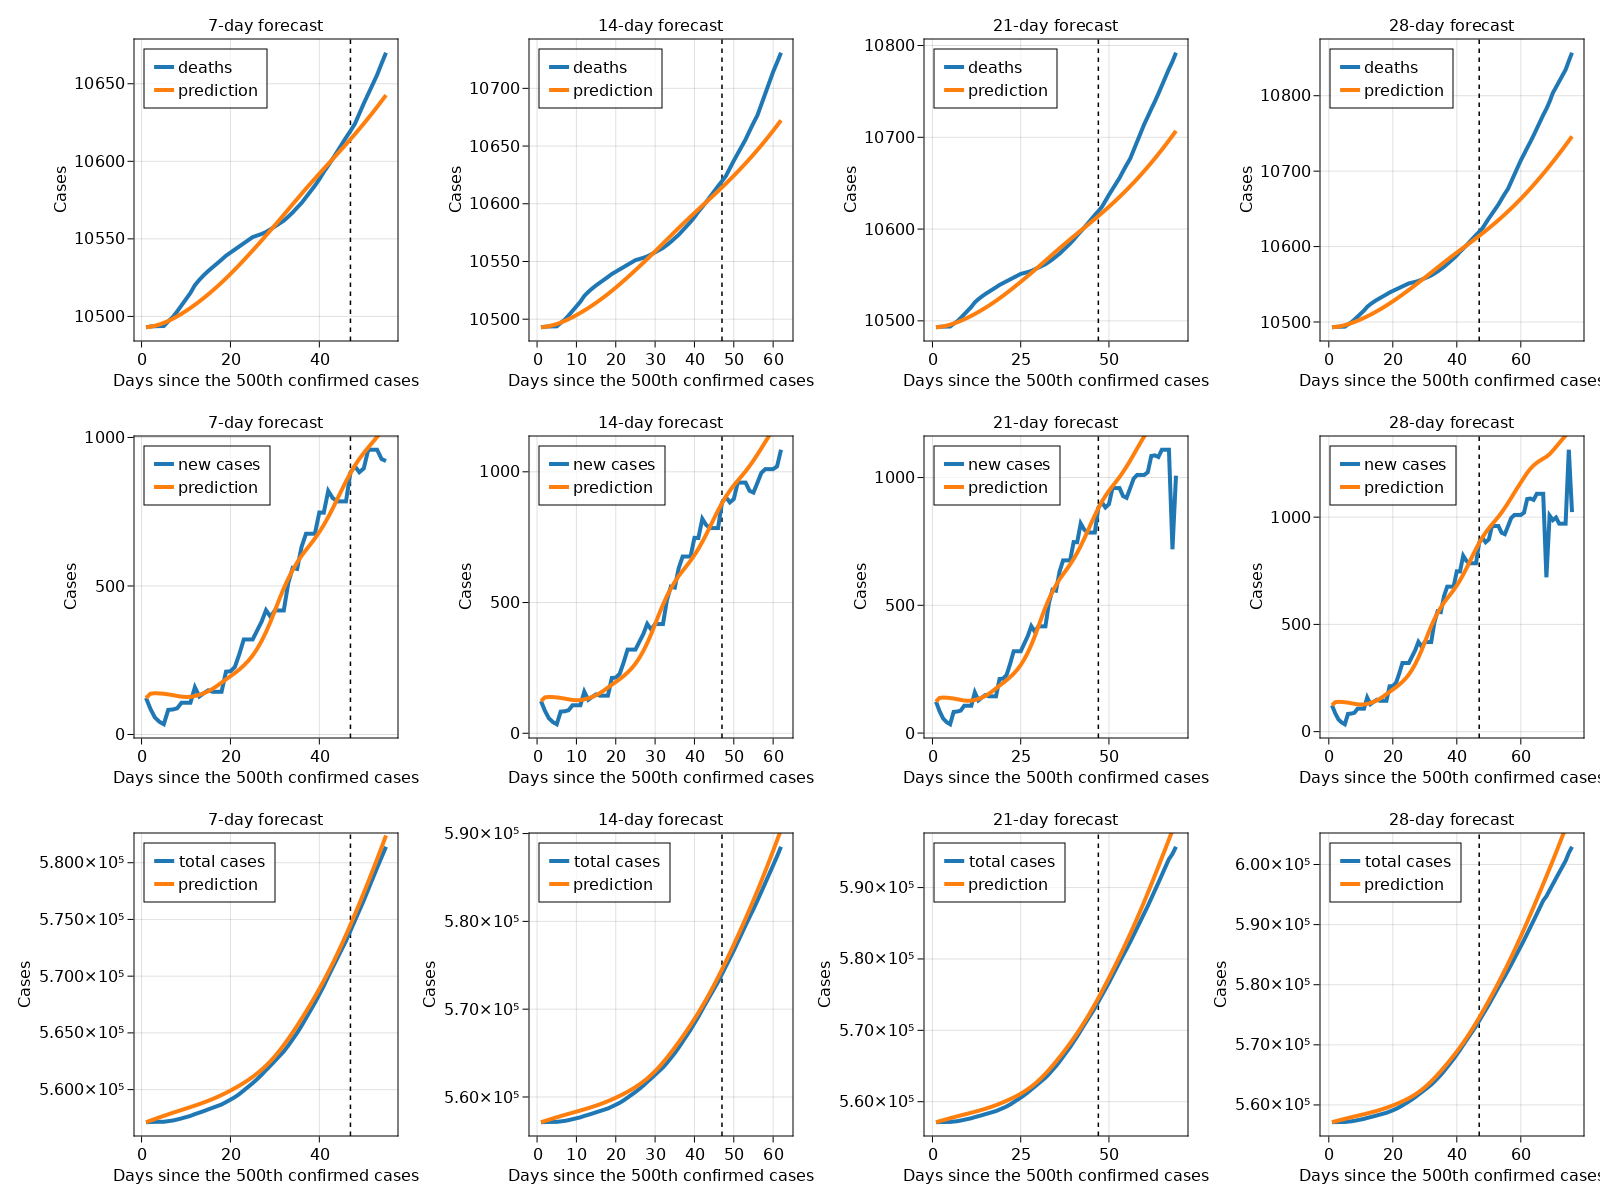
\includegraphics[scale=0.25]{fb1/cook_il/20211216131821.fbmobility1.cook_il.forecasts.png}
    \caption{Predictions made by the baseline model after having trained with data for Maricopa, Arizona. The black vertical dashed line marks the last day in the training period.}
    \label{fig:predictions-maricopa-baseline}
\end{figure}

\begin{figure}[!htb]
    \centering
    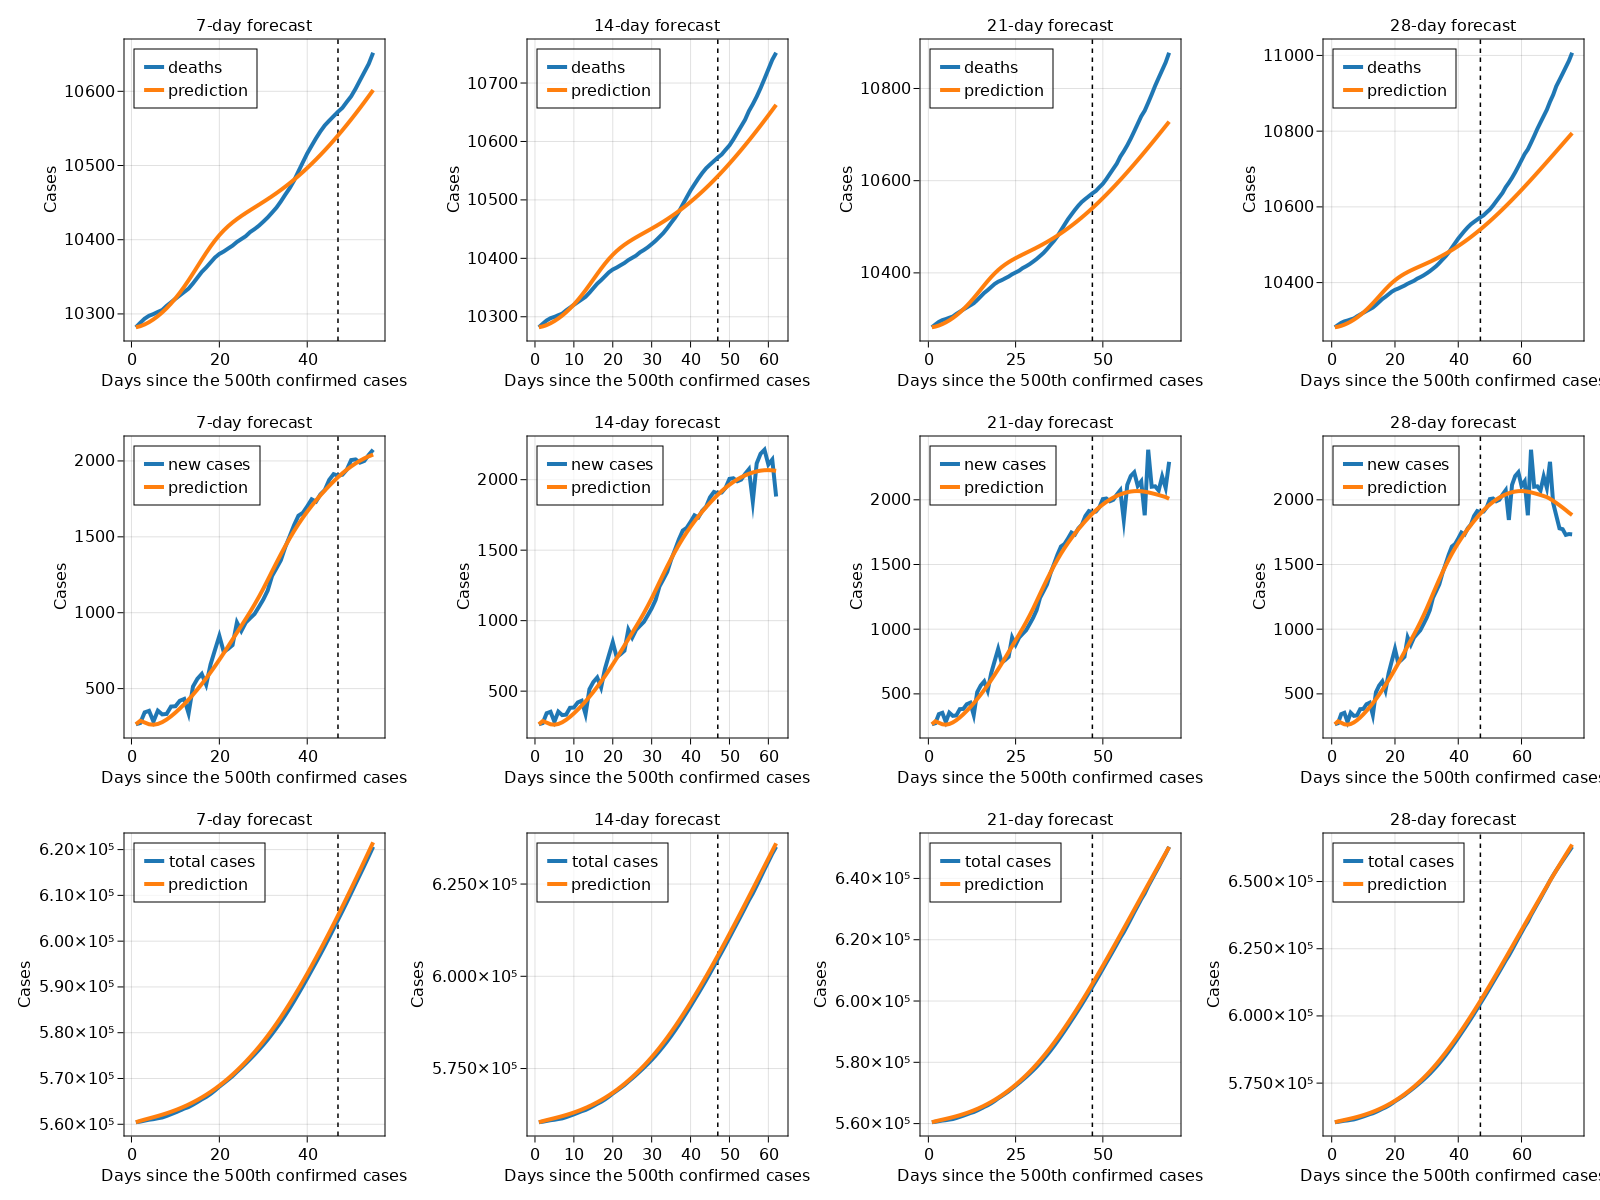
\includegraphics[scale=0.25]{fb1/maricopa_az/20211216131821.fbmobility1.maricopa_az.forecasts.png}
    \caption{Predictions made by the second version of the model that uses Facebook's Movement Range Maps dataset after having trained with data for Maricopa, Arizona. The black vertical dashed line marks the last day in the training period.}
    \label{fig:predictions-maricopa-fb1}
\end{figure}

\begin{figure}[!htb]
    \centering
    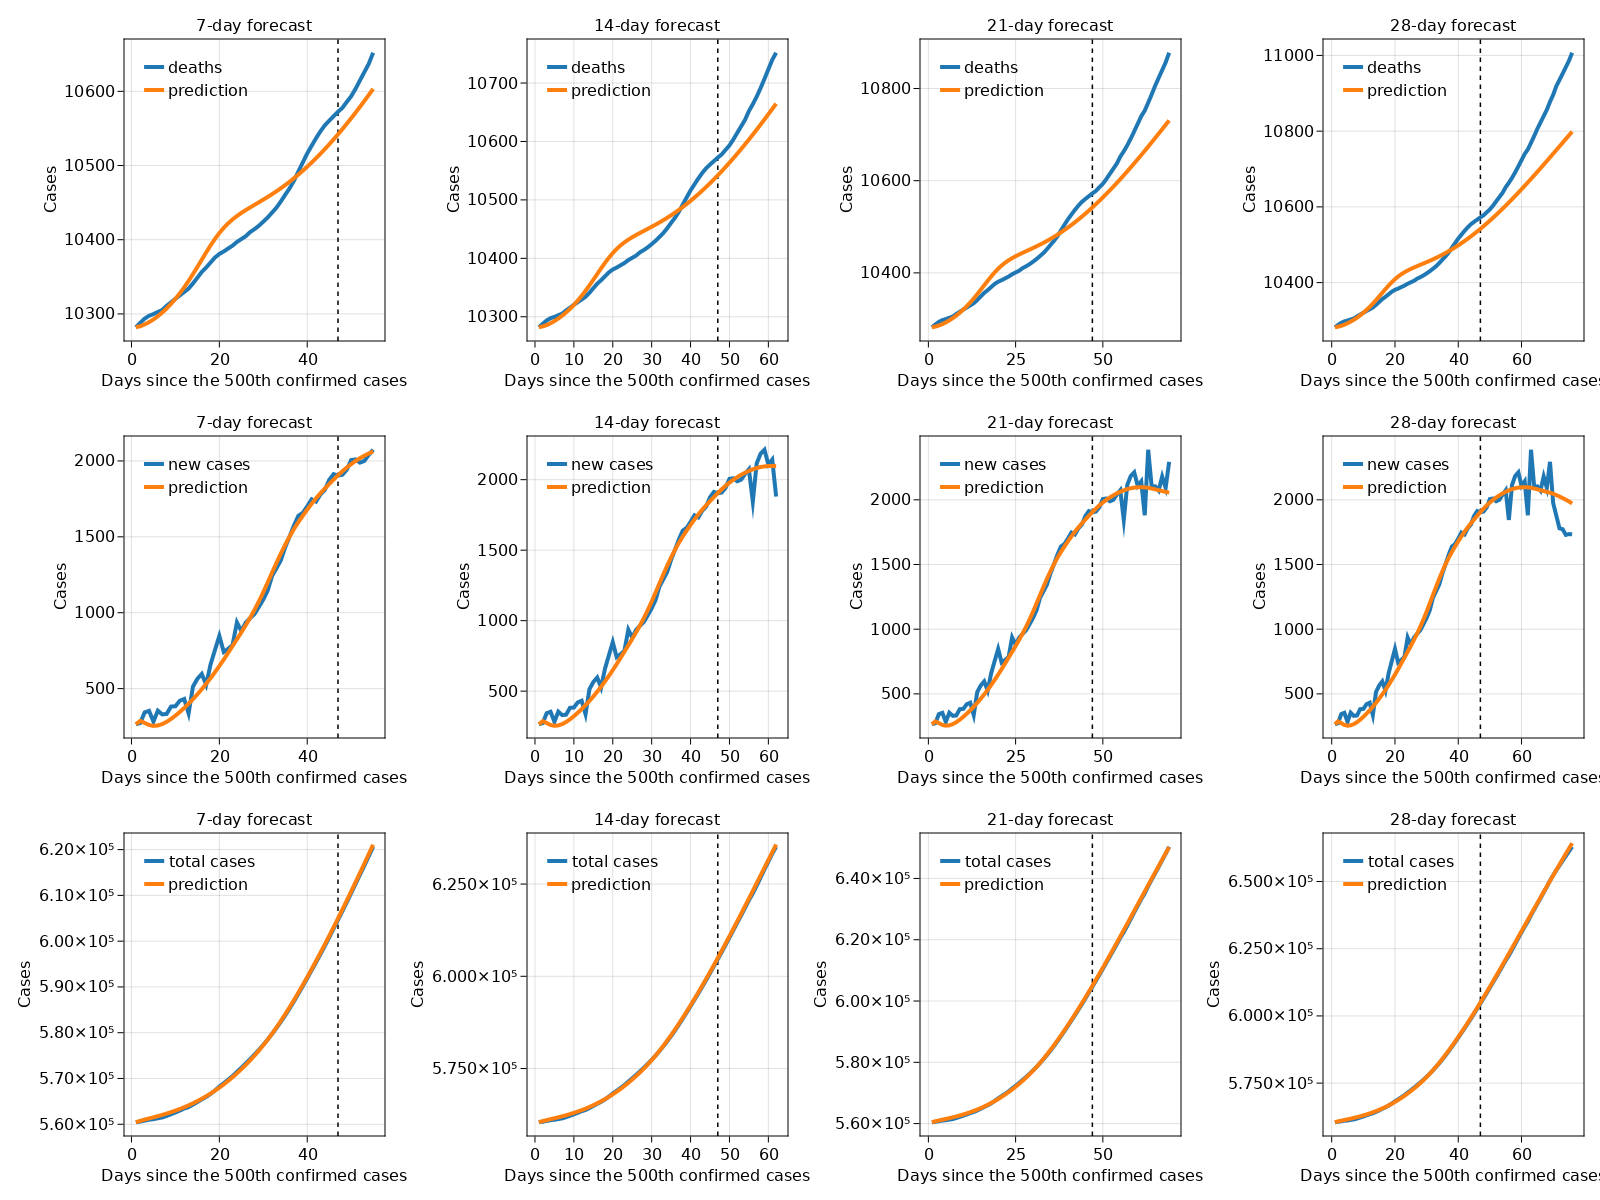
\includegraphics[scale=0.25]{fb2/maricopa_az/20211216193717.fbmobility2.maricopa_az.forecasts.png}
    \caption{Predictions made by the second version of the model that uses Facebook's Movement Range Maps dataset and Social Proximity to Cases Index after having trained with data for Maricopa, Arizona. The black vertical dashed line marks the last day in the training period.}
    \label{fig:predictions-maricopa-fb2}
\end{figure}

% BINH DUONG

\begin{figure}[!htb]
    \centering
    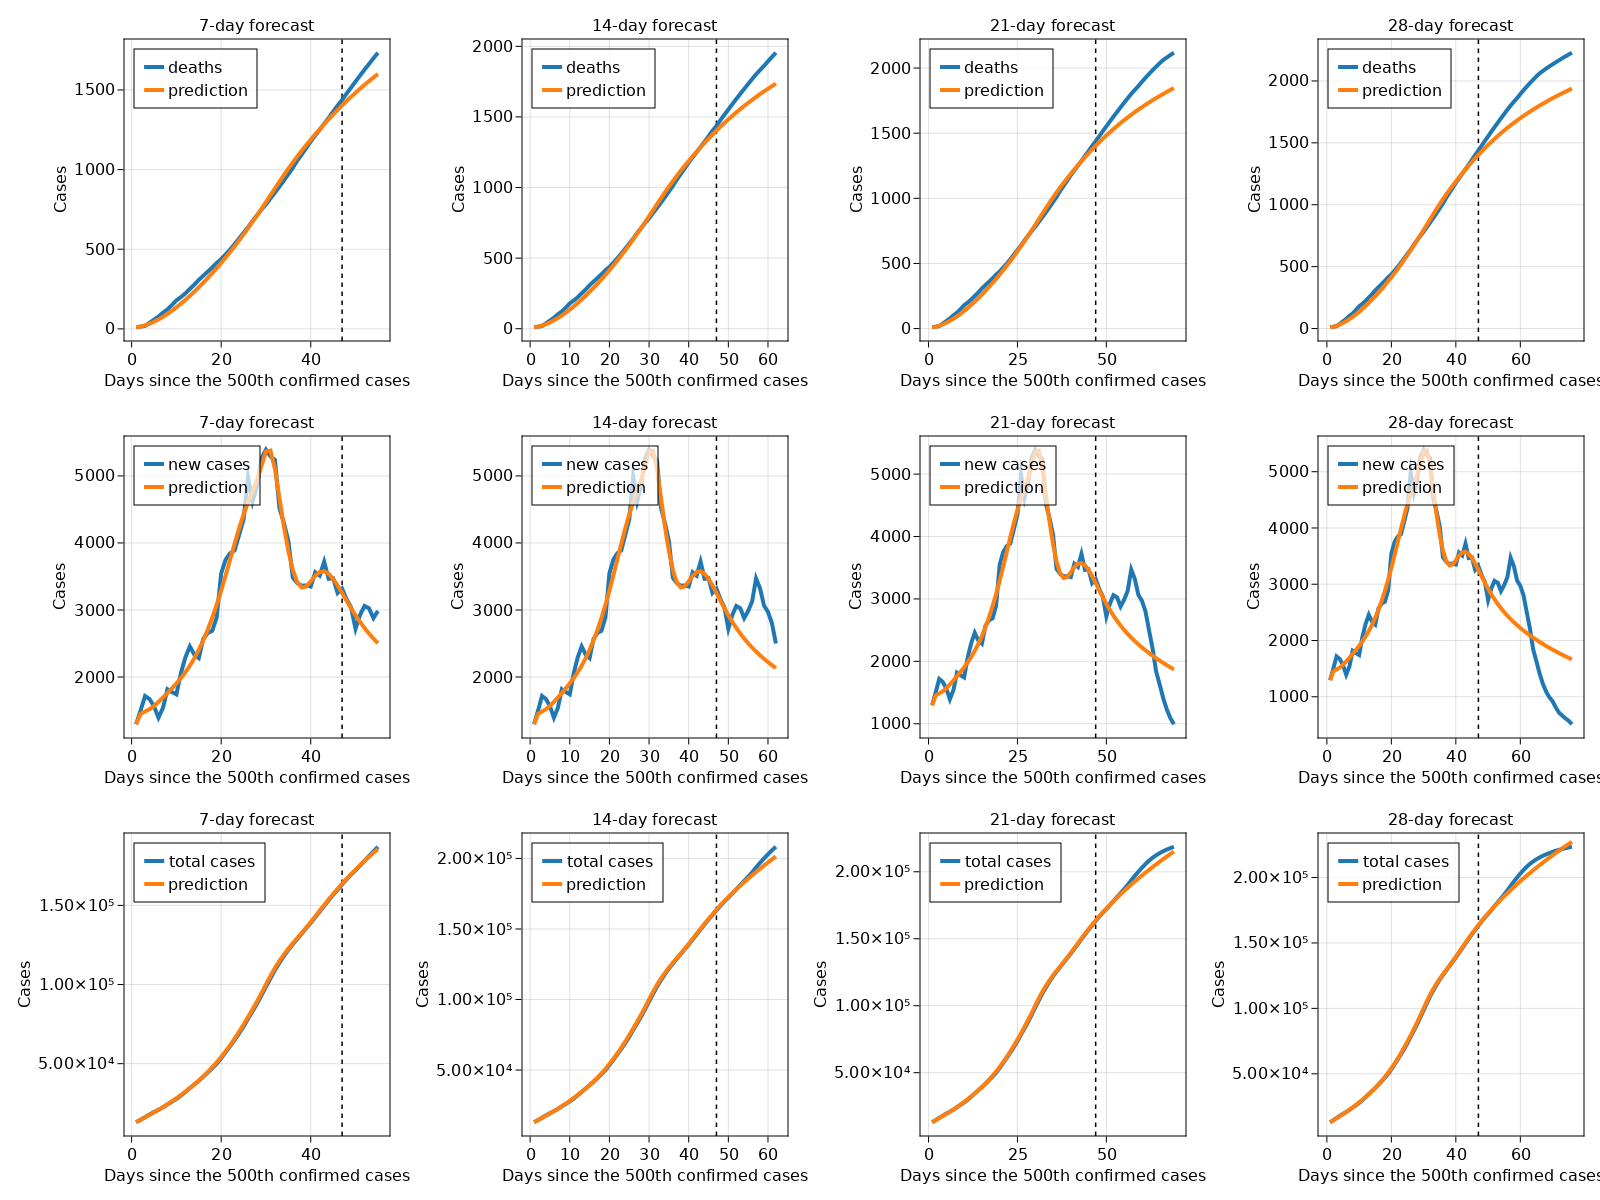
\includegraphics[scale=0.25]{baseline/binhduong/20211216111951.baseline.binhduong.forecasts.png}
    \caption{Predictions made by the baseline model after having trained with data for Binh Duong. The black vertical dashed line marks the last day in the training period.}
    \label{fig:predictions-binhduong-baseline}
\end{figure}

\begin{figure}[!htb]
    \centering
    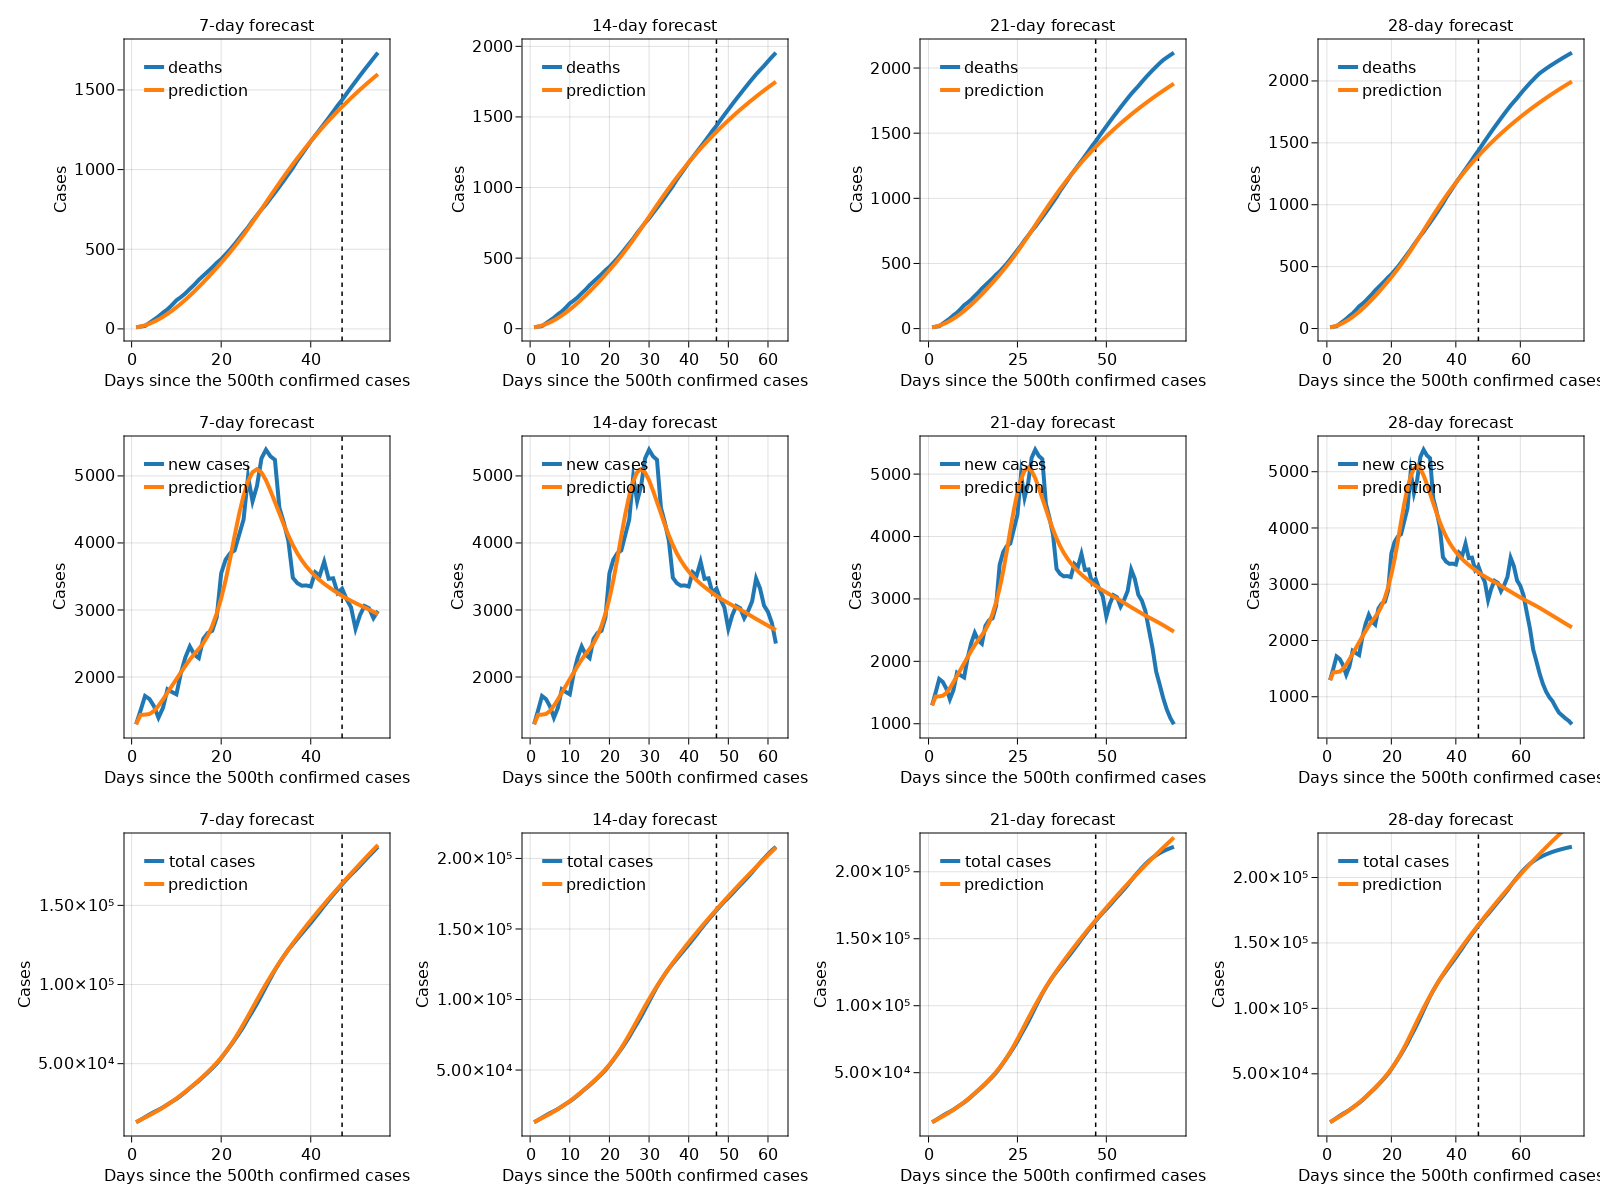
\includegraphics[scale=0.25]{fb1/binhduong/20211216173307.fbmobility1.binhduong.forecasts.png}
    \caption{Predictions made by the second version of the model that uses Facebook's Movement Range Maps dataset after having trained with data for Binh Duong. The black vertical dashed line marks the last day in the training period.}
    \label{fig:predictions-binhduong-fb1}
\end{figure}

\begin{figure}[!htb]
    \centering
    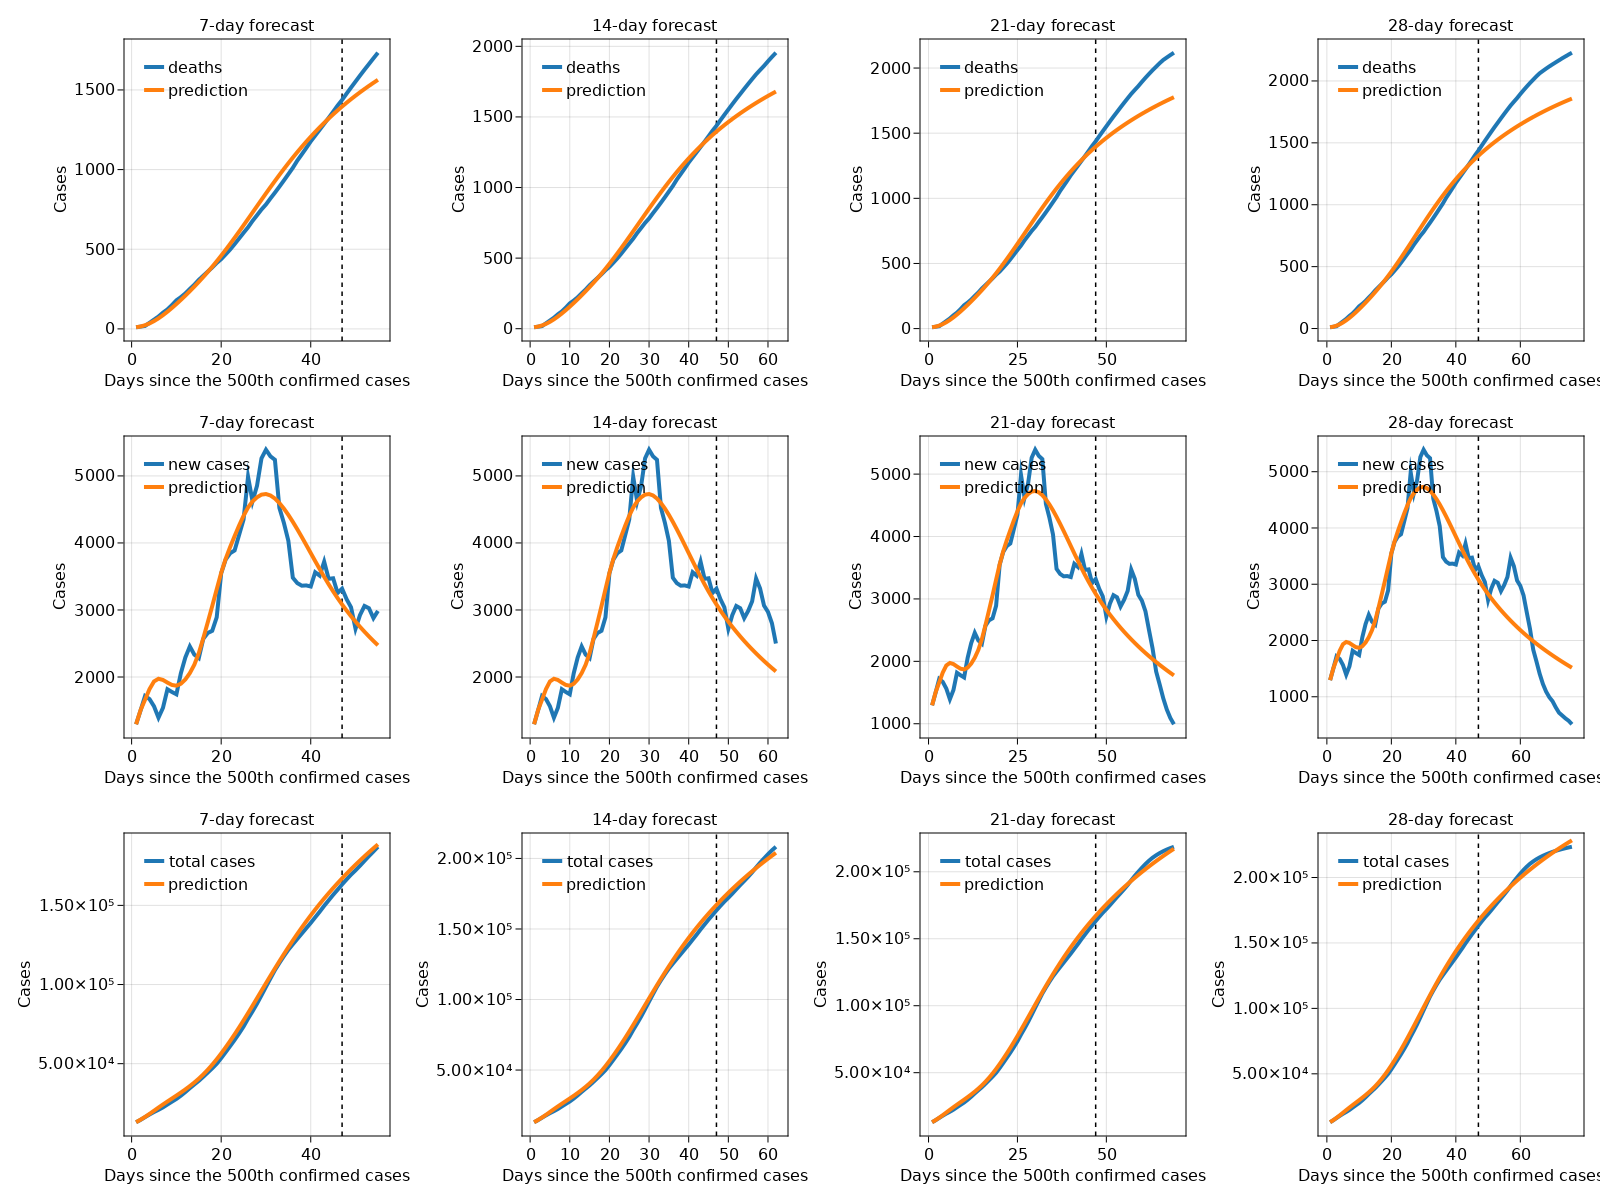
\includegraphics[scale=0.25]{fb2/binhduong/20211216172741.fbmobility2.binhduong.forecasts.png}
    \caption{Predictions made by the second version of the model that uses Facebook's Movement Range Maps dataset and Social Proximity to Cases Index after having trained with data for Binh duong. The black vertical dashed line marks the last day in the training period.}
    \label{fig:predictions-binhduong-fb2}
\end{figure}

% DONG NAI

\begin{figure}[!htb]
    \centering
    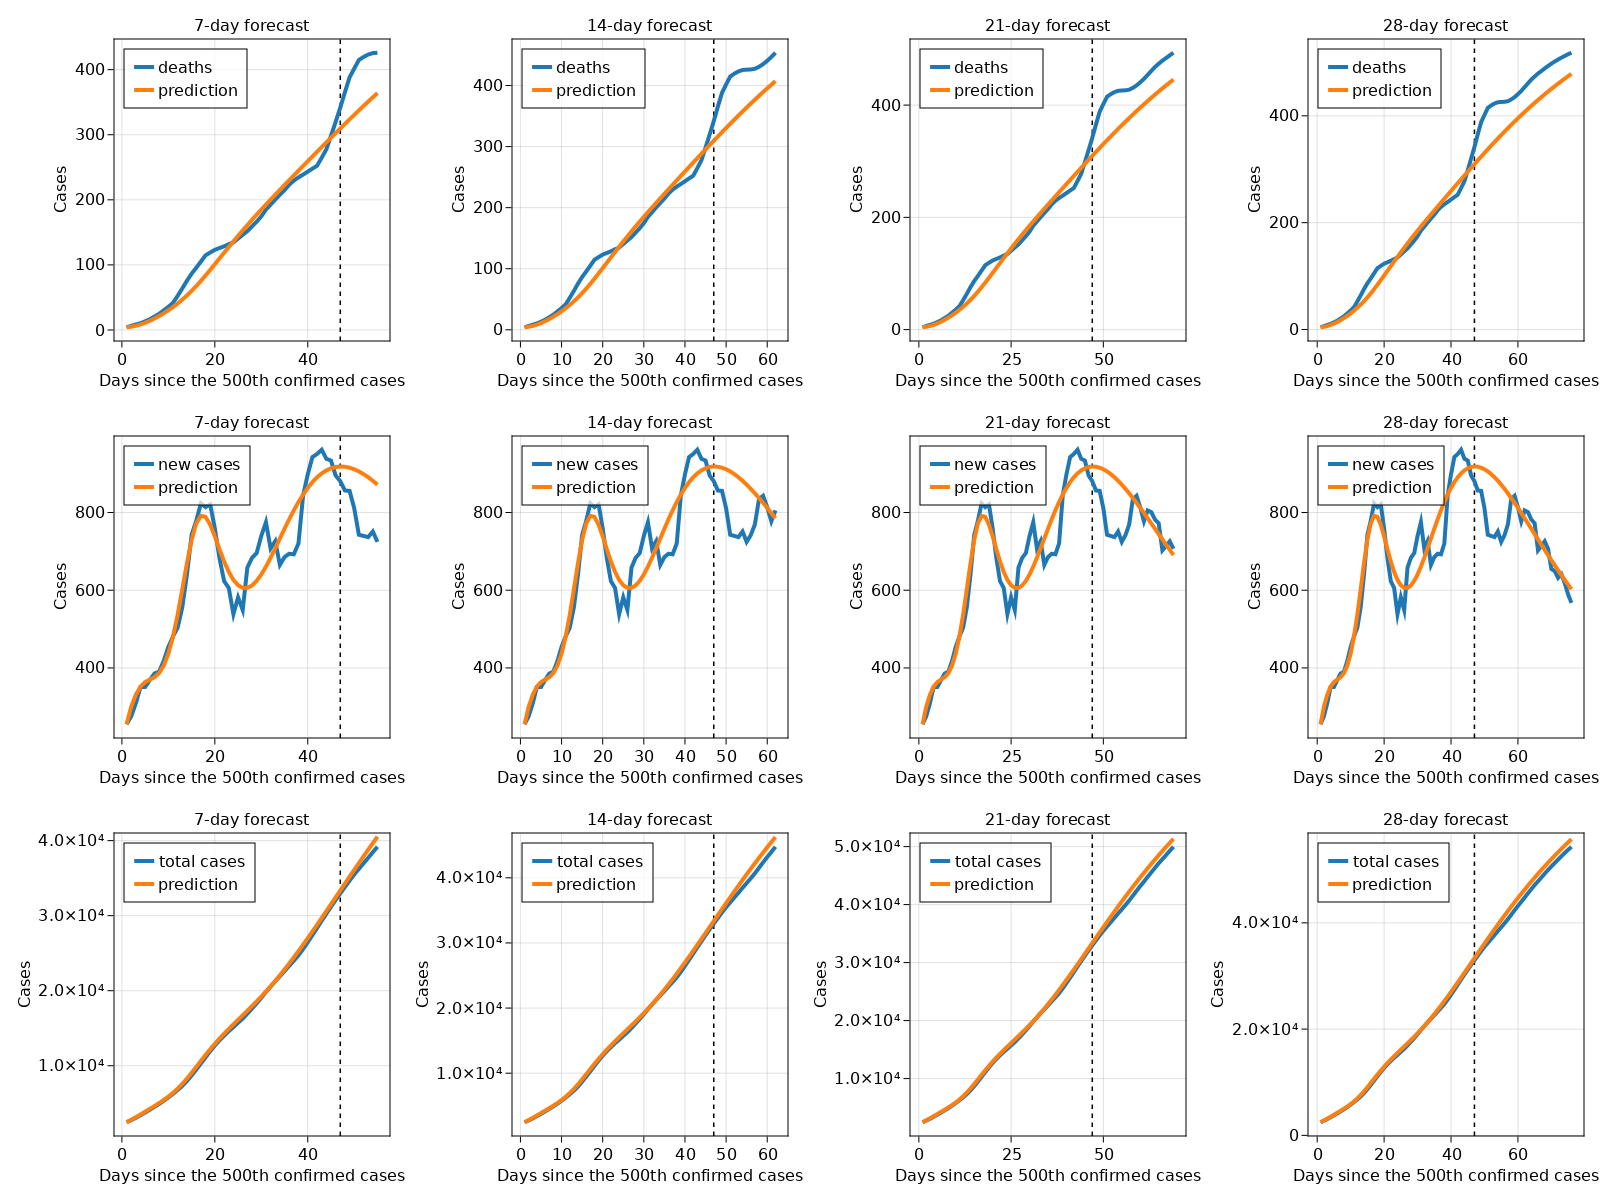
\includegraphics[scale=0.25]{baseline/dongnai/20211216211601.baseline.dongnai.forecasts.png}
    \caption{Predictions made by the baseline model after having trained with data for Dong Nai. The black vertical dashed line marks the last day in the training period.}
    \label{fig:predictions-dongnai-baseline}
\end{figure}

\begin{figure}[!htb]
    \centering
    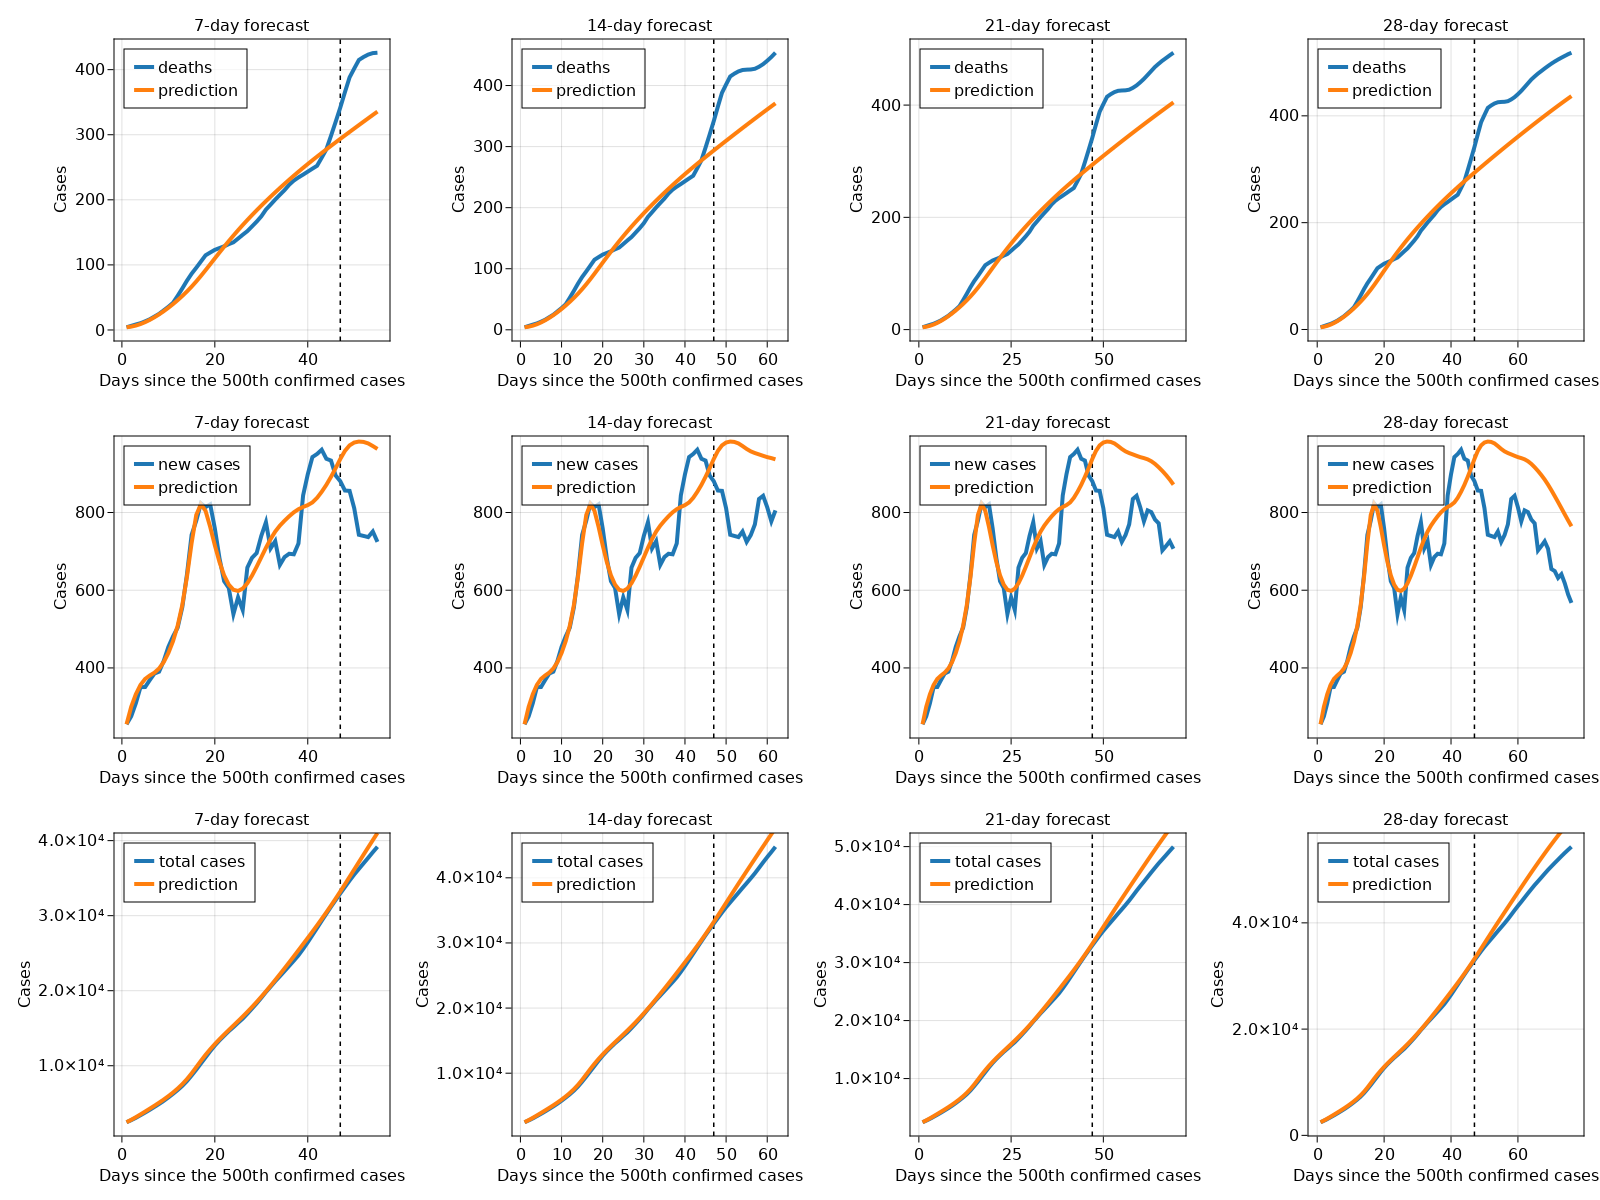
\includegraphics[scale=0.25]{fb1/dongnai/20211216131821.fbmobility1.dongnai.forecasts.png}
    \caption{Predictions made by the second version of the model that uses Facebook's Movement Range Maps dataset after having trained with data for Dong Nai. The black vertical dashed line marks the last day in the training period.}
    \label{fig:predictions-dongnai-fb1}
\end{figure}

\begin{figure}[!htb]
    \centering
    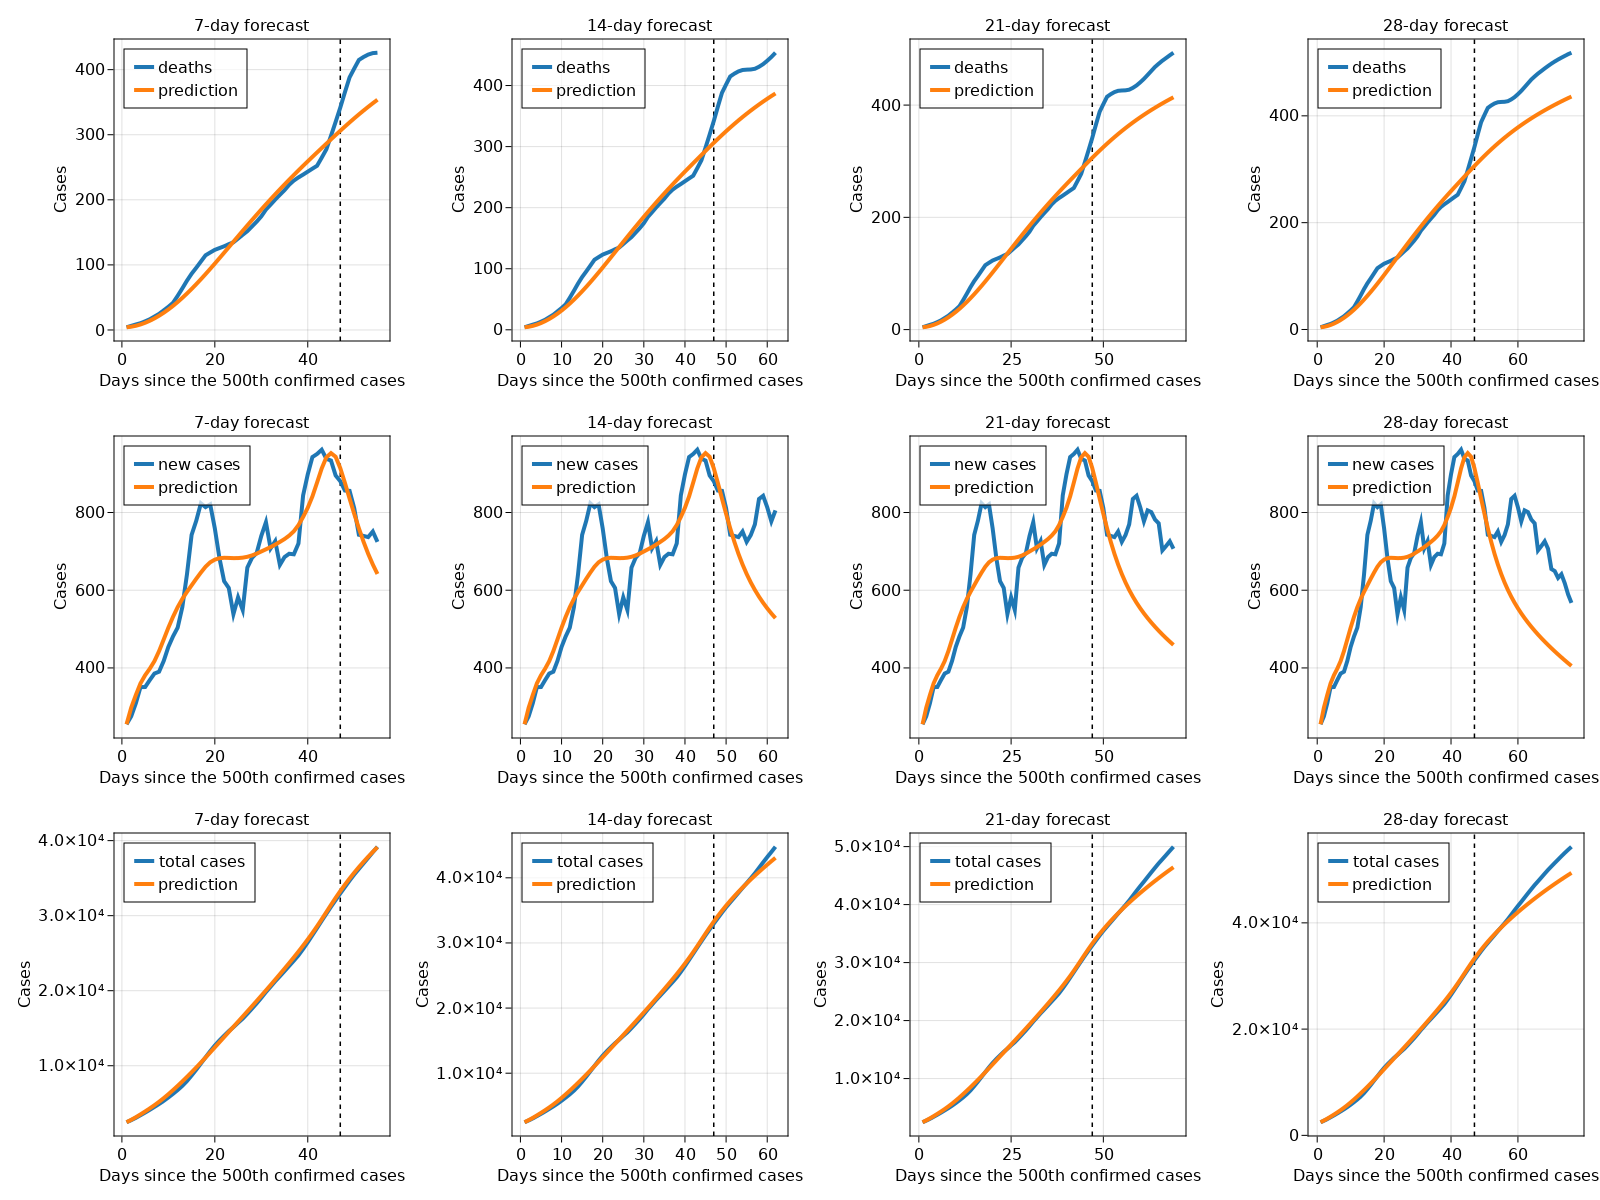
\includegraphics[scale=0.25]{fb2/dongnai/20211217220549.fbmobility2.dongnai.forecasts.png}
    \caption{Predictions made by the second version of the model that uses Facebook's Movement Range Maps dataset and Social Proximity to Cases Index after having trained with data for Dong Nai. The black vertical dashed line marks the last day in the training period.}
    \label{fig:predictions-dongnai-fb2}
\end{figure}

% HO CHI MINH CITY

\begin{figure}[!htb]
    \centering
    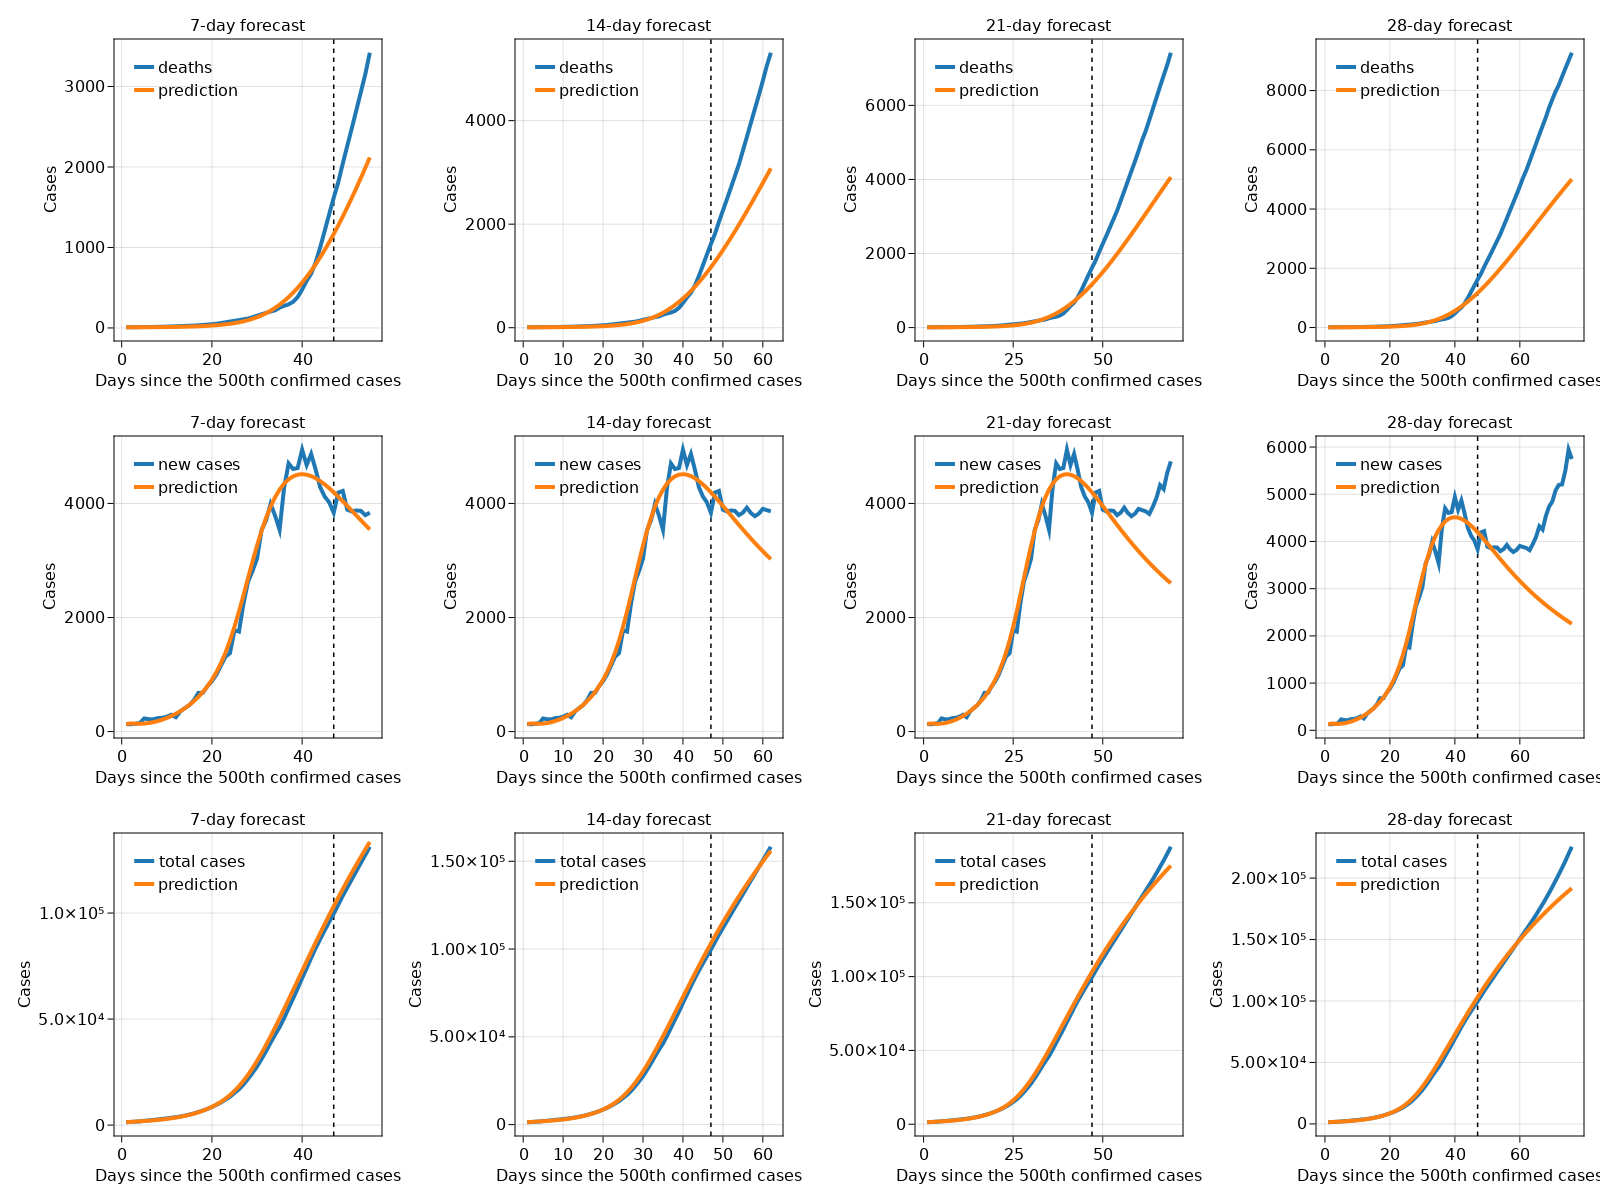
\includegraphics[scale=0.25]{baseline/hcm/20211216154445.baseline.hcm.forecasts.png}
    \caption{Predictions made by the baseline model after having trained with data for Ho Chi Minh city. The black vertical dashed line marks the last day in the training period.}
    \label{fig:predictions-hcm-baseline}
\end{figure}

\begin{figure}[!htb]
    \centering
    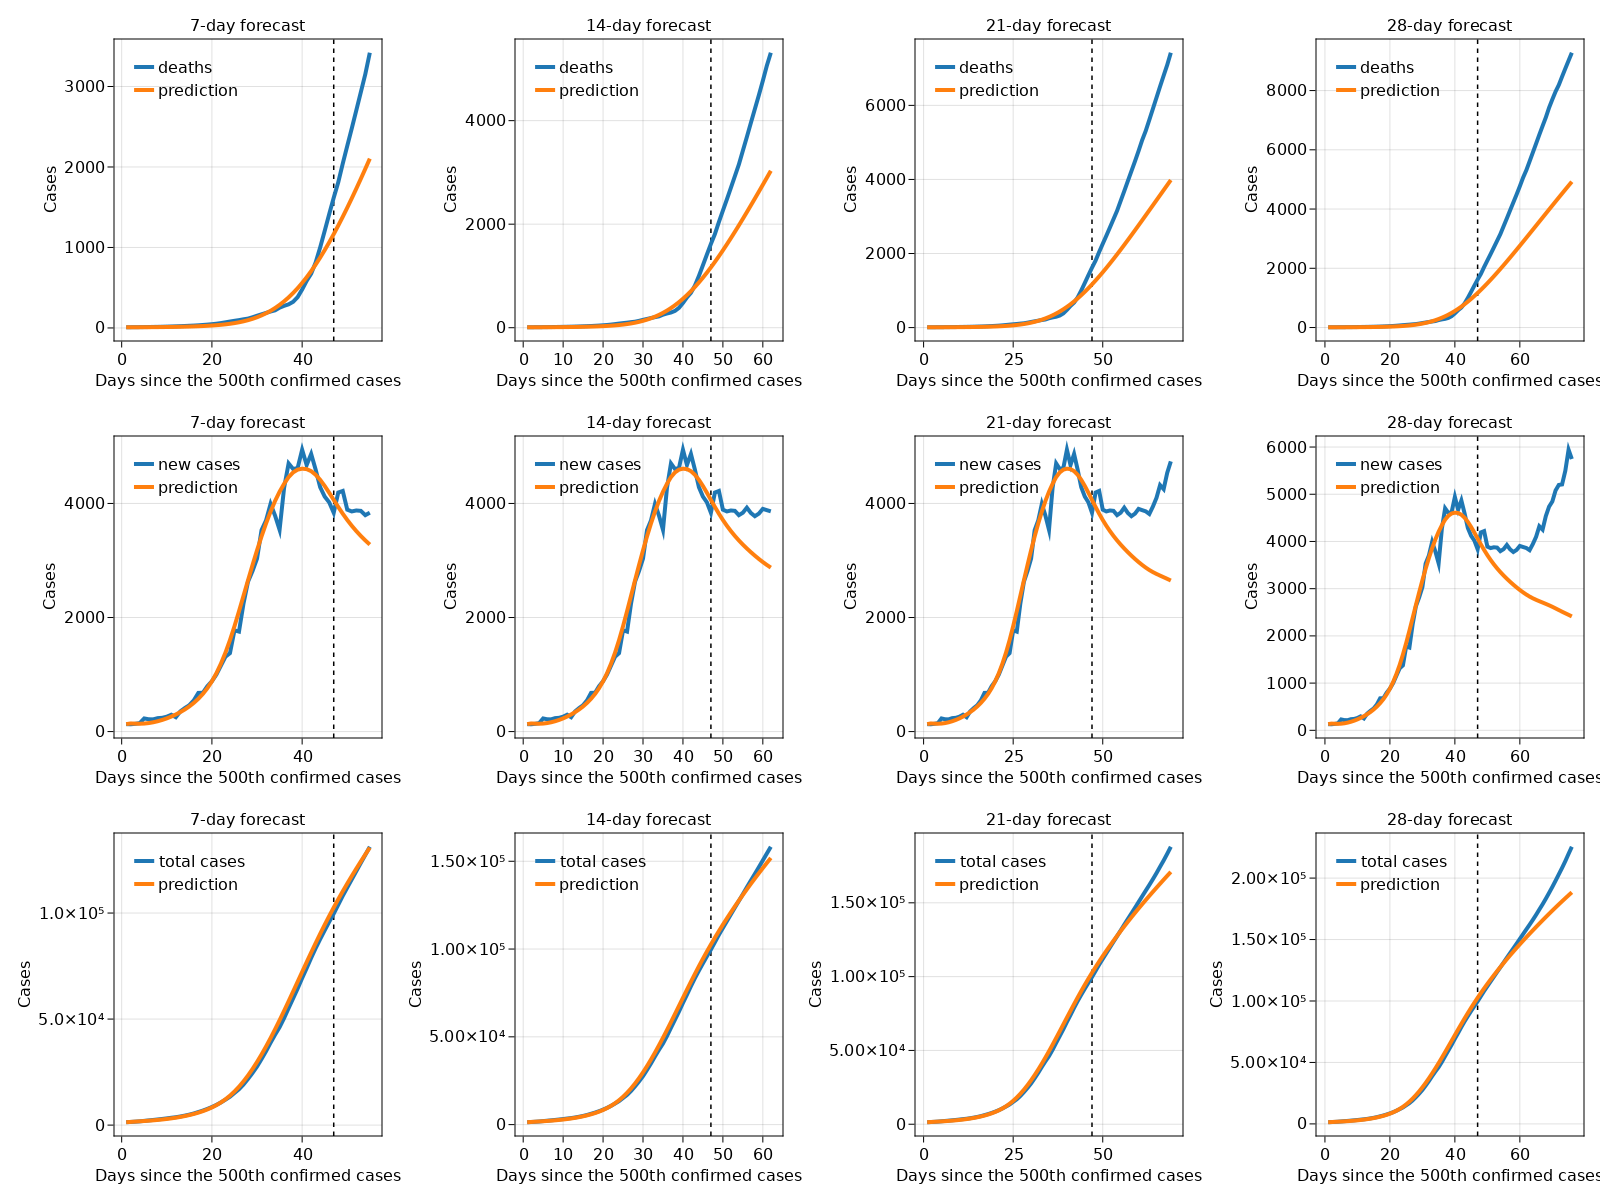
\includegraphics[scale=0.25]{fb1/hcm/20211216231719.fbmobility1.hcm.forecasts.png}
    \caption{Predictions made by the second version of the model that uses Facebook's Movement Range Maps dataset after having trained with data for Ho Chi Minh city. The black vertical dashed line marks the last day in the training period.}
    \label{fig:predictions-hcm-fb1}
\end{figure}

\begin{figure}[!htb]
    \centering
    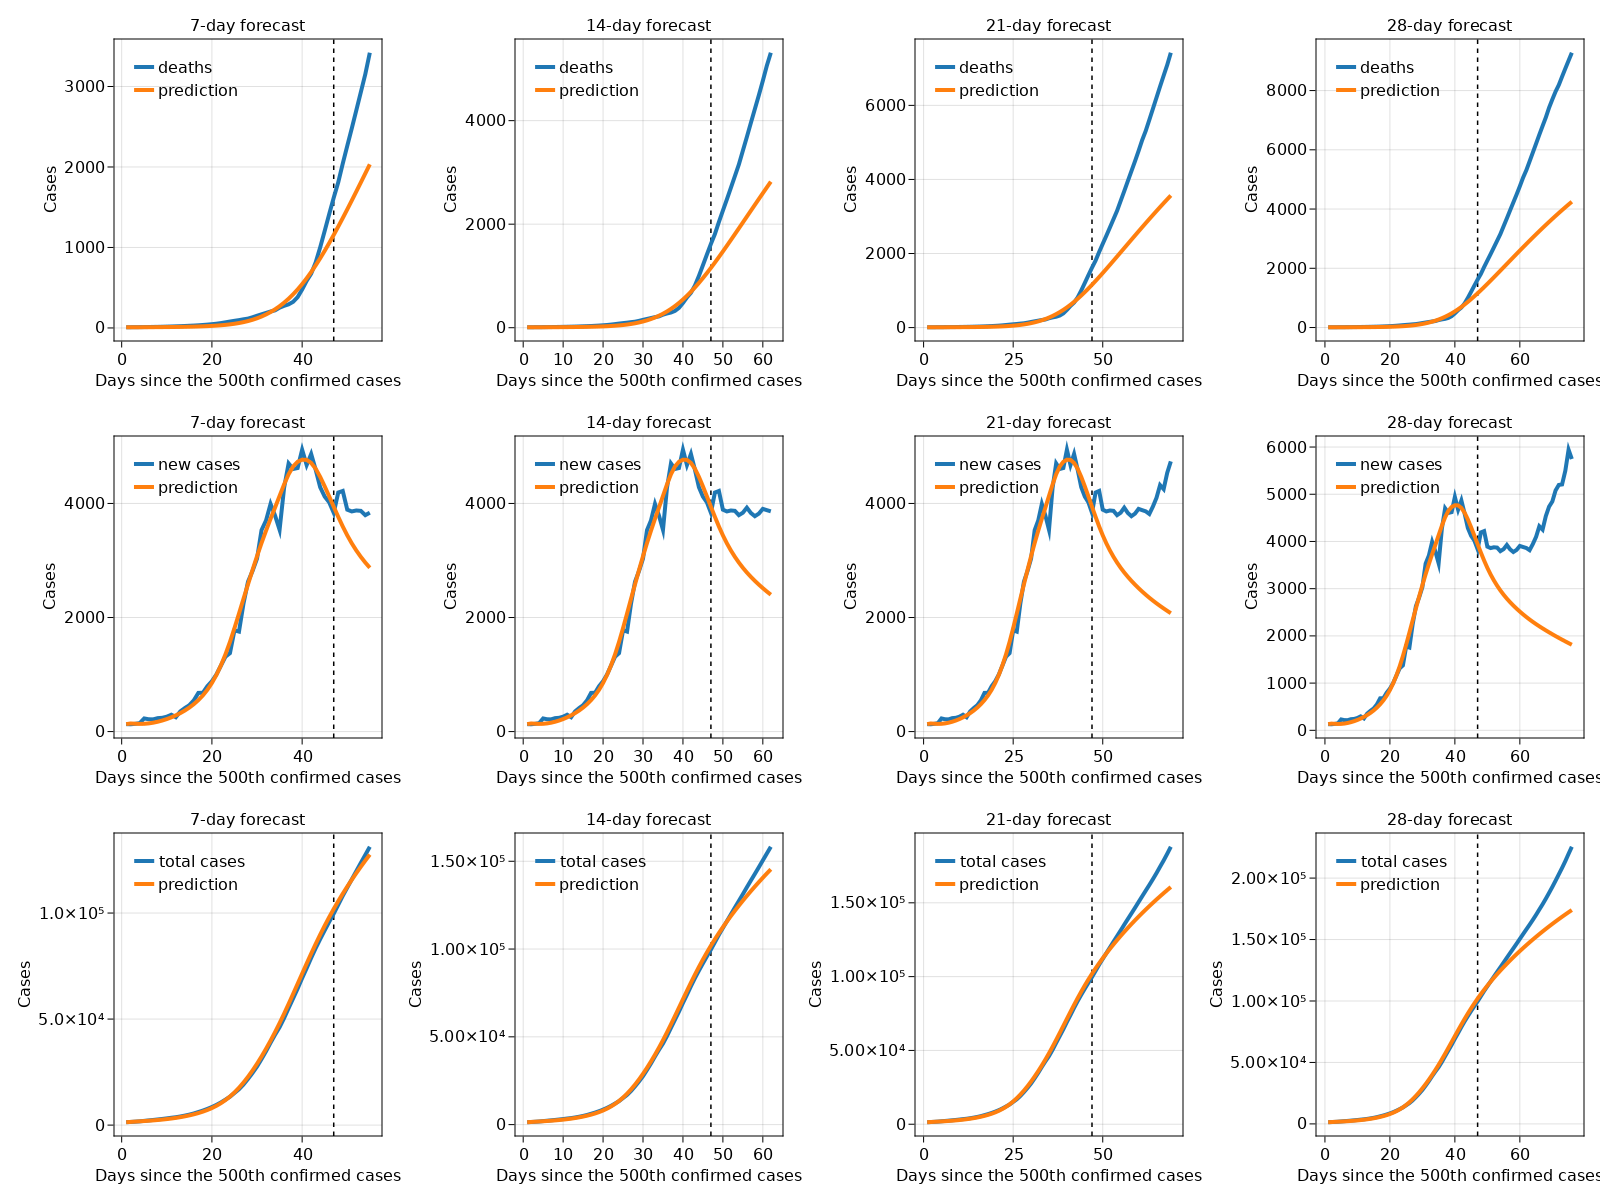
\includegraphics[scale=0.25]{fb2/hcm/20211216183635.fbmobility2.hcm.forecasts.png}
    \caption{Predictions made by the second version of the model that uses Facebook's Movement Range Maps dataset and Social Proximity to Cases Index after having trained with data for Ho Chi Minh city. The black vertical dashed line marks the last day in the training period.}
    \label{fig:predictions-hcm-fb2}
\end{figure}

% LONG AN

\begin{figure}[!htb]
    \centering
    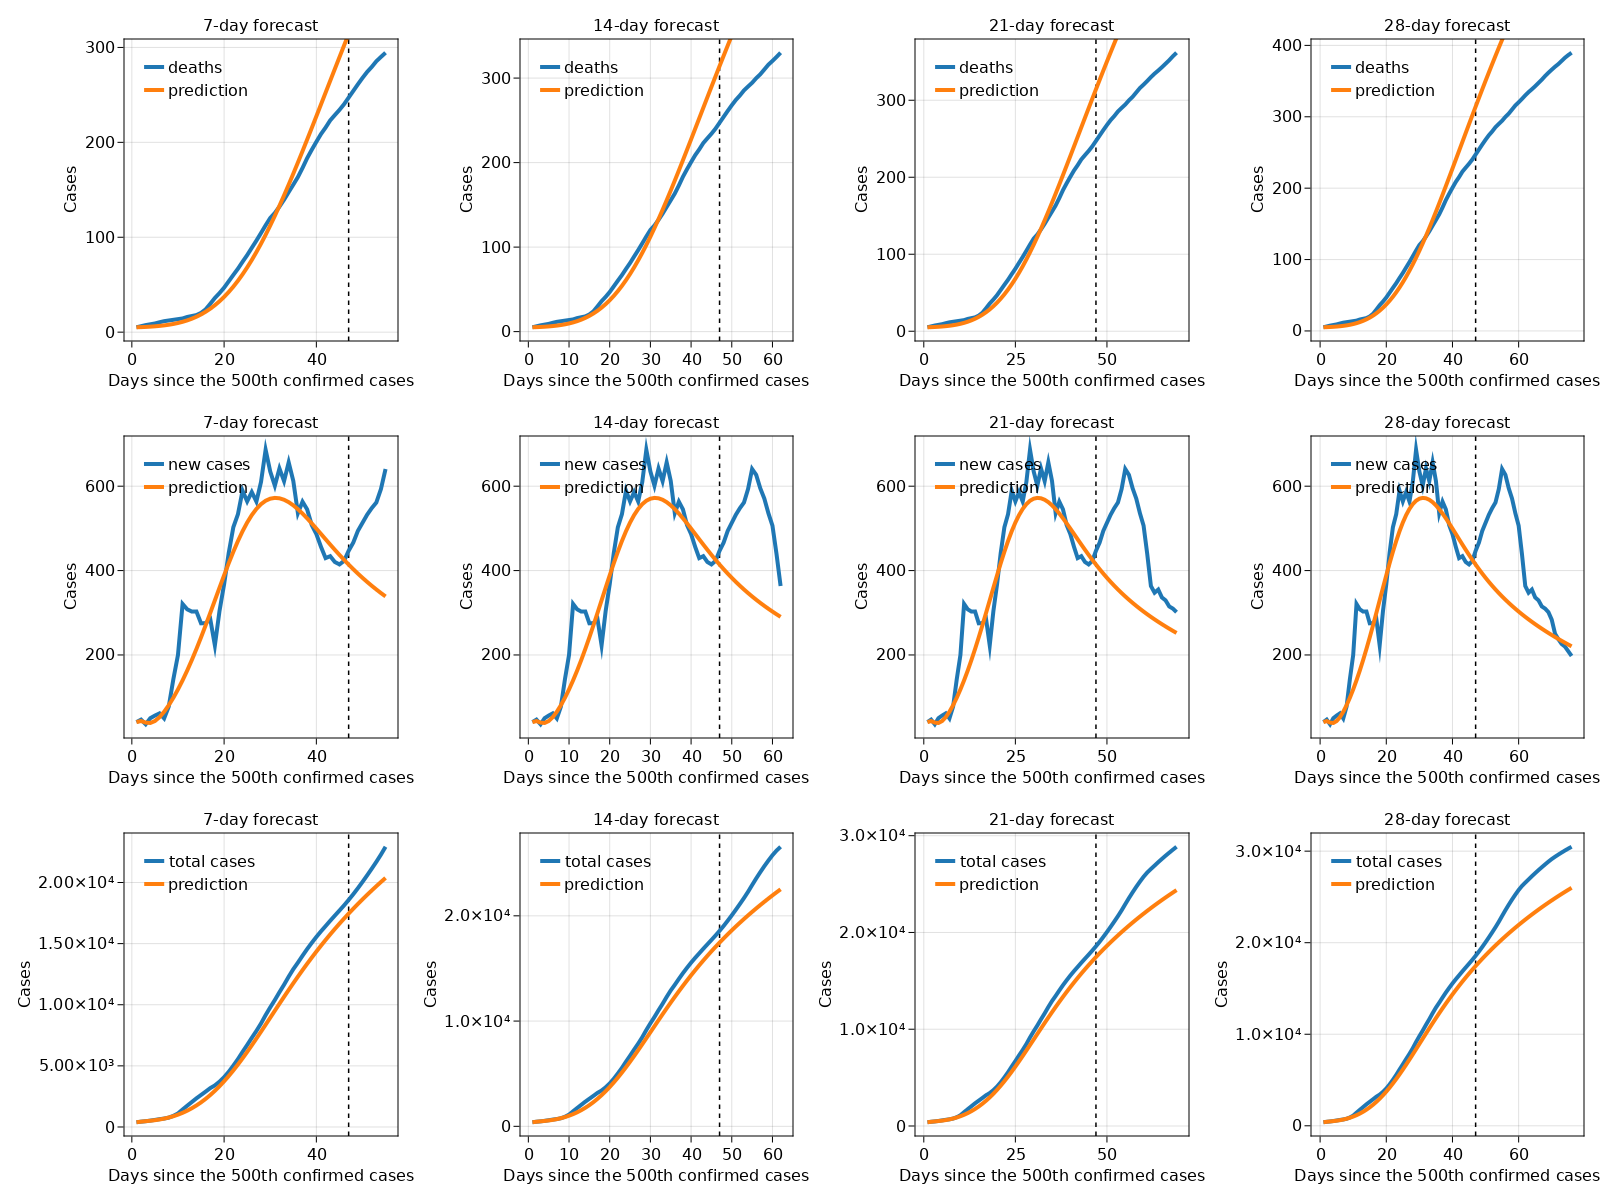
\includegraphics[scale=0.25]{baseline/longan/20211216111951.baseline.longan.forecasts.png}
    \caption{Predictions made by the baseline model after having trained with data for Long An. The black vertical dashed line marks the last day in the training period.}
    \label{fig:predictions-longan-baseline}
\end{figure}

\begin{figure}[!htb]
    \centering
    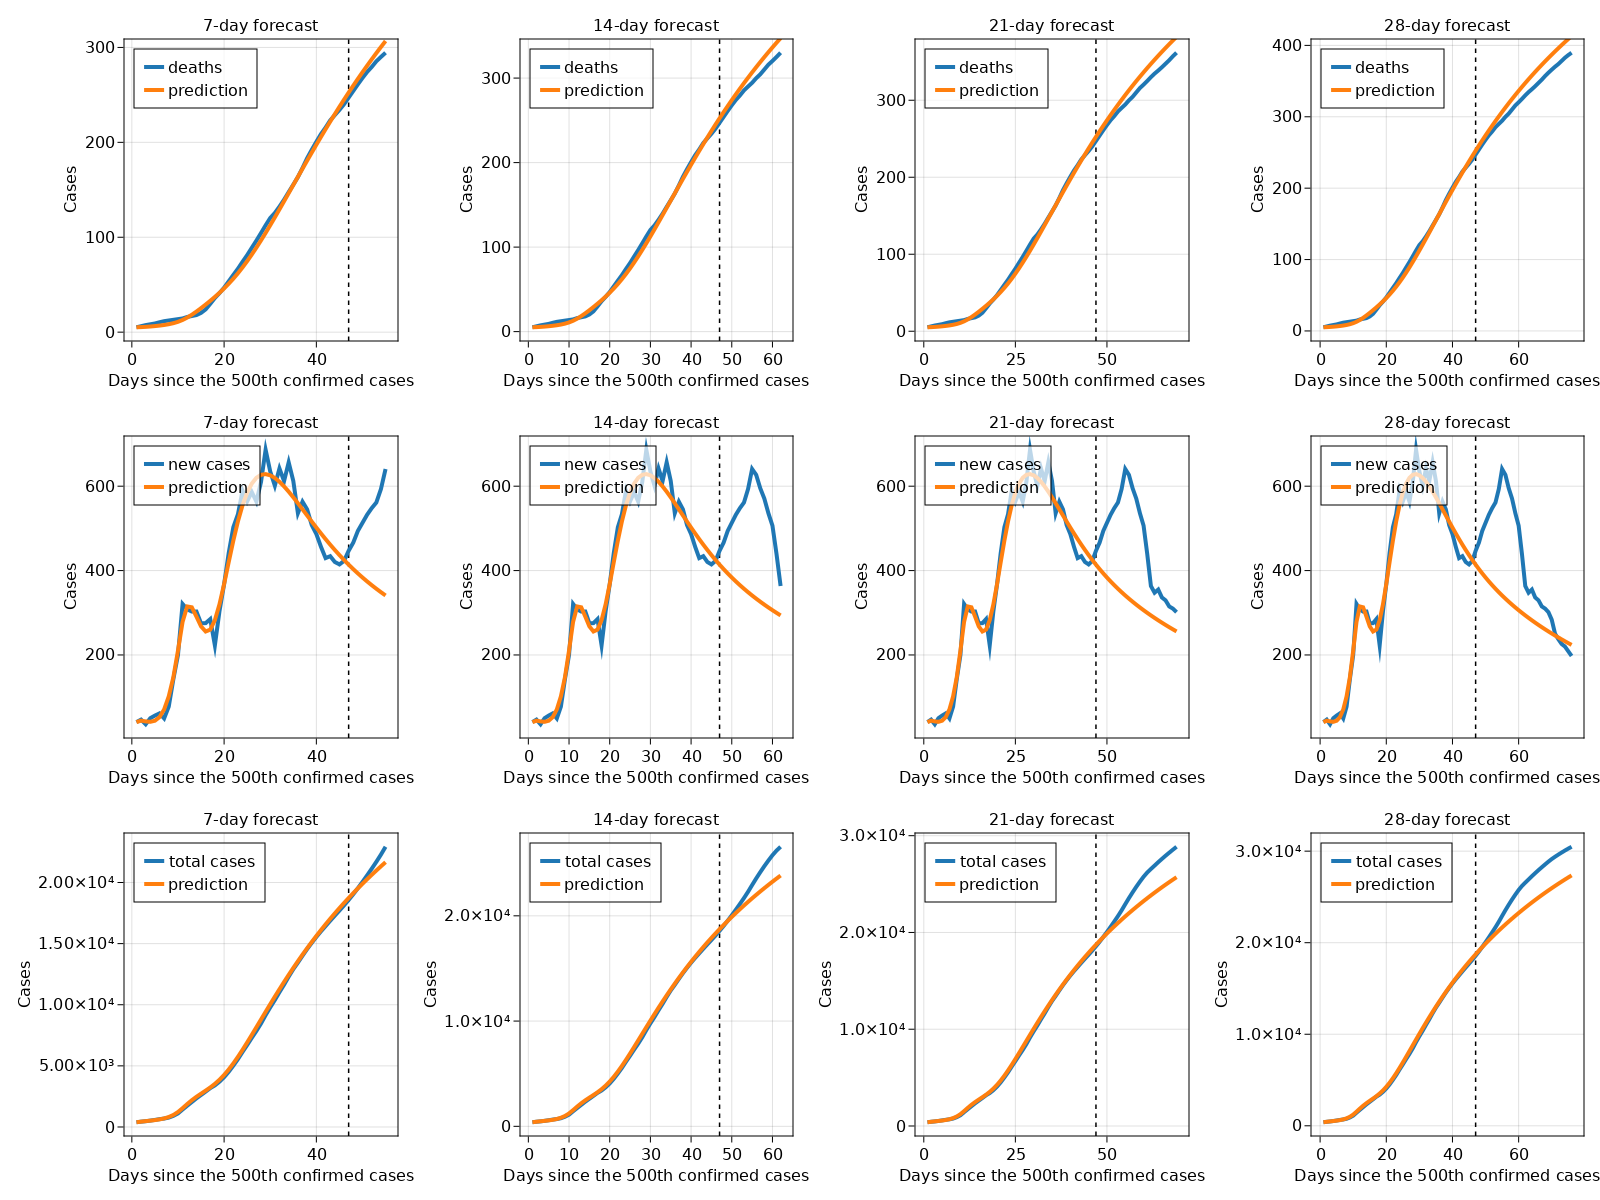
\includegraphics[scale=0.25]{fb1/longan/20211216131821.fbmobility1.longan.forecasts.png}
    \caption{Predictions made by the second version of the model that uses Facebook's Movement Range Maps dataset after having trained with data for Long An. The black vertical dashed line marks the last day in the training period.}
    \label{fig:predictions-longan-fb1}
\end{figure}

\begin{figure}[!htb]
    \centering
    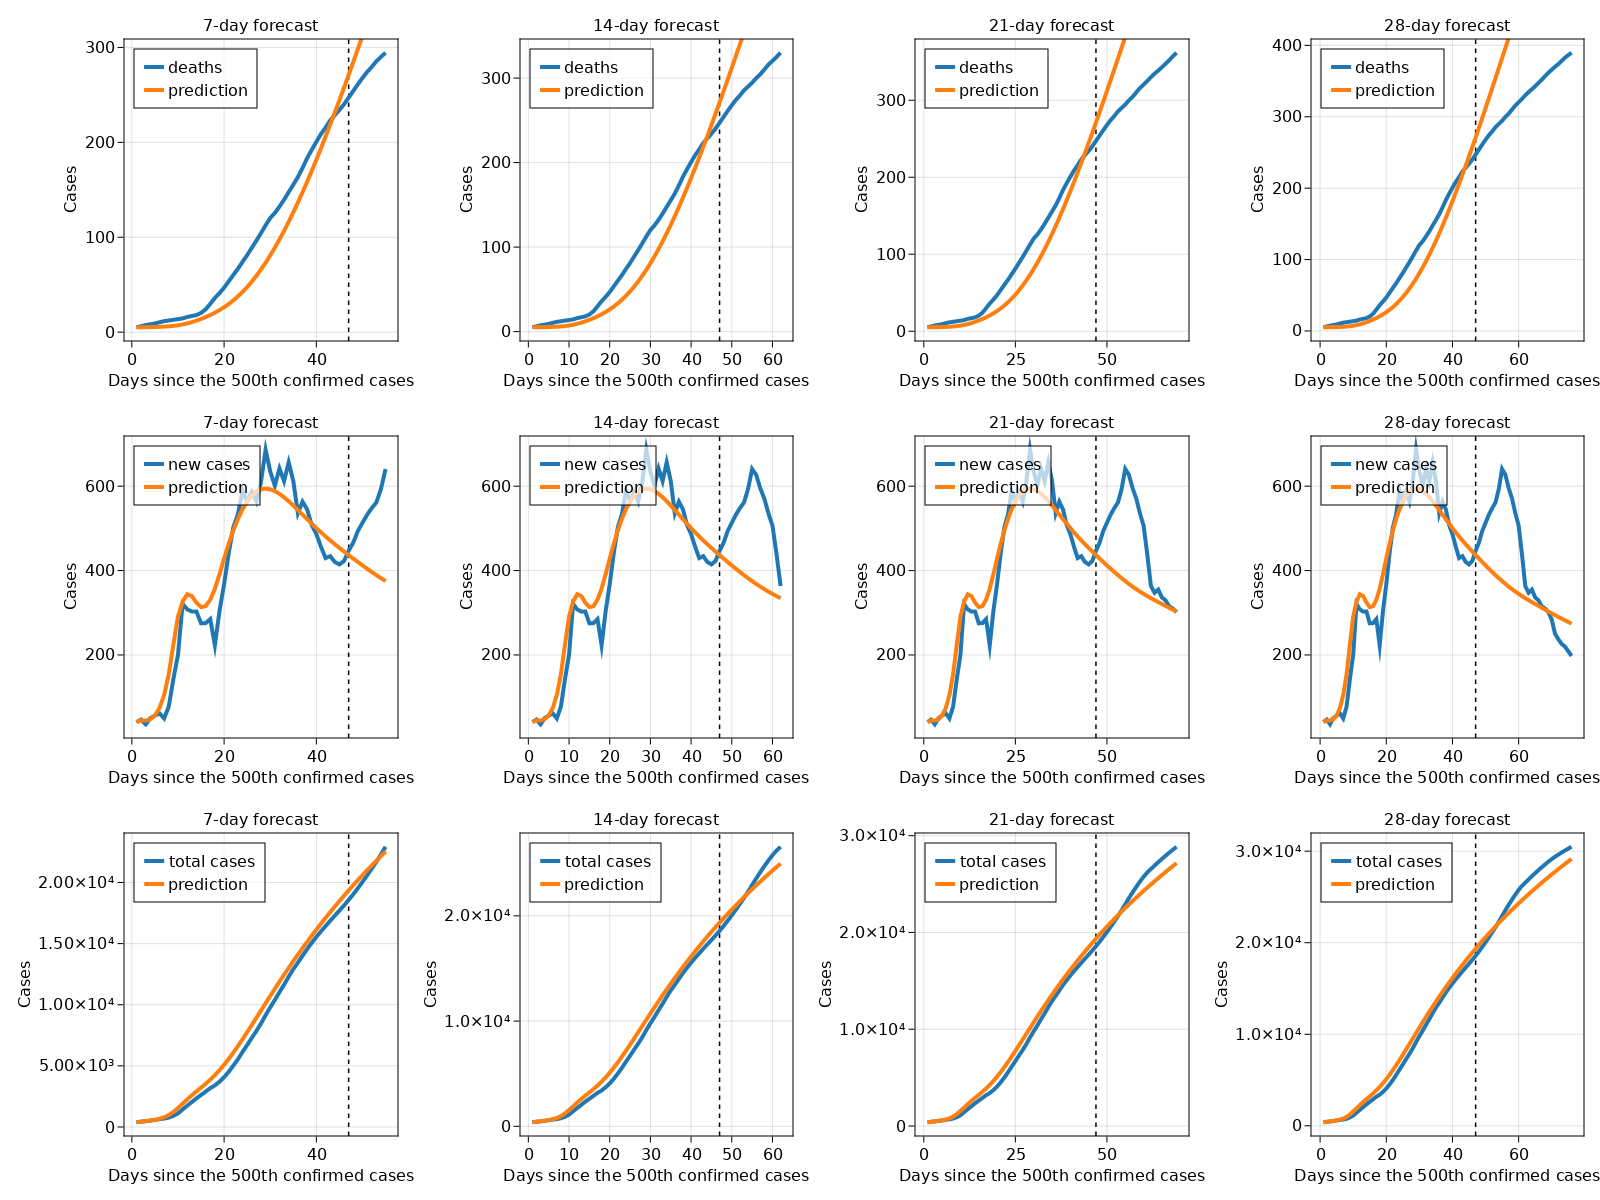
\includegraphics[scale=0.25]{fb2/longan/20211216193717.fbmobility2.longan.forecasts.png}
    \caption{Predictions made by the second version of the model that uses Facebook's Movement Range Maps dataset and Social Proximity to Cases Index after having trained with data for Long An. The black vertical dashed line marks the last day in the training period.}
    \label{fig:predictions-longan-fb2}
\end{figure}

% ======== LITERATURE REVIEW ========
\appendix

\chapter{Model predictions}

% VIETNAM

\begin{figure}[!htb]
    \centering
    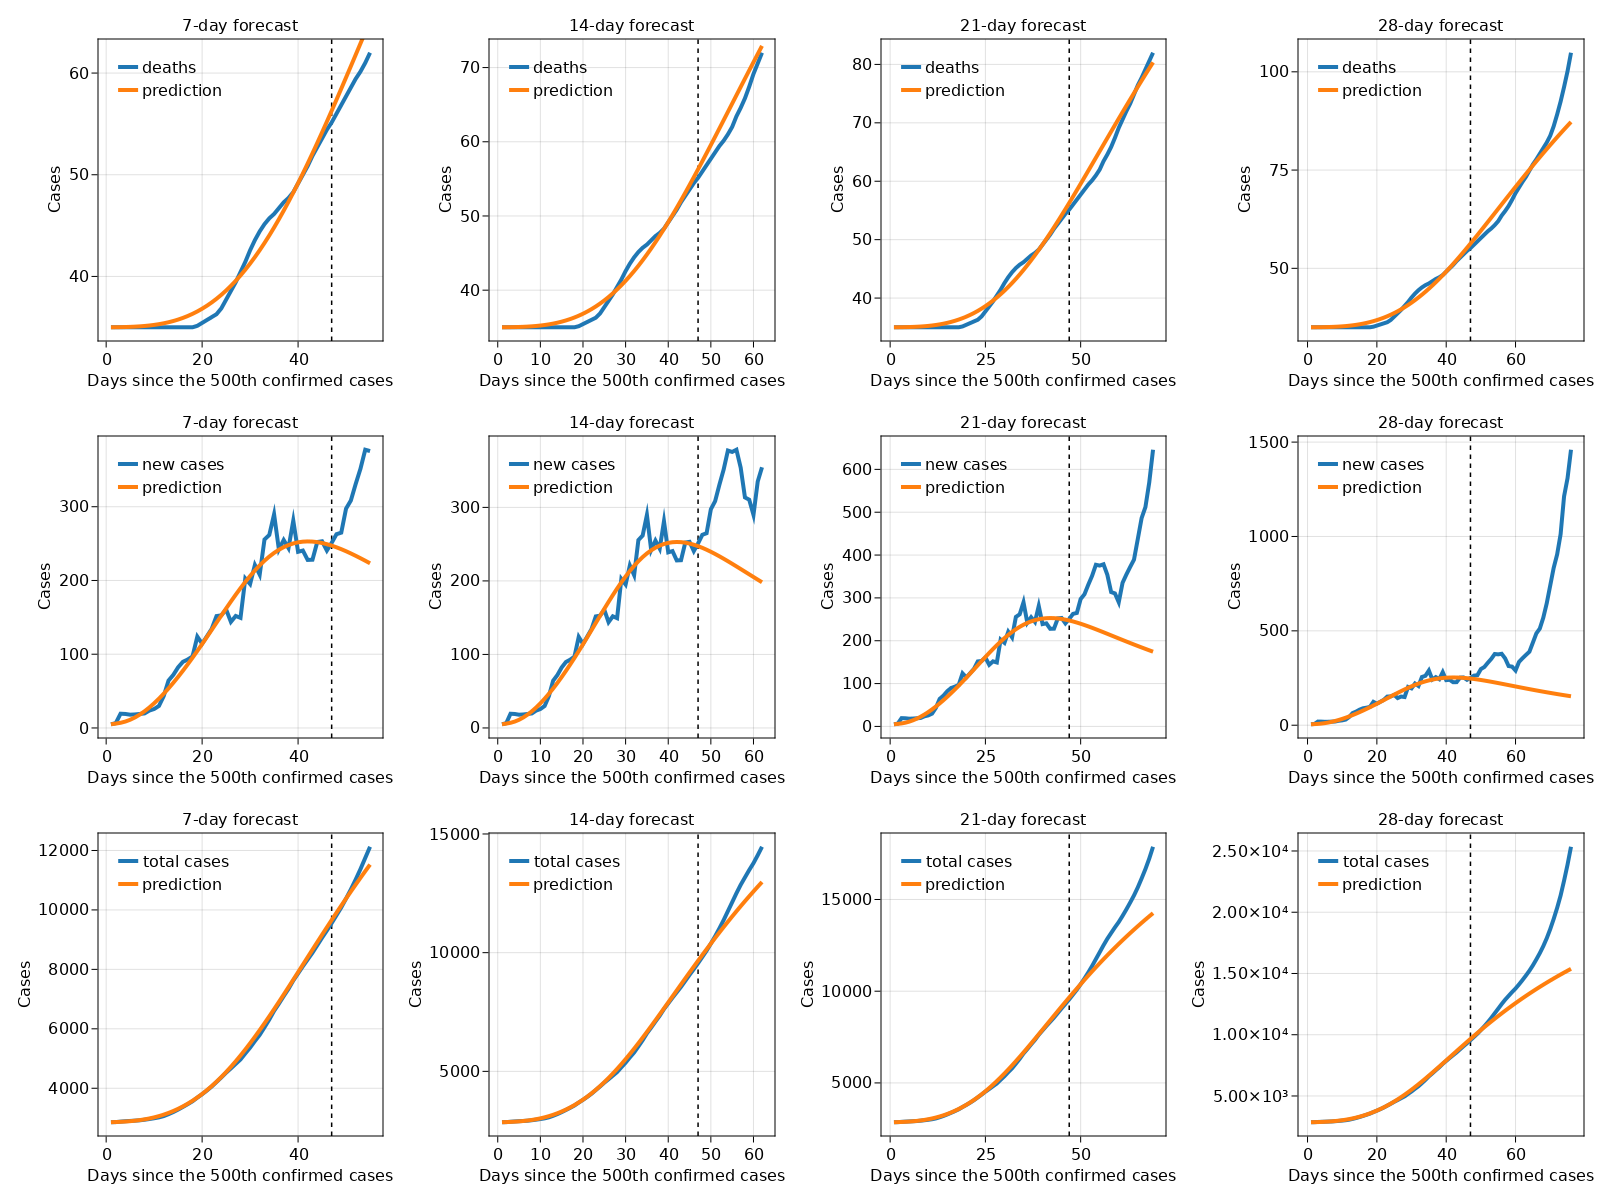
\includegraphics[scale=0.25]{baseline/vietnam/20211216111951.baseline.vietnam.forecasts.png}
    \caption{Predictions made by the baseline model after having trained with data for Vietnam. The black vertical dashed line marks the last day in the training period.}
    \label{fig:predictions-vietnam-baseline}
\end{figure}

\begin{figure}[!htb]
    \centering
    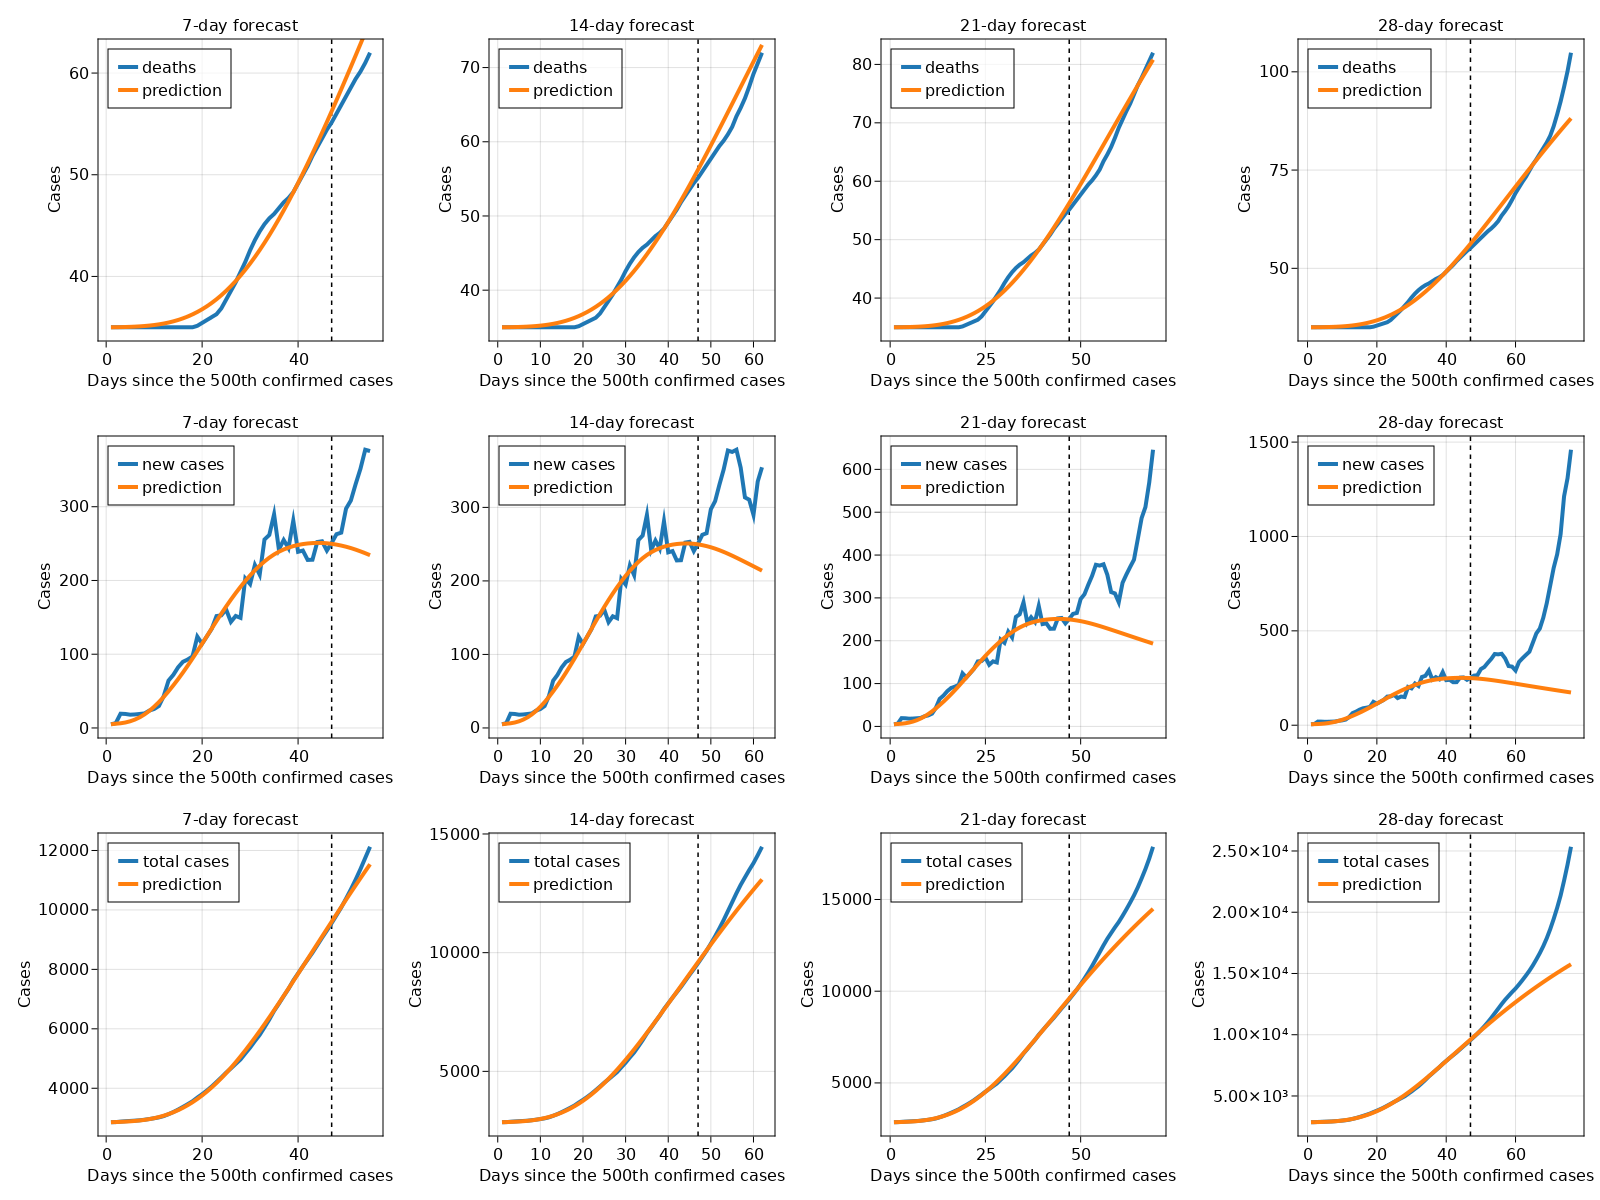
\includegraphics[scale=0.25]{fb1/vietnam/20211216231719.fbmobility1.vietnam.forecasts.png}
    \caption{Predictions made by the second version of the model that uses Facebook's Movement Range Maps dataset after having trained with data for Vietnam. The black vertical dashed line marks the last day in the training period.}
    \label{fig:predictions-vietnam-fb1}
\end{figure}

% US

\begin{figure}[!htb]
    \centering
    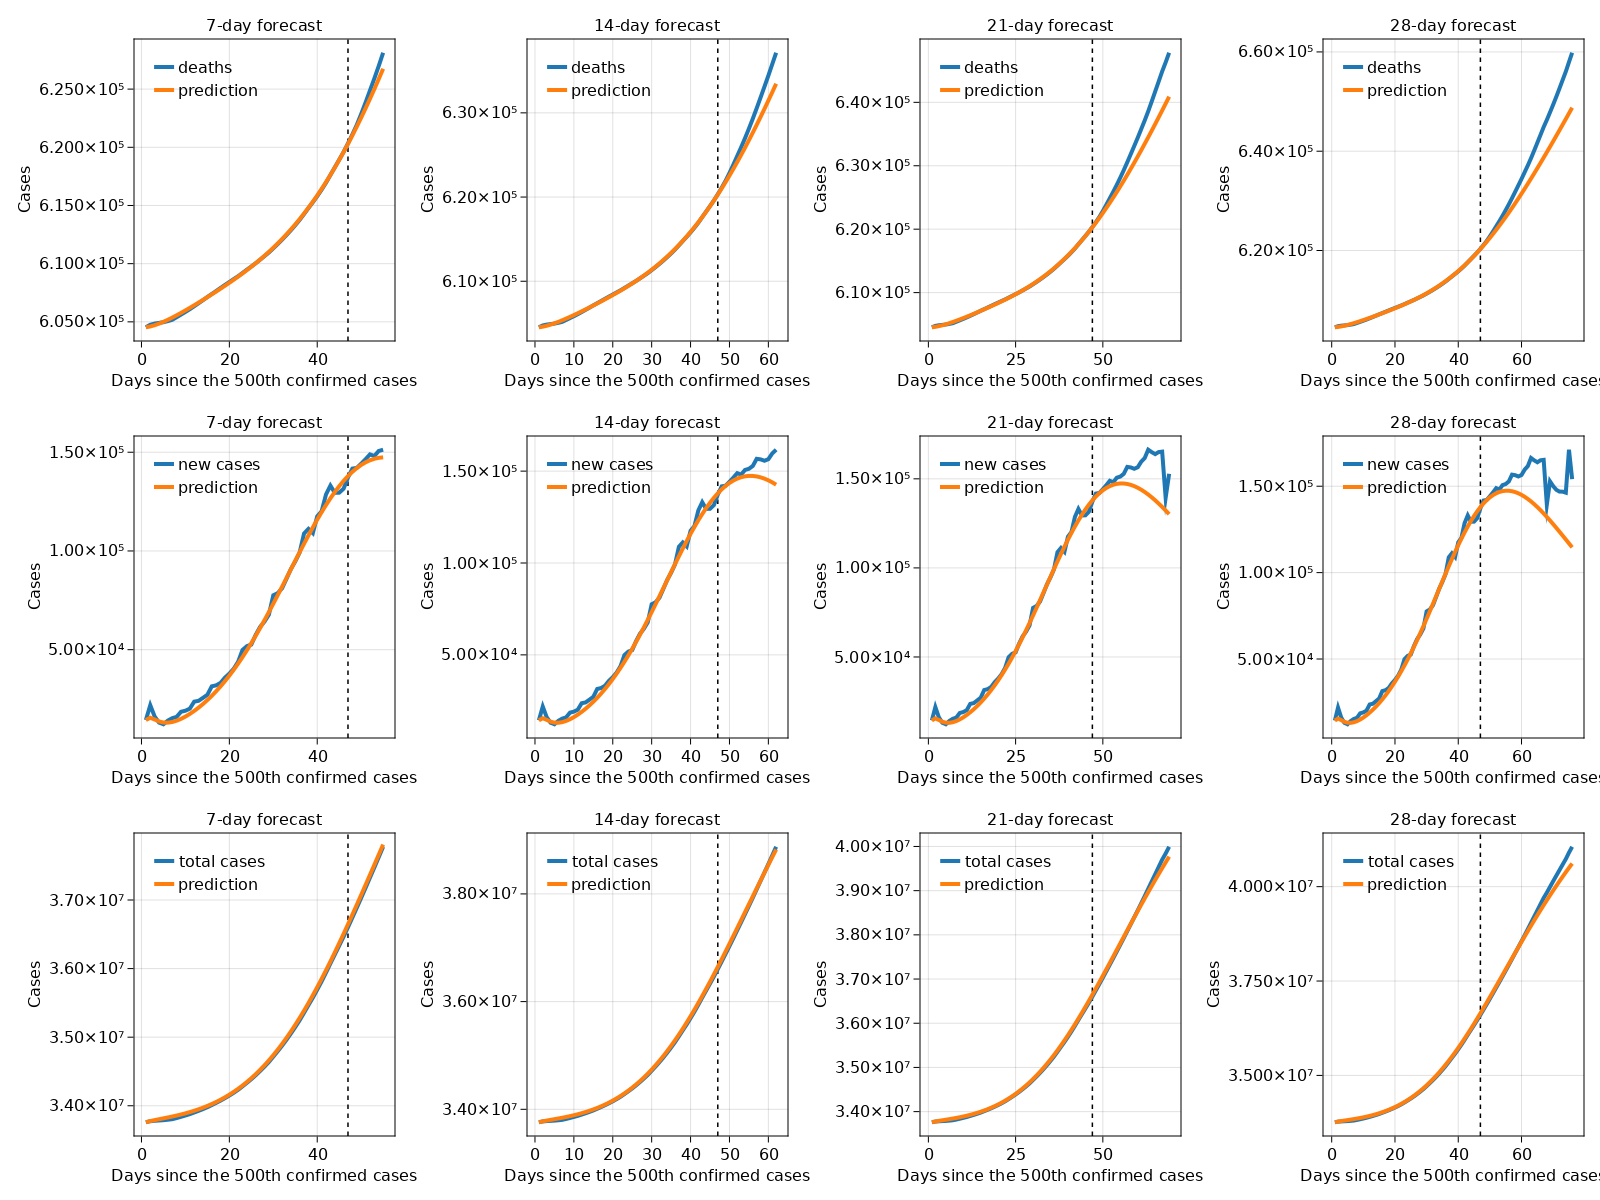
\includegraphics[scale=0.25]{baseline/unitedstates/20211216125000.baseline.unitedstates.forecasts.png}
    \caption{Predictions made by the baseline model after having trained with data for the United States. The black vertical dashed line marks the last day in the training period.}
    \label{fig:predictions-usa-baseline}
\end{figure}

\begin{figure}[!htb]
    \centering
    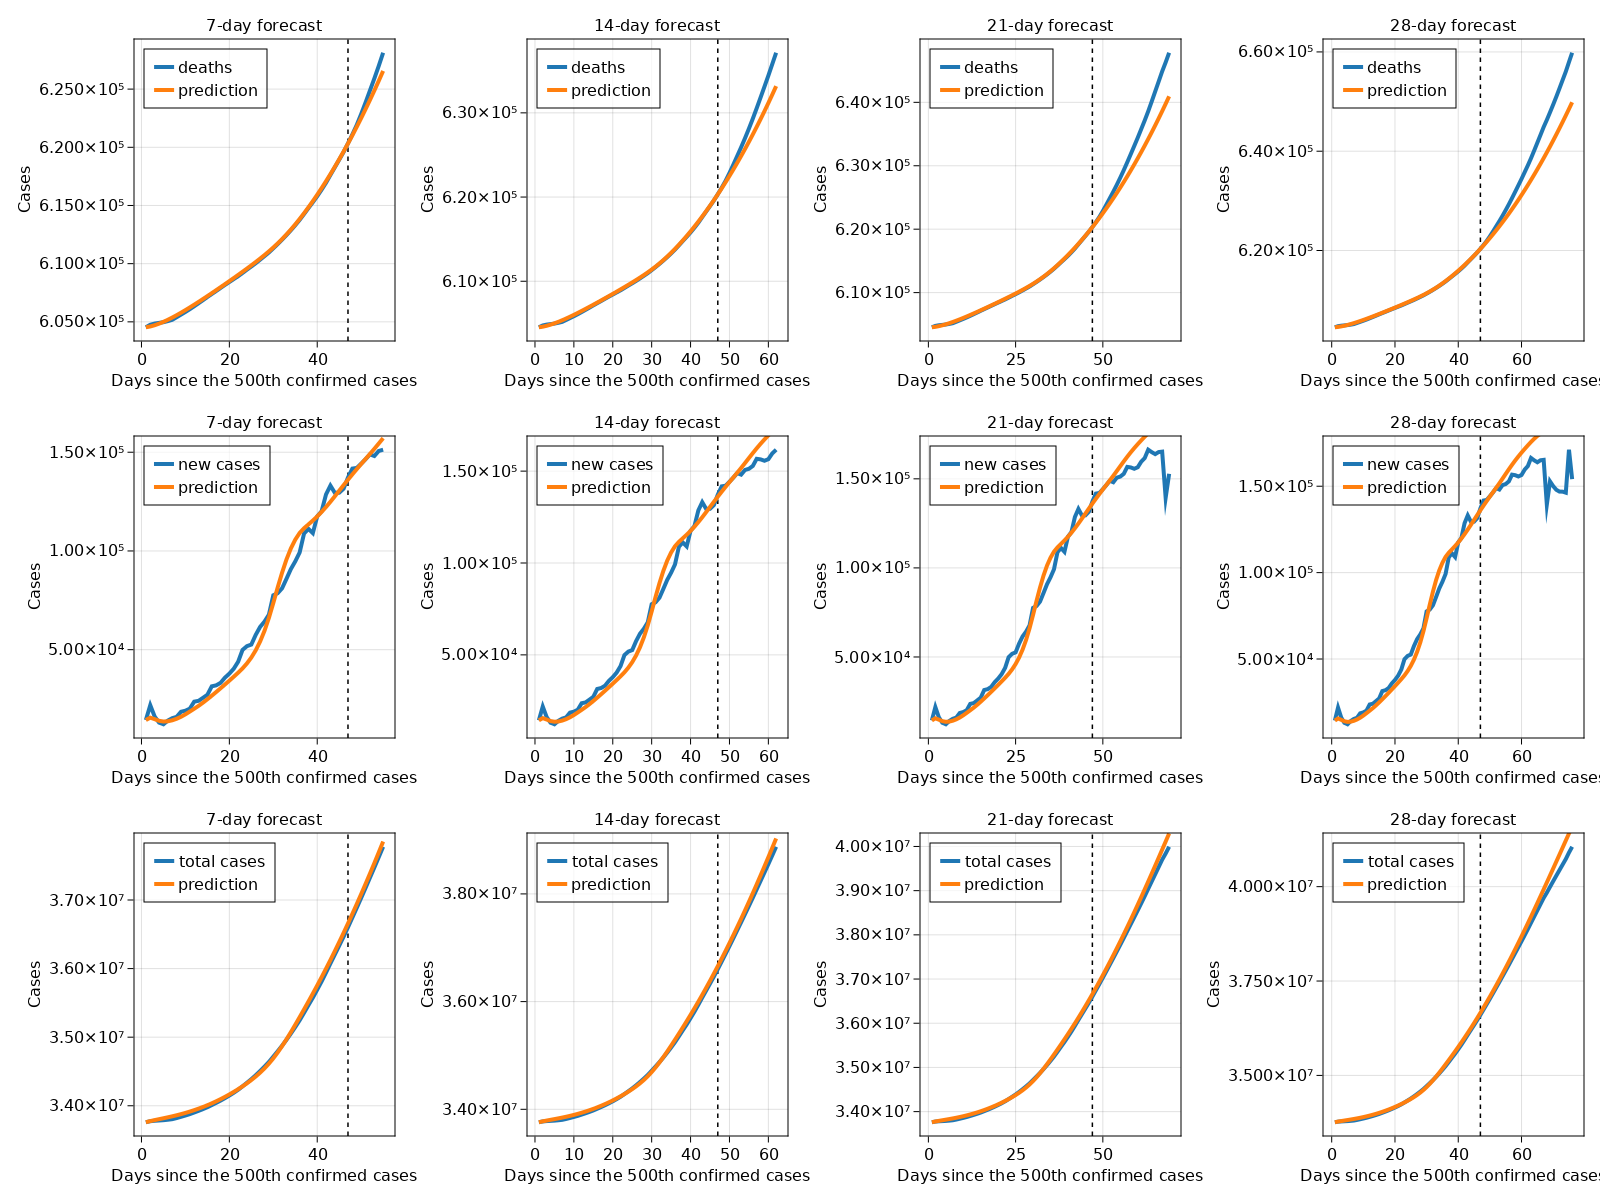
\includegraphics[scale=0.25]{fb1/unitedstates/20211216233634.fbmobility1.unitedstates.forecasts.png}
    \caption{Predictions made by the second version of the model that uses Facebook's Movement Range Maps dataset after having trained with data for the United States. The black vertical dashed line marks the last day in the training period.}
    \label{fig:predictions-usa-fb1}
\end{figure}

% LOS ANGELES

\begin{figure}[!htb]
    \centering
    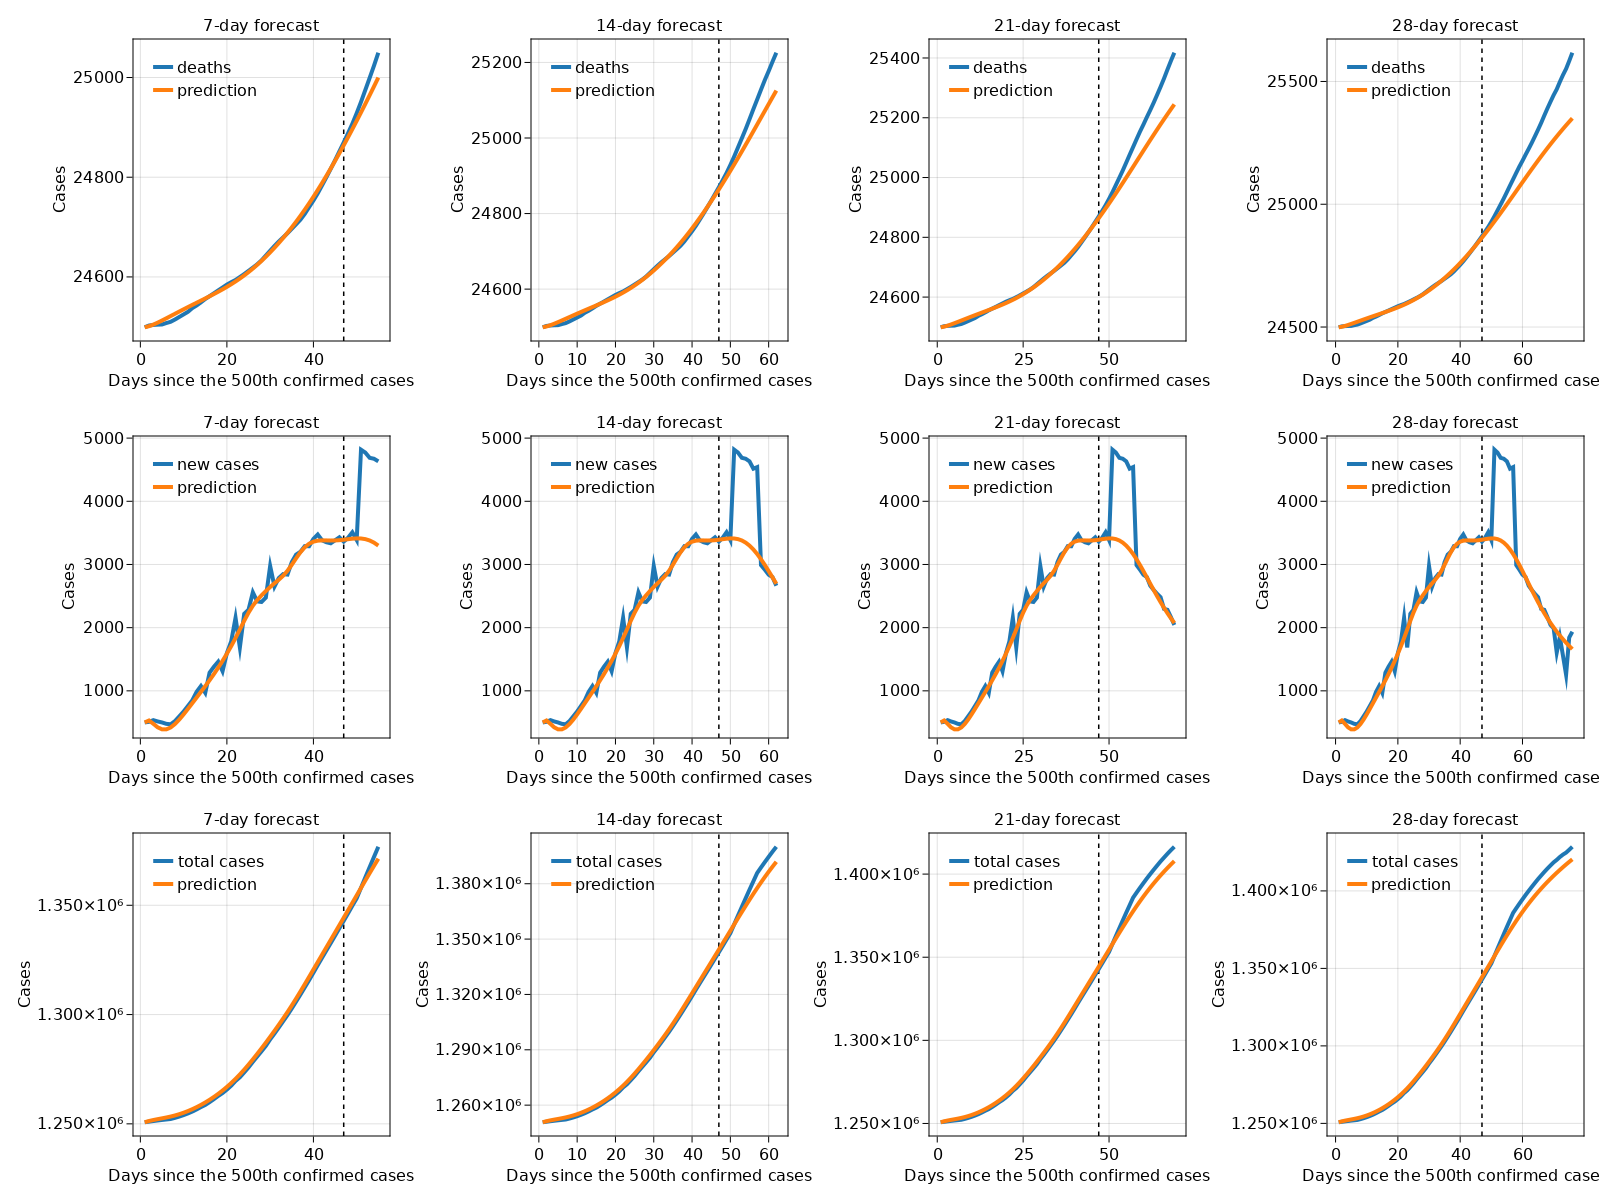
\includegraphics[scale=0.25]{baseline/losangeles_ca/20211216124108.baseline.losangeles_ca.forecasts.png}
    \caption{Predictions made by the baseline model after having trained with data for Los Angeles, California. The black vertical dashed line marks the last day in the training period.}
    \label{fig:predictions-losangeles-baseline}
\end{figure}

\begin{figure}[!htb]
    \centering
    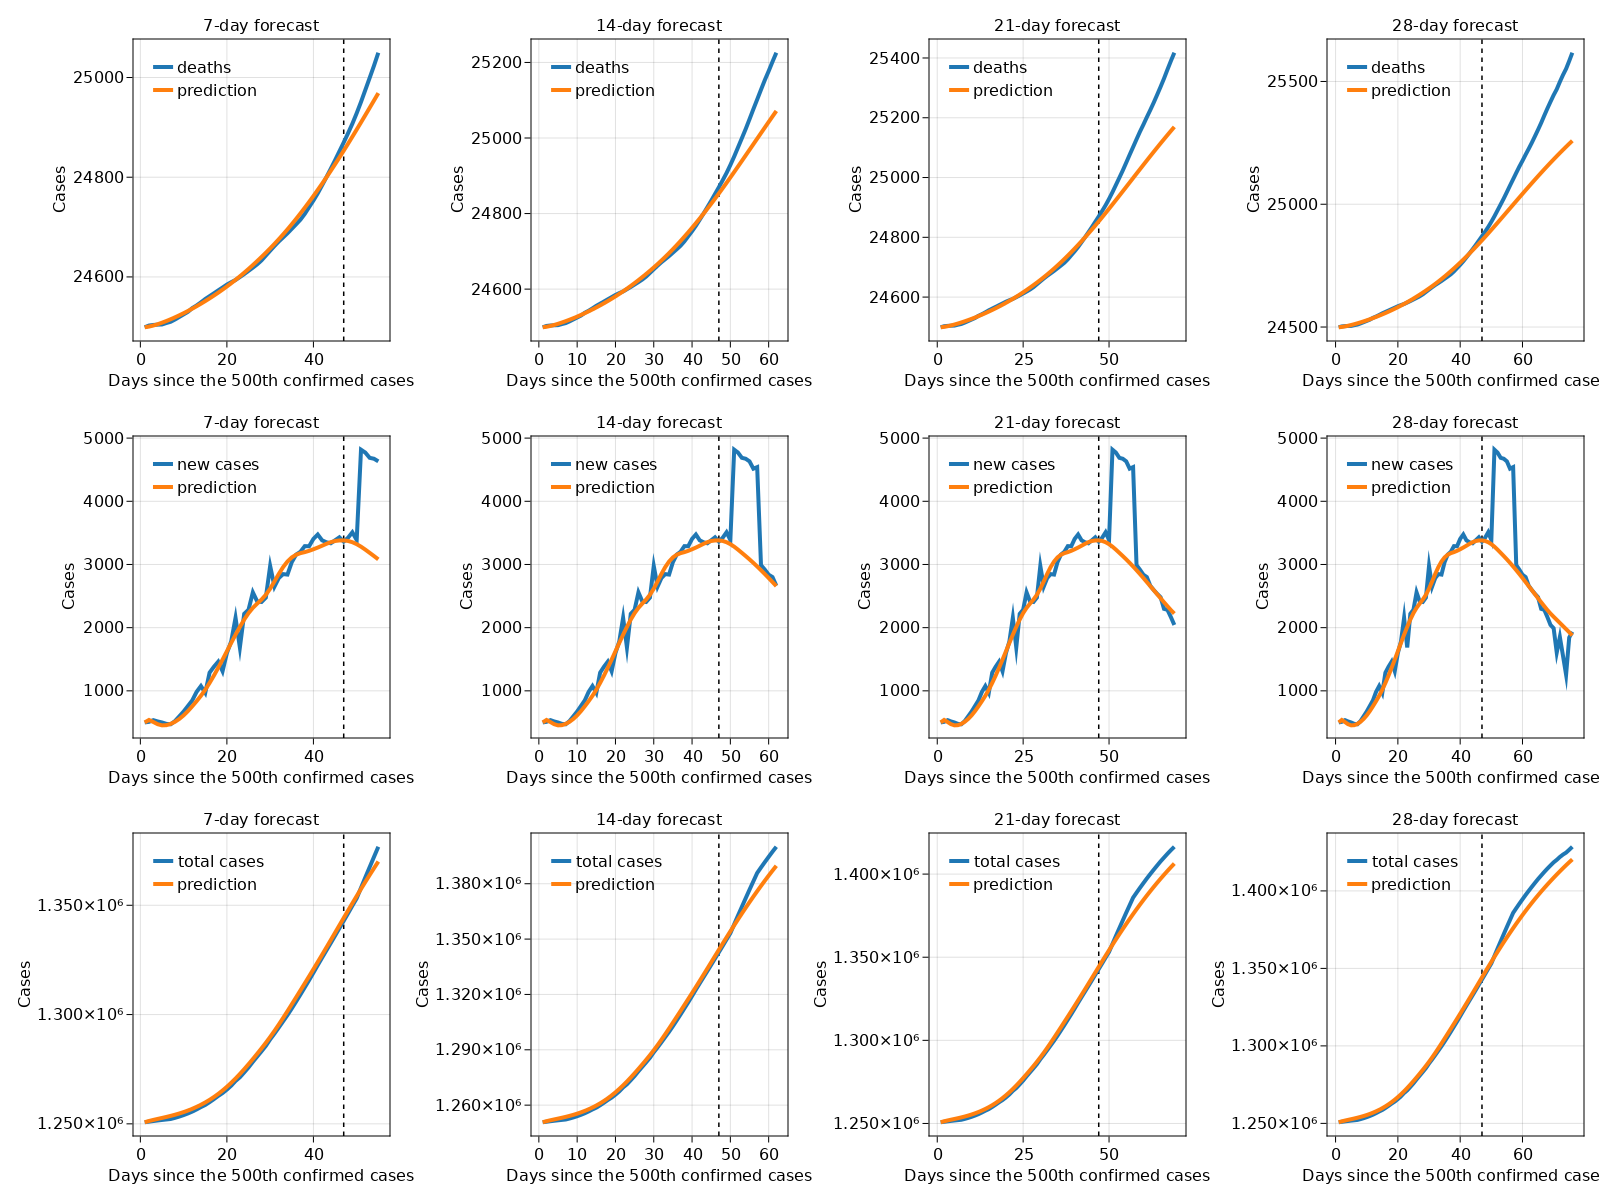
\includegraphics[scale=0.25]{fb1/losangeles_ca/20211216180602.fbmobility1.losangeles_ca.forecasts.png}
    \caption{Predictions made by the second version of the model that uses Facebook's Movement Range Maps dataset after having trained with data for Los Angeles, California. The black vertical dashed line marks the last day in the training period.}
    \label{fig:predictions-losangeles-fb1}
\end{figure}

\begin{figure}[!htb]
    \centering
    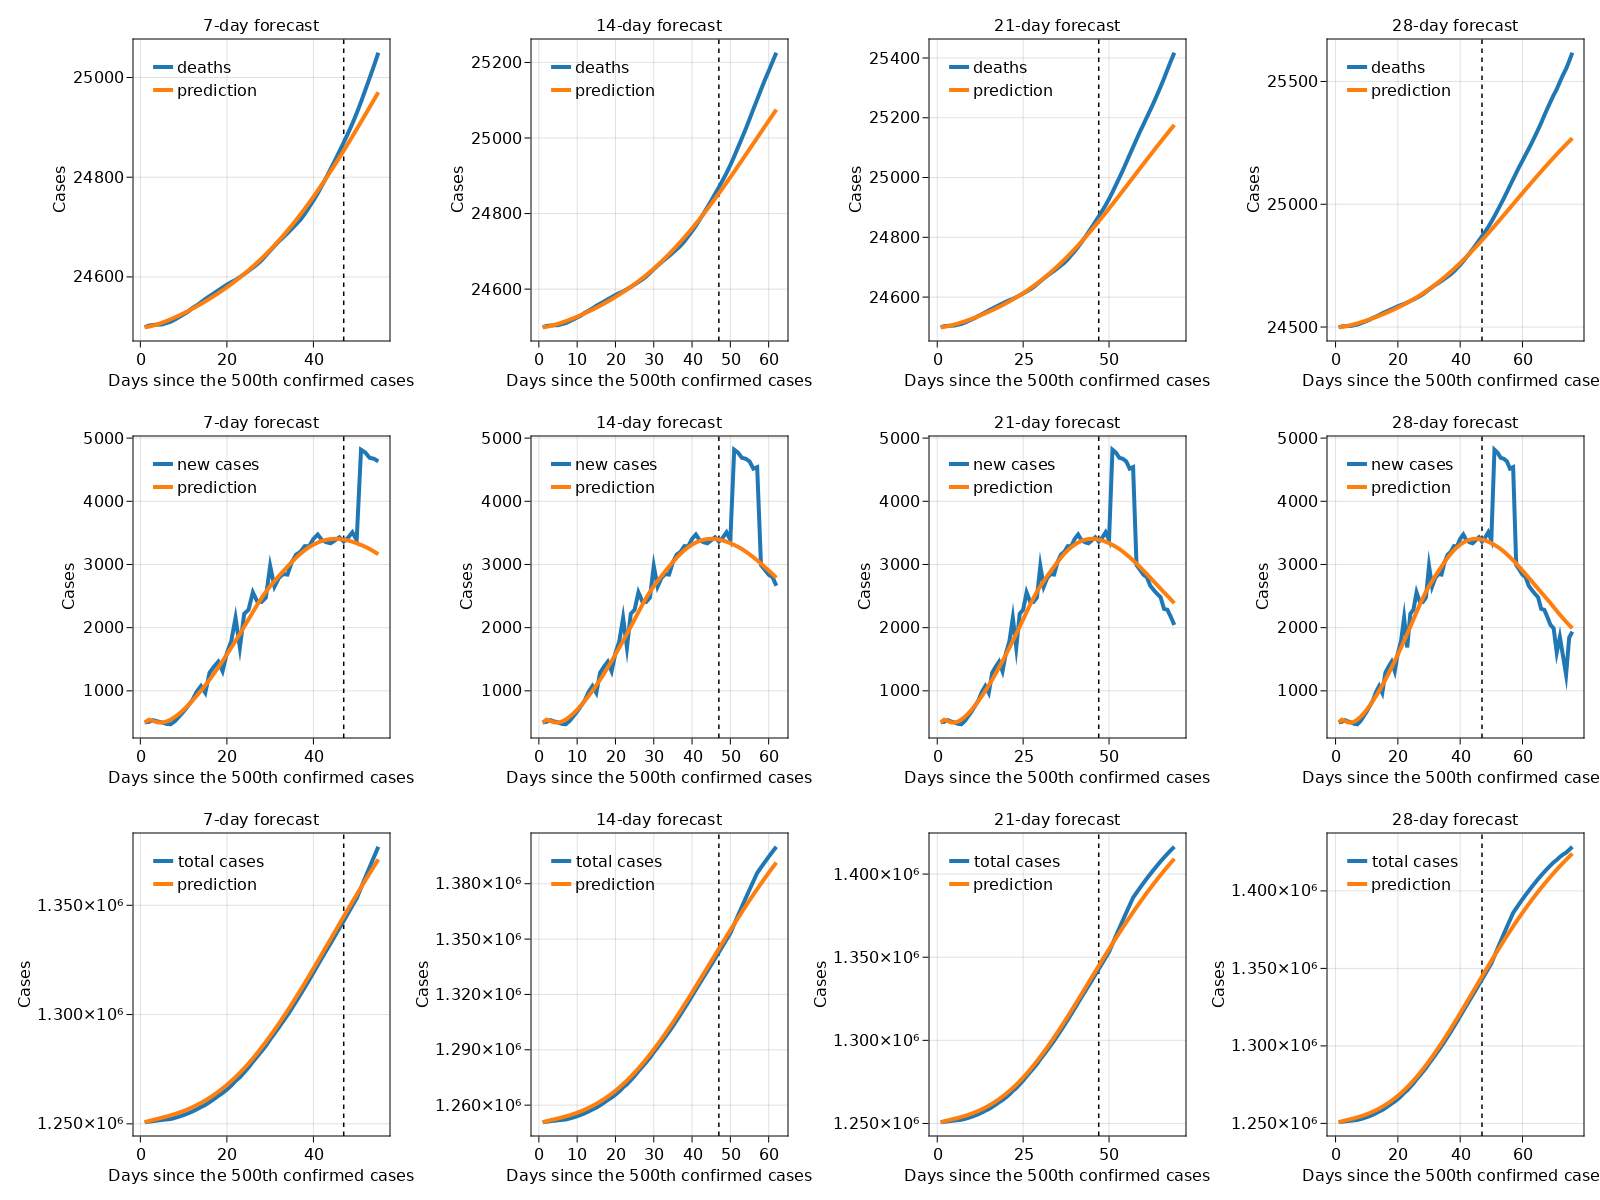
\includegraphics[scale=0.25]{fb2/losangeles_ca/20211216142727.fbmobility2.losangeles_ca.forecasts.png}
    \caption{Predictions made by the second version of the model that uses Facebook's Movement Range Maps dataset and Social Proximity to Cases Index after having trained with data for Los Angeles, California. The black vertical dashed line marks the last day in the training period.}
    \label{fig:predictions-losangeles-fb2}
\end{figure}

% HARRIS

\begin{figure}[!htb]
    \centering
    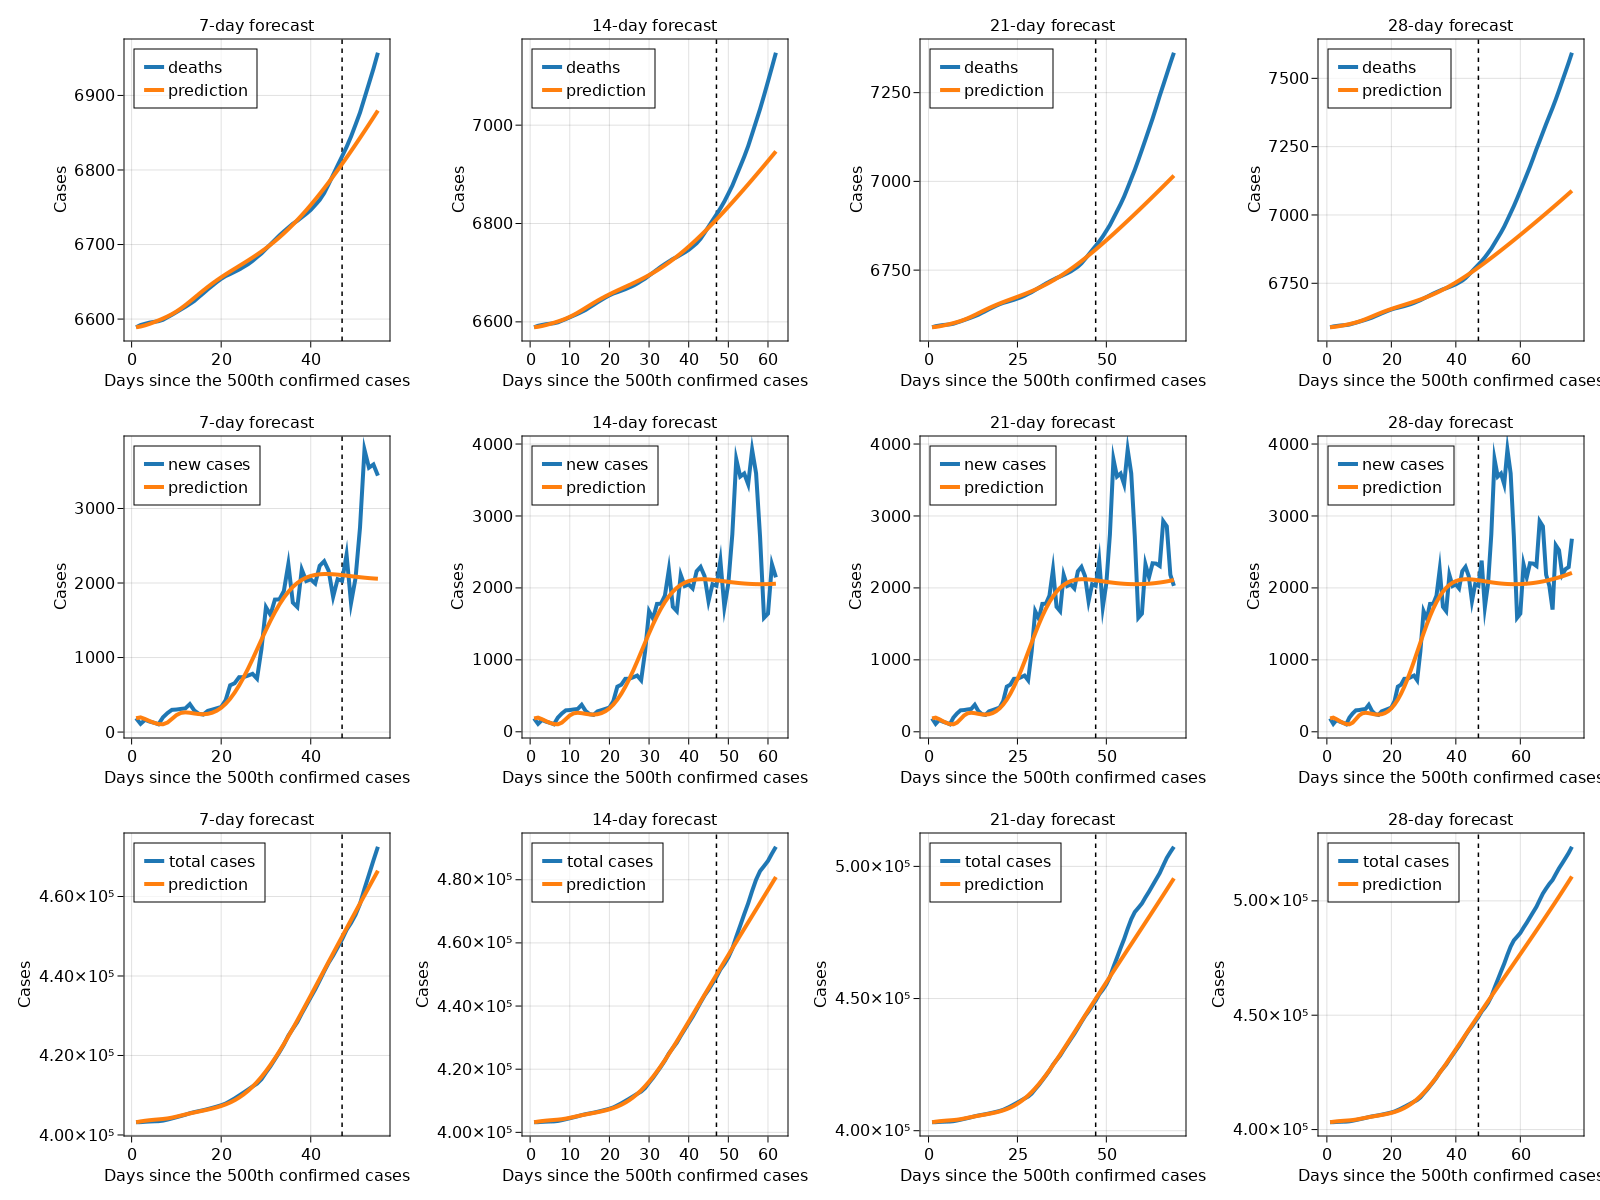
\includegraphics[scale=0.25]{baseline/harris_tx/20211216154445.baseline.harris_tx.forecasts.png}
    \caption{Predictions made by the baseline model after having trained with data for Harris, Texas. The black vertical dashed line marks the last day in the training period.}
    \label{fig:predictions-harris-baseline}
\end{figure}

\begin{figure}[!htb]
    \centering
    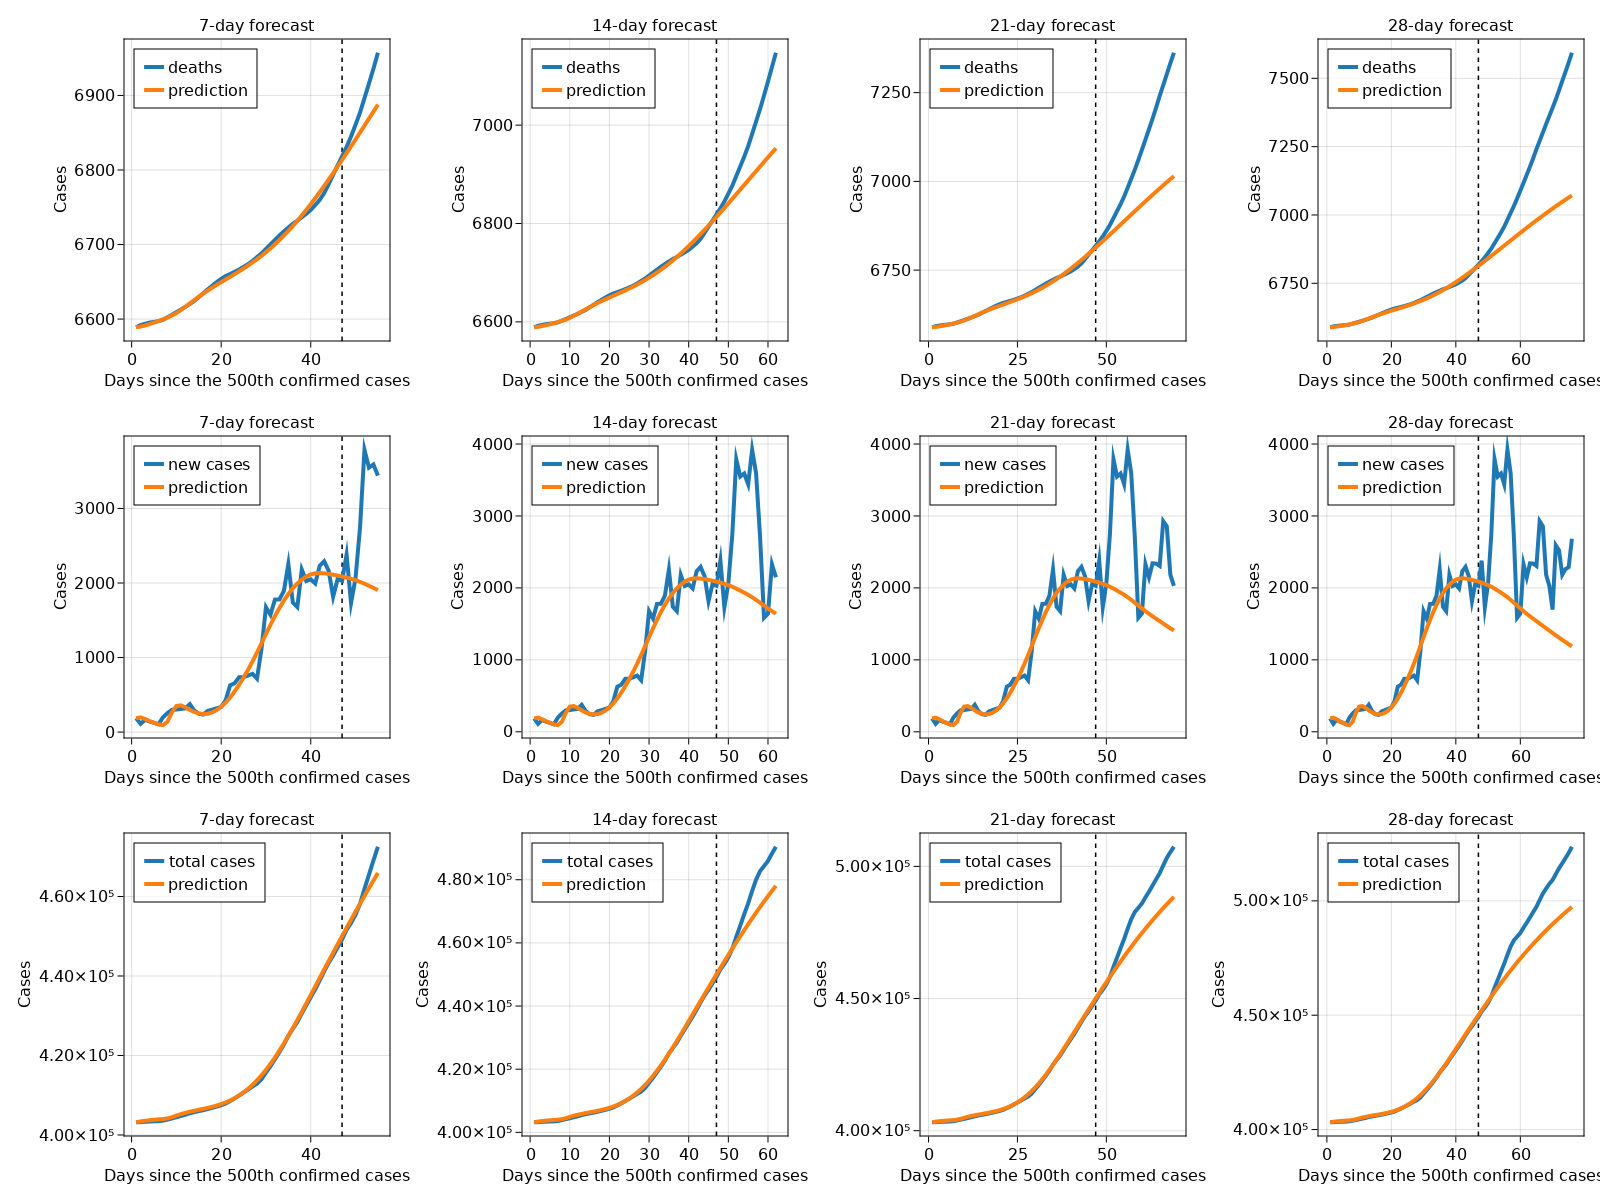
\includegraphics[scale=0.25]{fb1/harris_tx/20211216231719.fbmobility1.harris_tx.forecasts.png}
    \caption{Predictions made by the second version of the model that uses Facebook's Movement Range Maps dataset after having trained with data for Harris, Texas. The black vertical dashed line marks the last day in the training period.}
    \label{fig:predictions-harris-fb1}
\end{figure}

\begin{figure}[!htb]
    \centering
    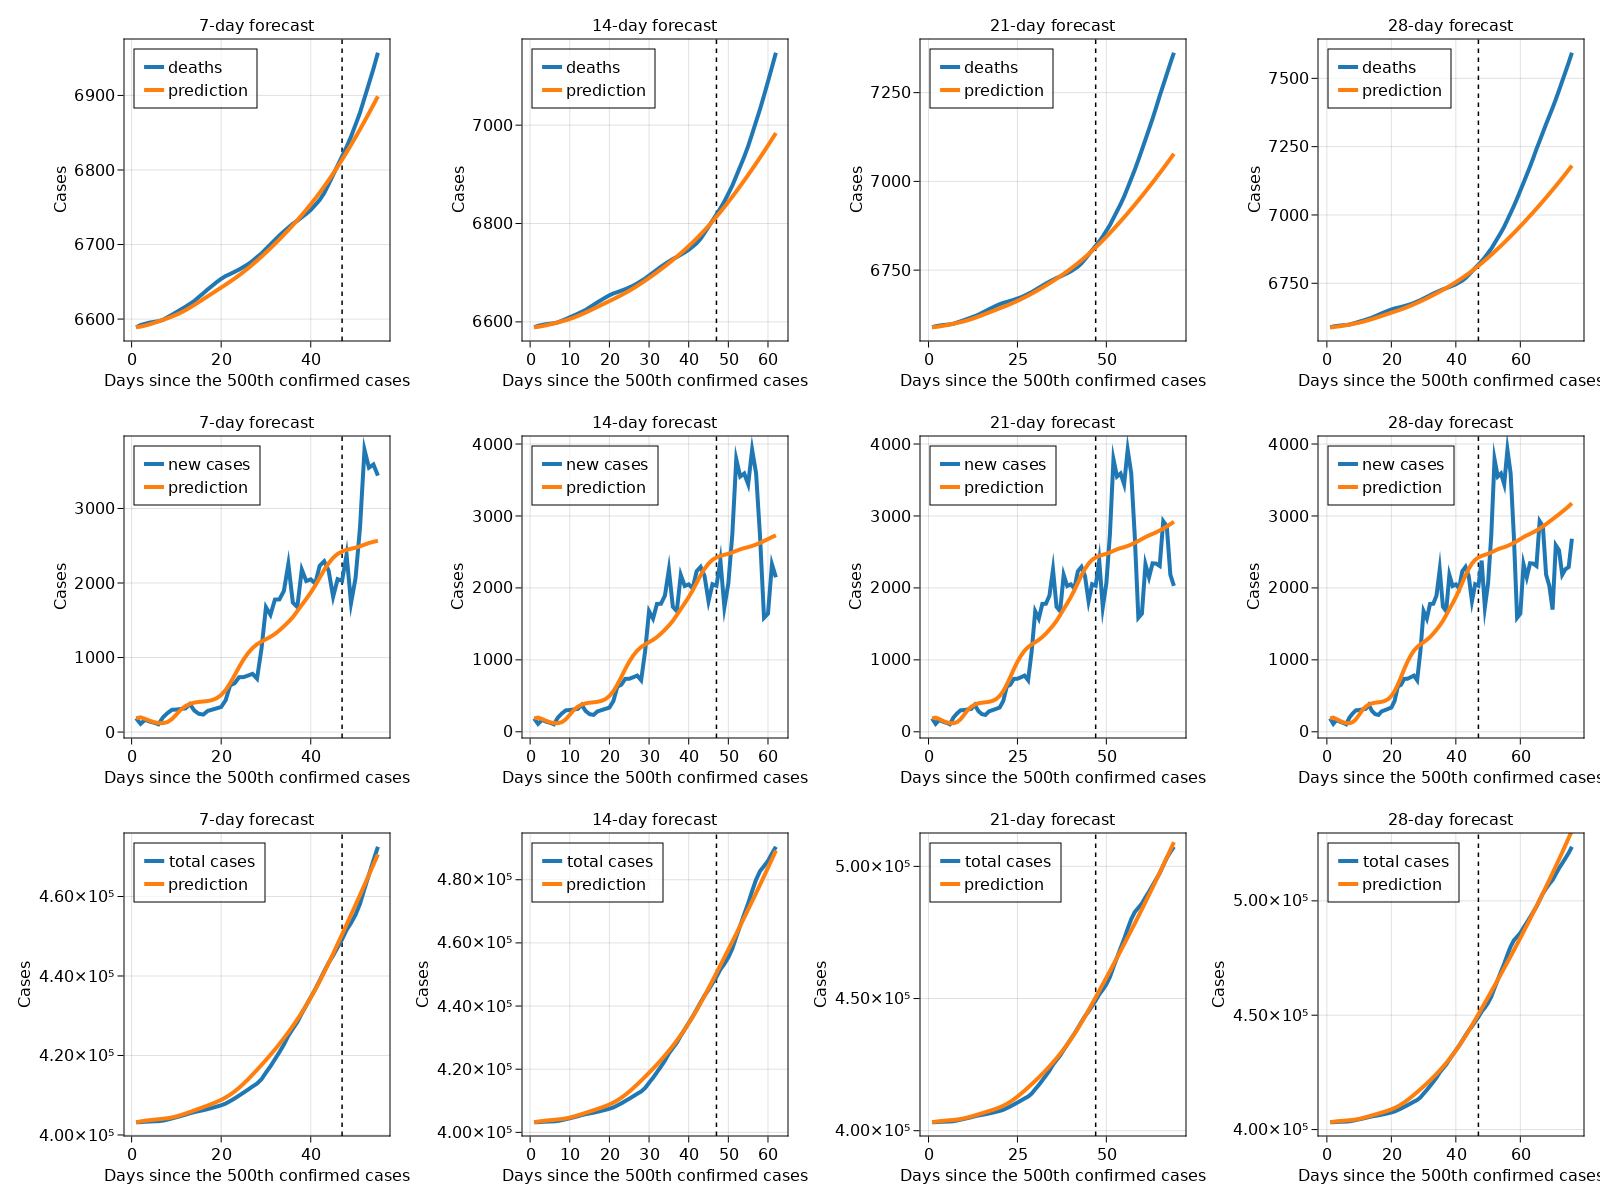
\includegraphics[scale=0.25]{fb2/harris_tx/20211217204936.fbmobility2.harris_tx.forecasts.png}
    \caption{Predictions made by the second version of the model that uses Facebook's Movement Range Maps dataset and Social Proximity to Cases Index after having trained with data for Harris, Texas. The black vertical dashed line marks the last day in the training period.}
    \label{fig:predictions-harris-fb2}
\end{figure}

% COOK

\begin{figure}[!htb]
    \centering
    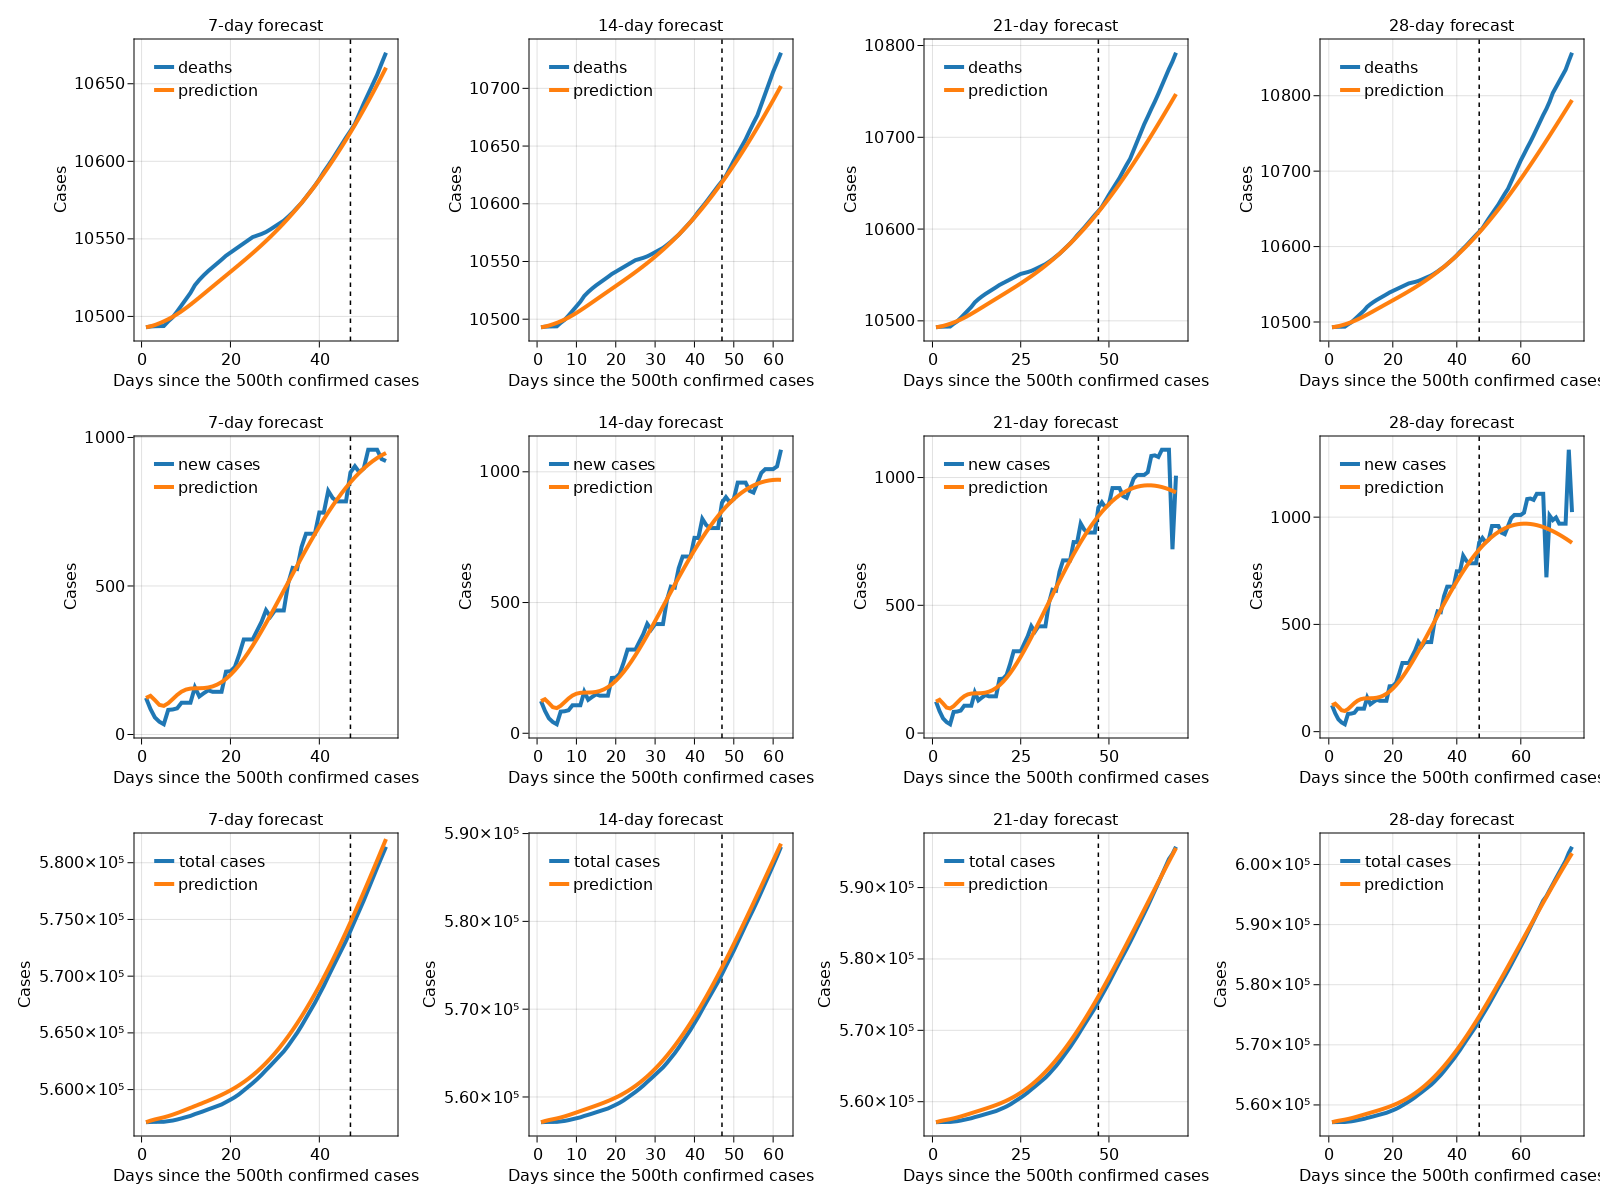
\includegraphics[scale=0.25]{baseline/cook_il/20211215163025.baseline.cook_il.forecasts.png}
    \caption{Predictions made by the baseline model after having trained with data for Cook, Illinois. The black vertical dashed line marks the last day in the training period.}
    \label{fig:predictions-cook-baseline}
\end{figure}

\begin{figure}[!htb]
    \centering
    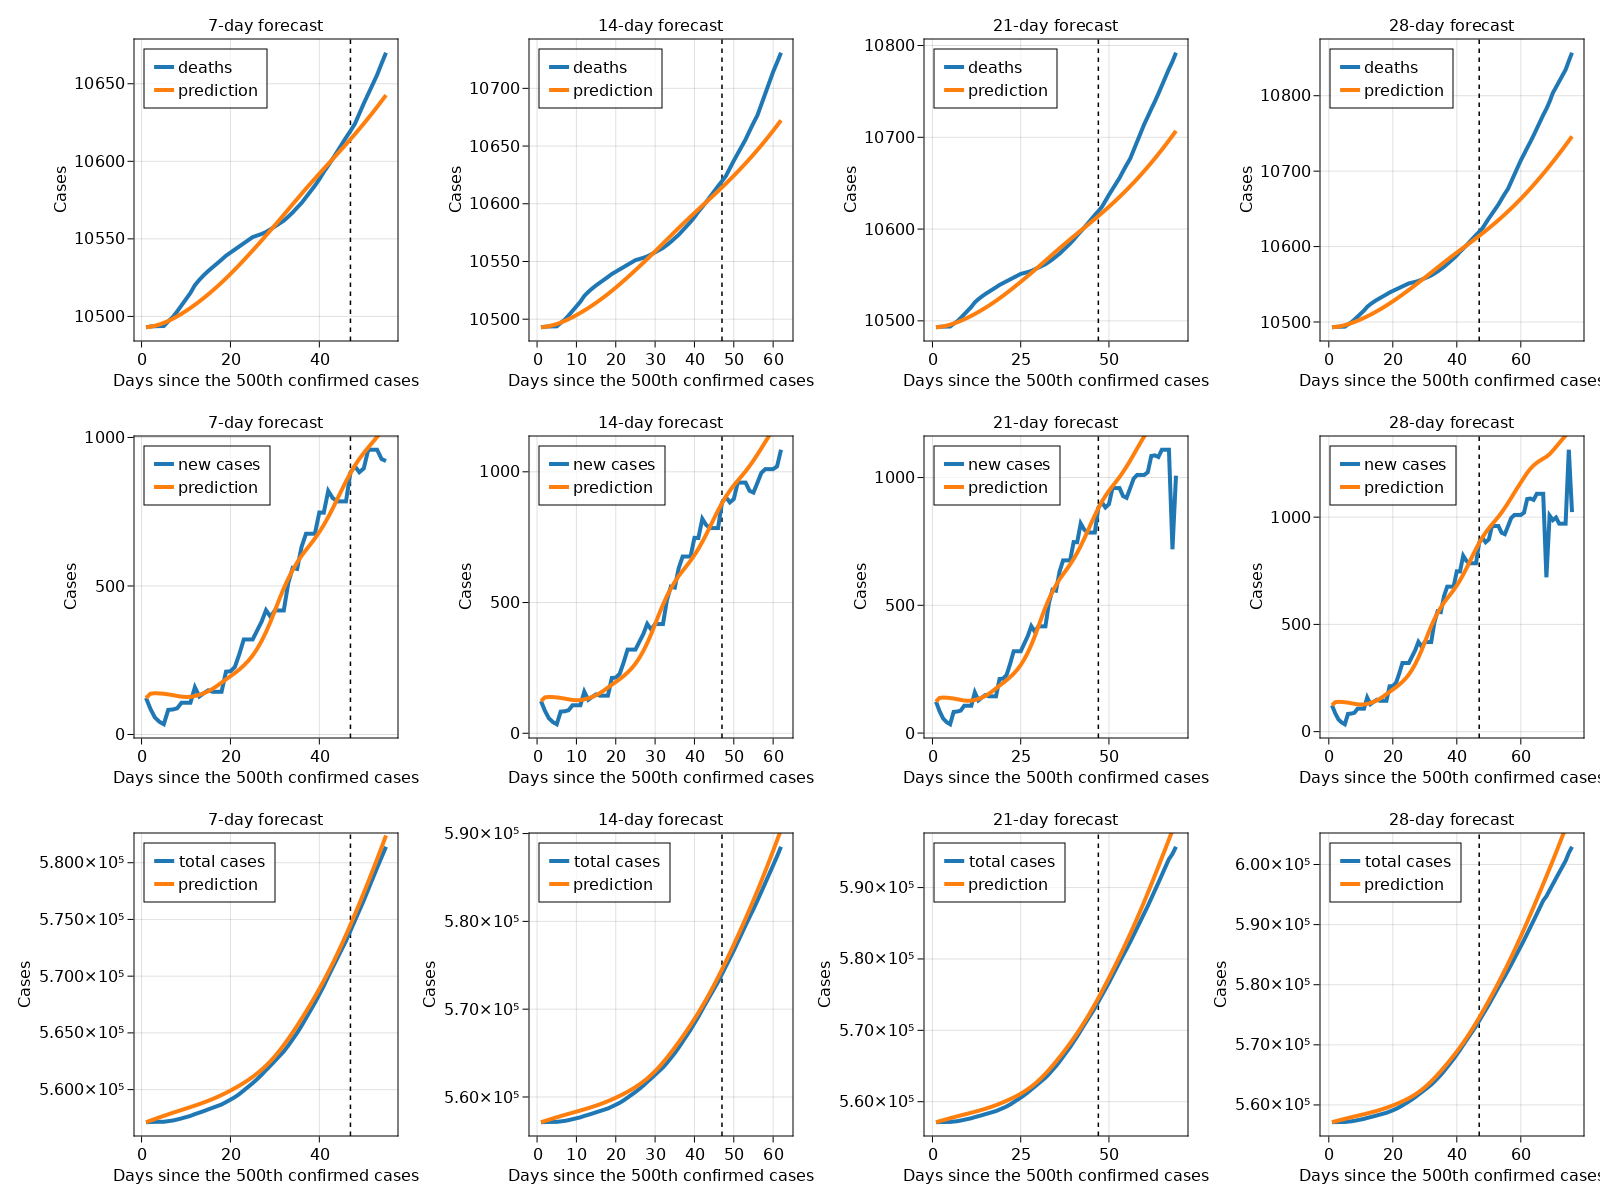
\includegraphics[scale=0.25]{fb1/cook_il/20211216131821.fbmobility1.cook_il.forecasts.png}
    \caption{Predictions made by the second version of the model that uses Facebook's Movement Range Maps dataset after having trained with data for Cook, Illinois. The black vertical dashed line marks the last day in the training period.}
    \label{fig:predictions-cook-fb1}
\end{figure}

\begin{figure}[!htb]
    \centering
    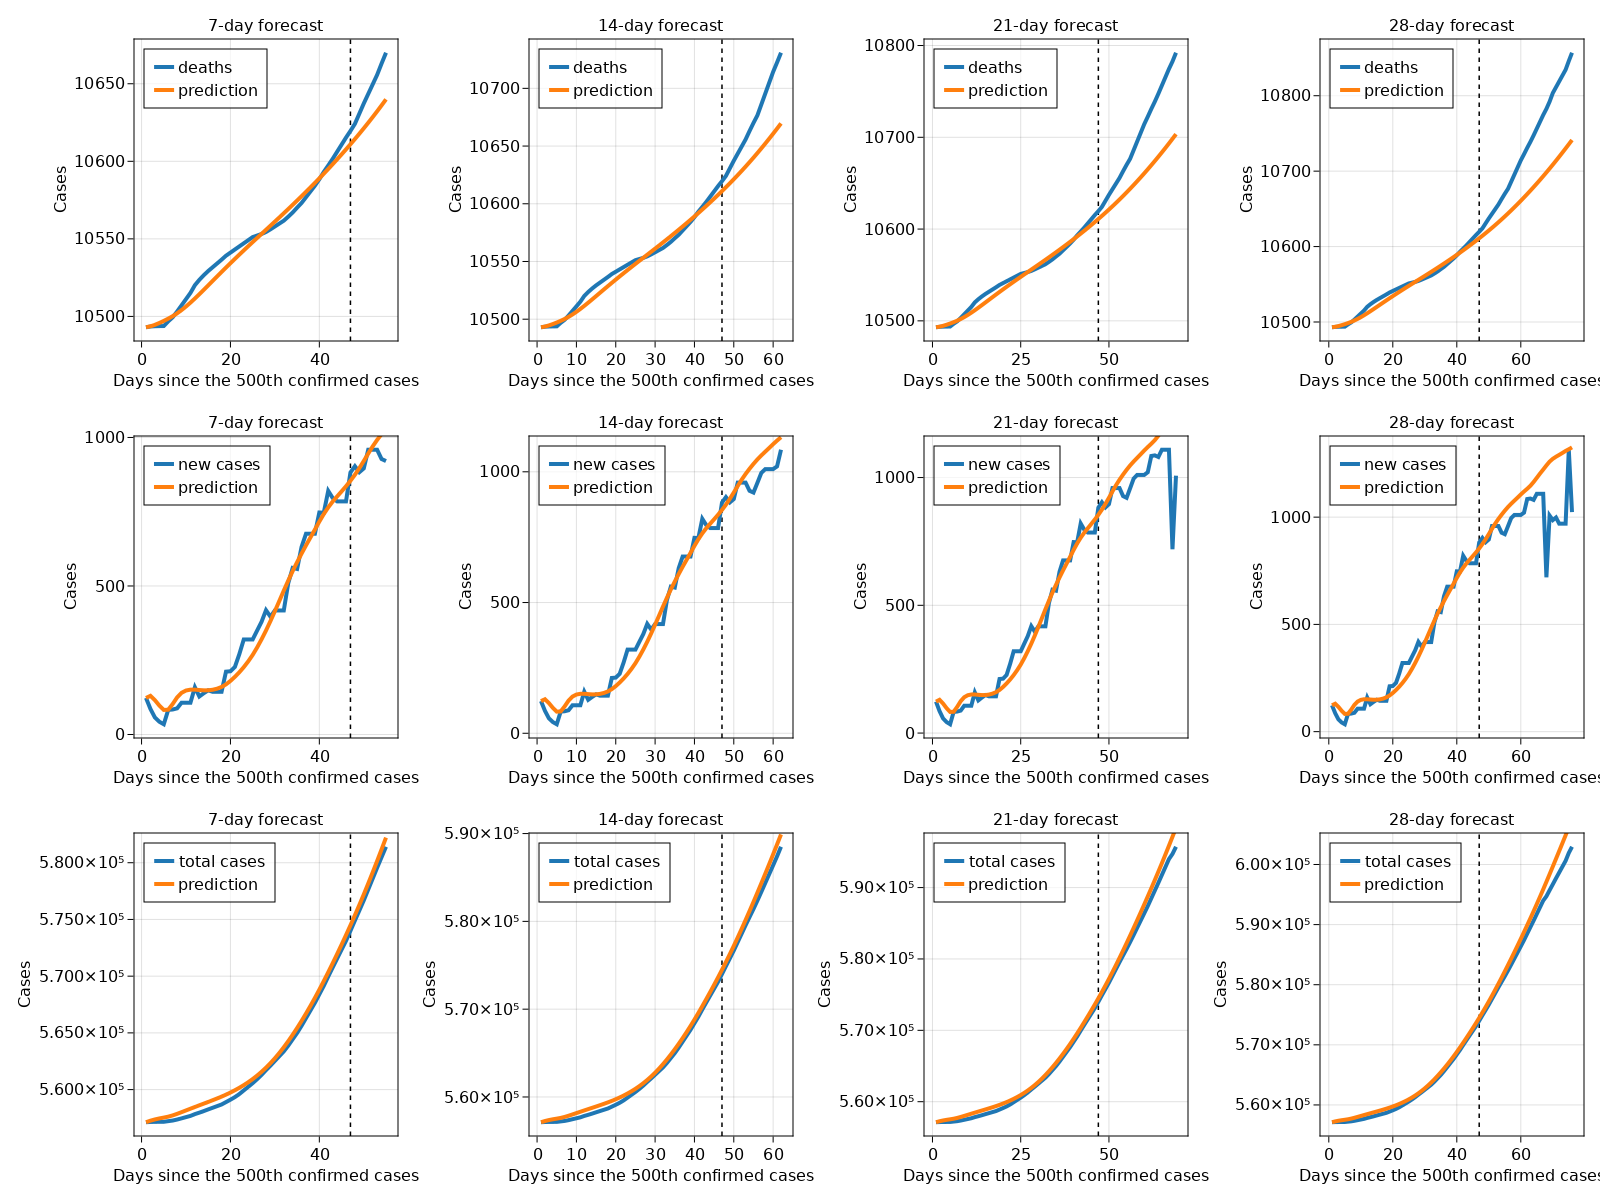
\includegraphics[scale=0.25]{fb2/cook_il/20211216142727.fbmobility2.cook_il.forecasts.png}
    \caption{Predictions made by the second version of the model that uses Facebook's Movement Range Maps dataset and Social Proximity to Cases Index after having trained with data for Cook, Illinois. The black vertical dashed line marks the last day in the training period.}
    \label{fig:predictions-cook-fb2}
\end{figure}

% MARICOPA

\begin{figure}[!htb]
    \centering
    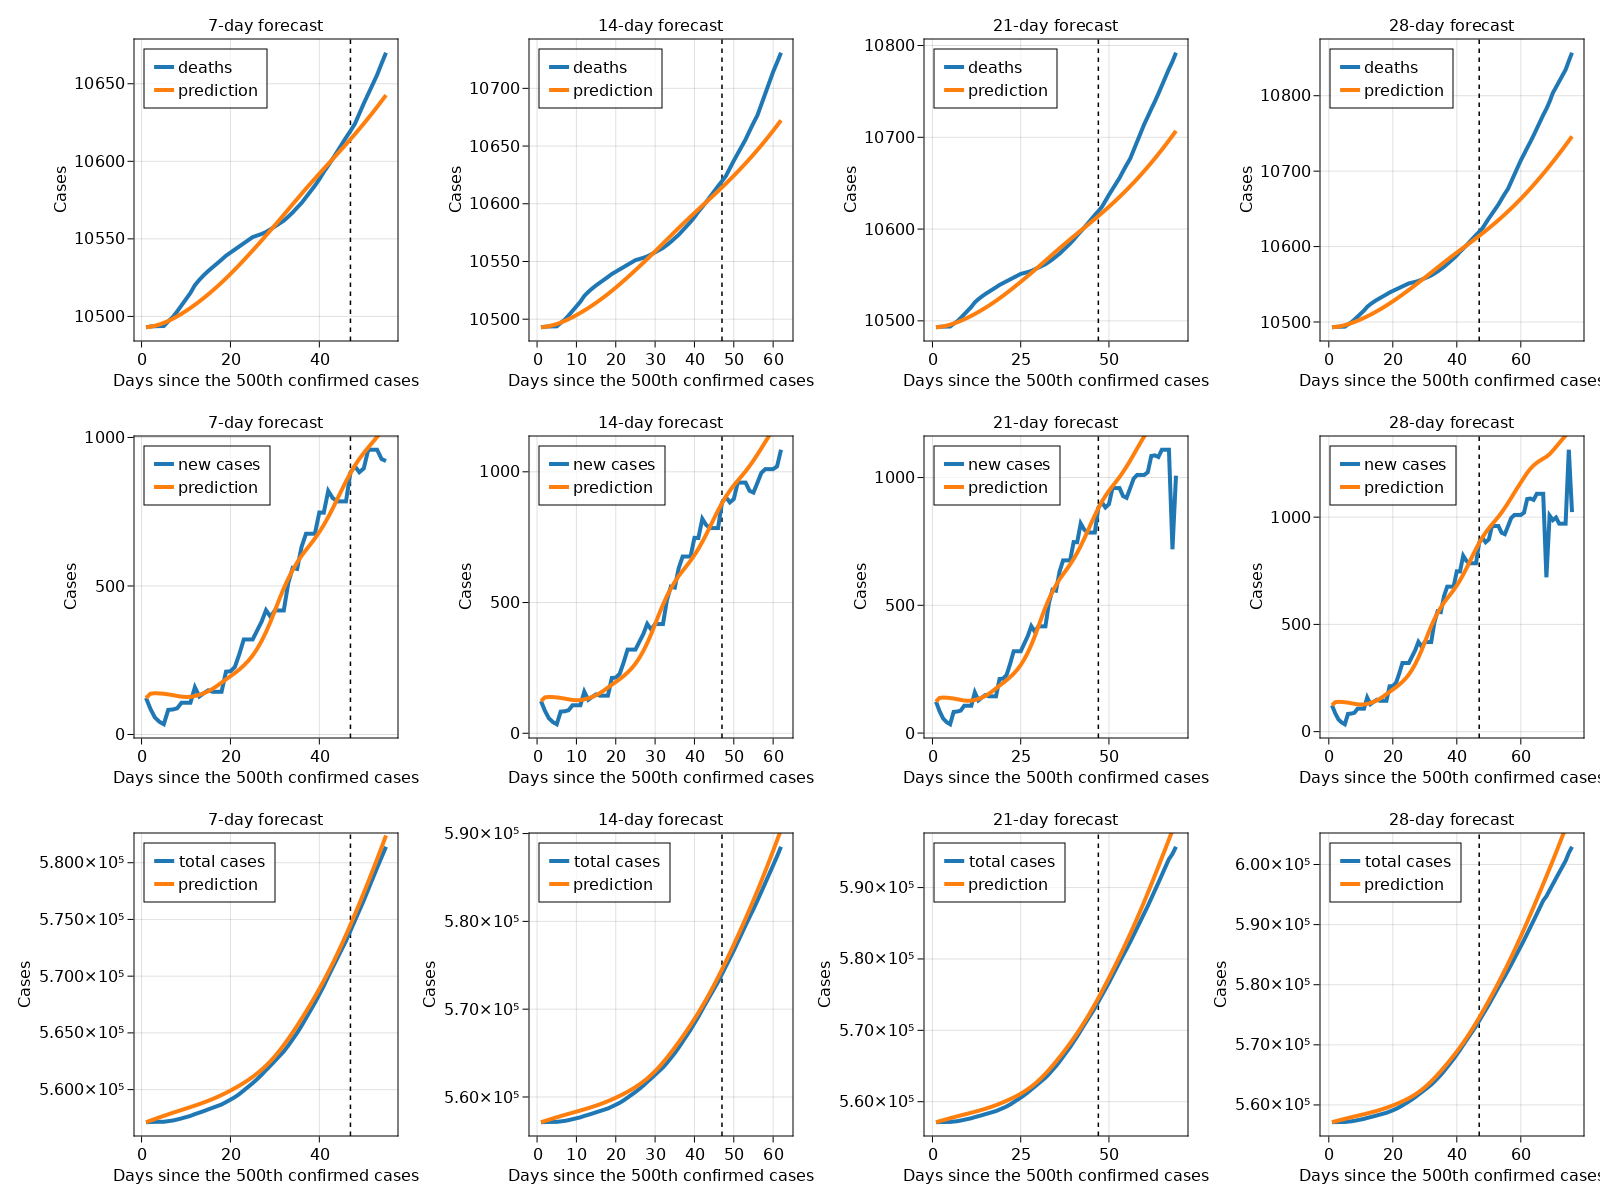
\includegraphics[scale=0.25]{fb1/cook_il/20211216131821.fbmobility1.cook_il.forecasts.png}
    \caption{Predictions made by the baseline model after having trained with data for Maricopa, Arizona. The black vertical dashed line marks the last day in the training period.}
    \label{fig:predictions-maricopa-baseline}
\end{figure}

\begin{figure}[!htb]
    \centering
    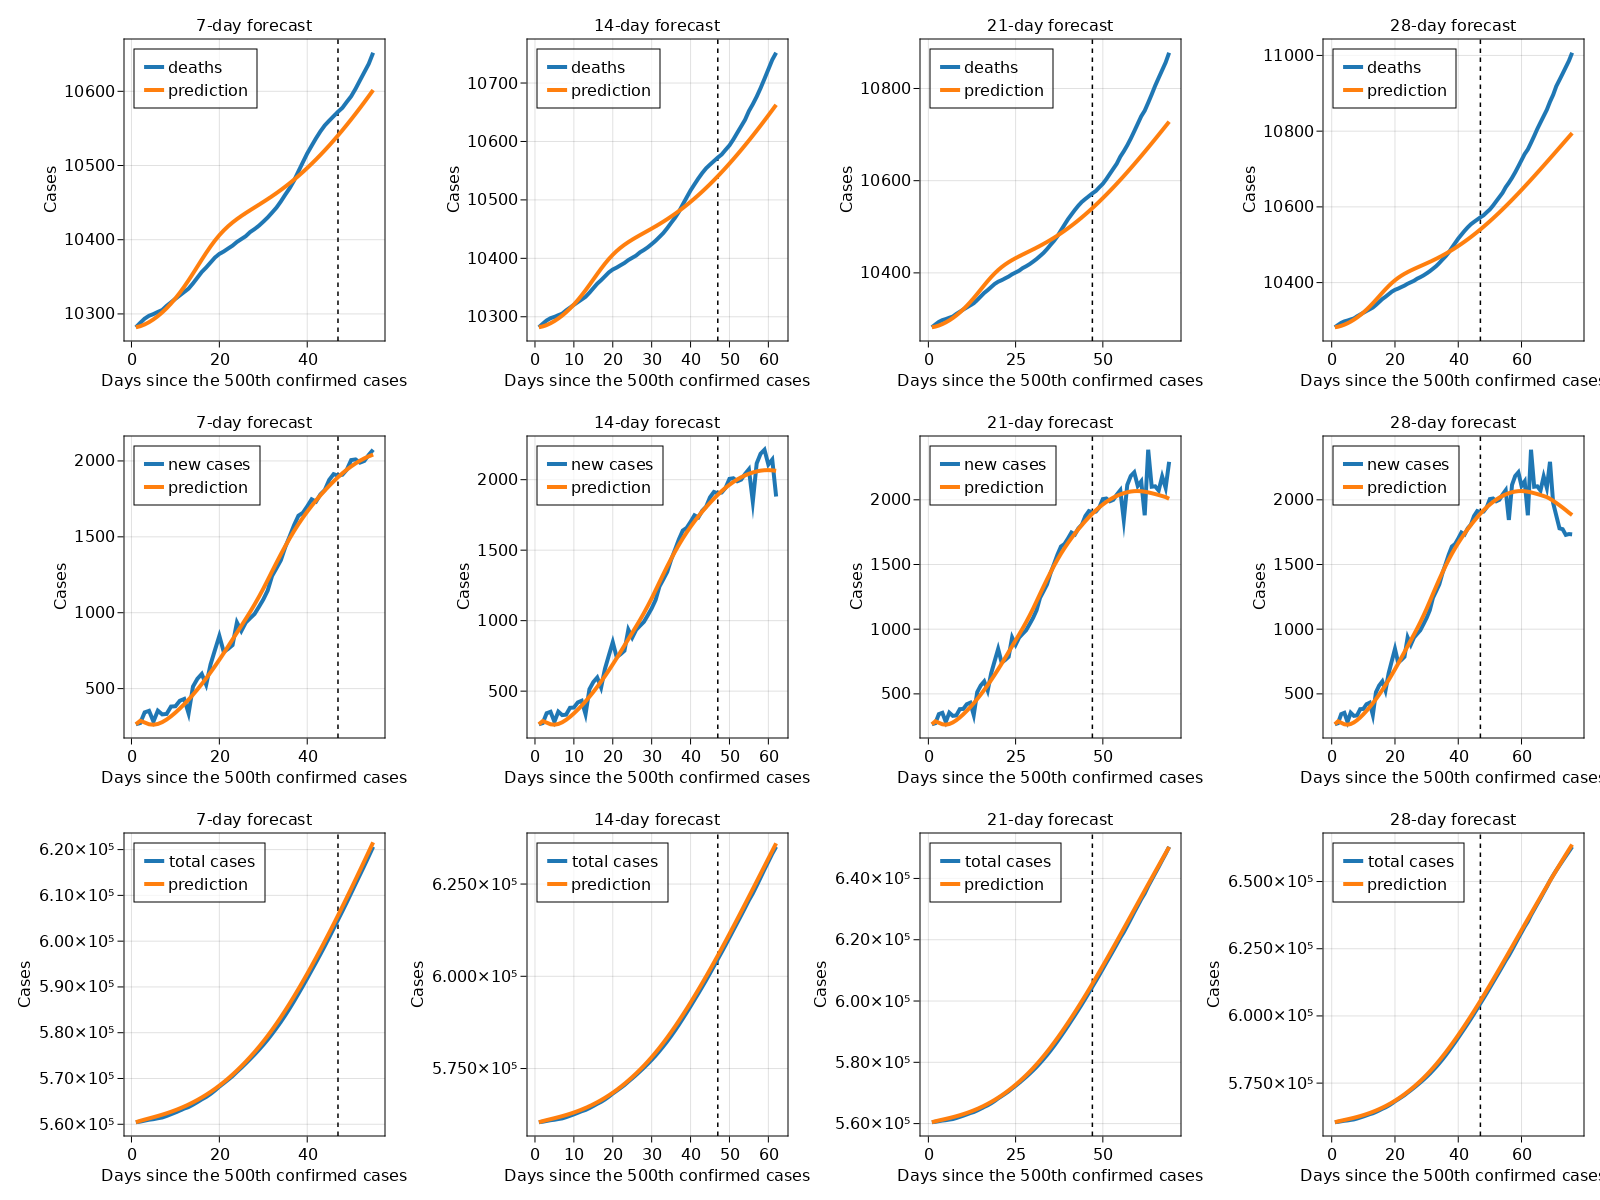
\includegraphics[scale=0.25]{fb1/maricopa_az/20211216131821.fbmobility1.maricopa_az.forecasts.png}
    \caption{Predictions made by the second version of the model that uses Facebook's Movement Range Maps dataset after having trained with data for Maricopa, Arizona. The black vertical dashed line marks the last day in the training period.}
    \label{fig:predictions-maricopa-fb1}
\end{figure}

\begin{figure}[!htb]
    \centering
    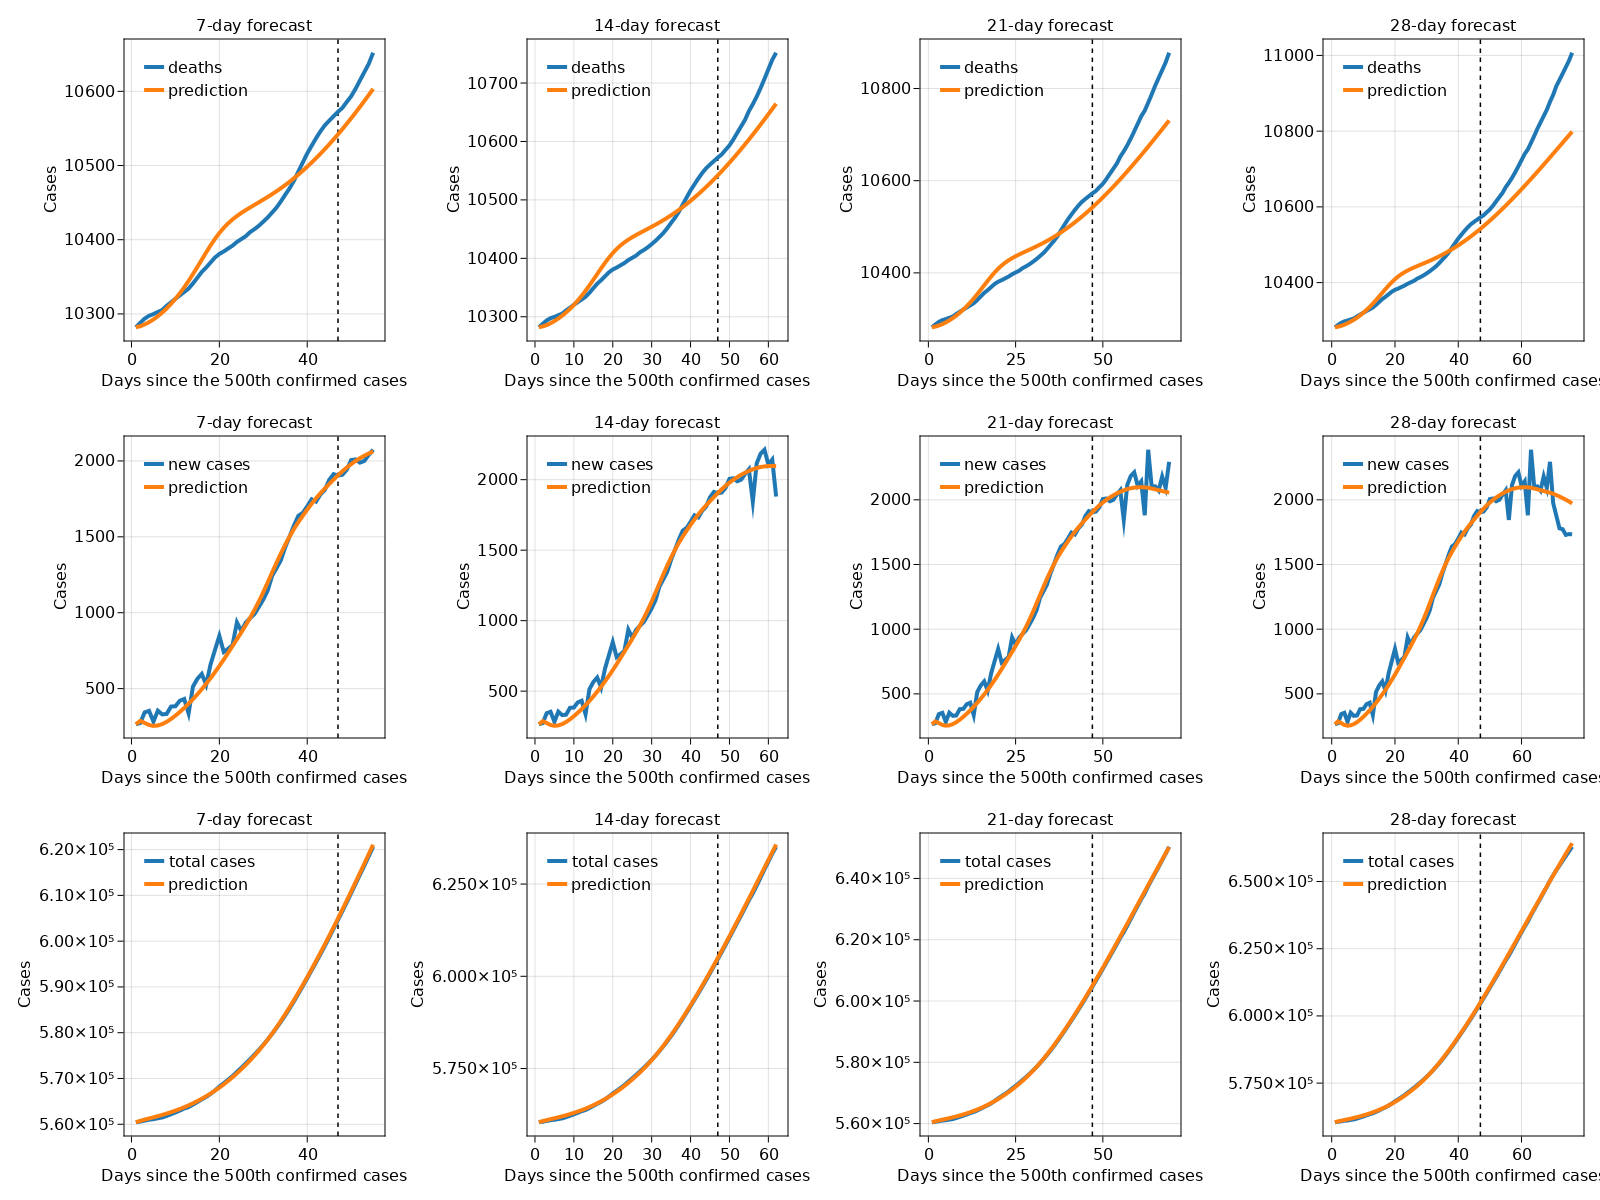
\includegraphics[scale=0.25]{fb2/maricopa_az/20211216193717.fbmobility2.maricopa_az.forecasts.png}
    \caption{Predictions made by the second version of the model that uses Facebook's Movement Range Maps dataset and Social Proximity to Cases Index after having trained with data for Maricopa, Arizona. The black vertical dashed line marks the last day in the training period.}
    \label{fig:predictions-maricopa-fb2}
\end{figure}

% BINH DUONG

\begin{figure}[!htb]
    \centering
    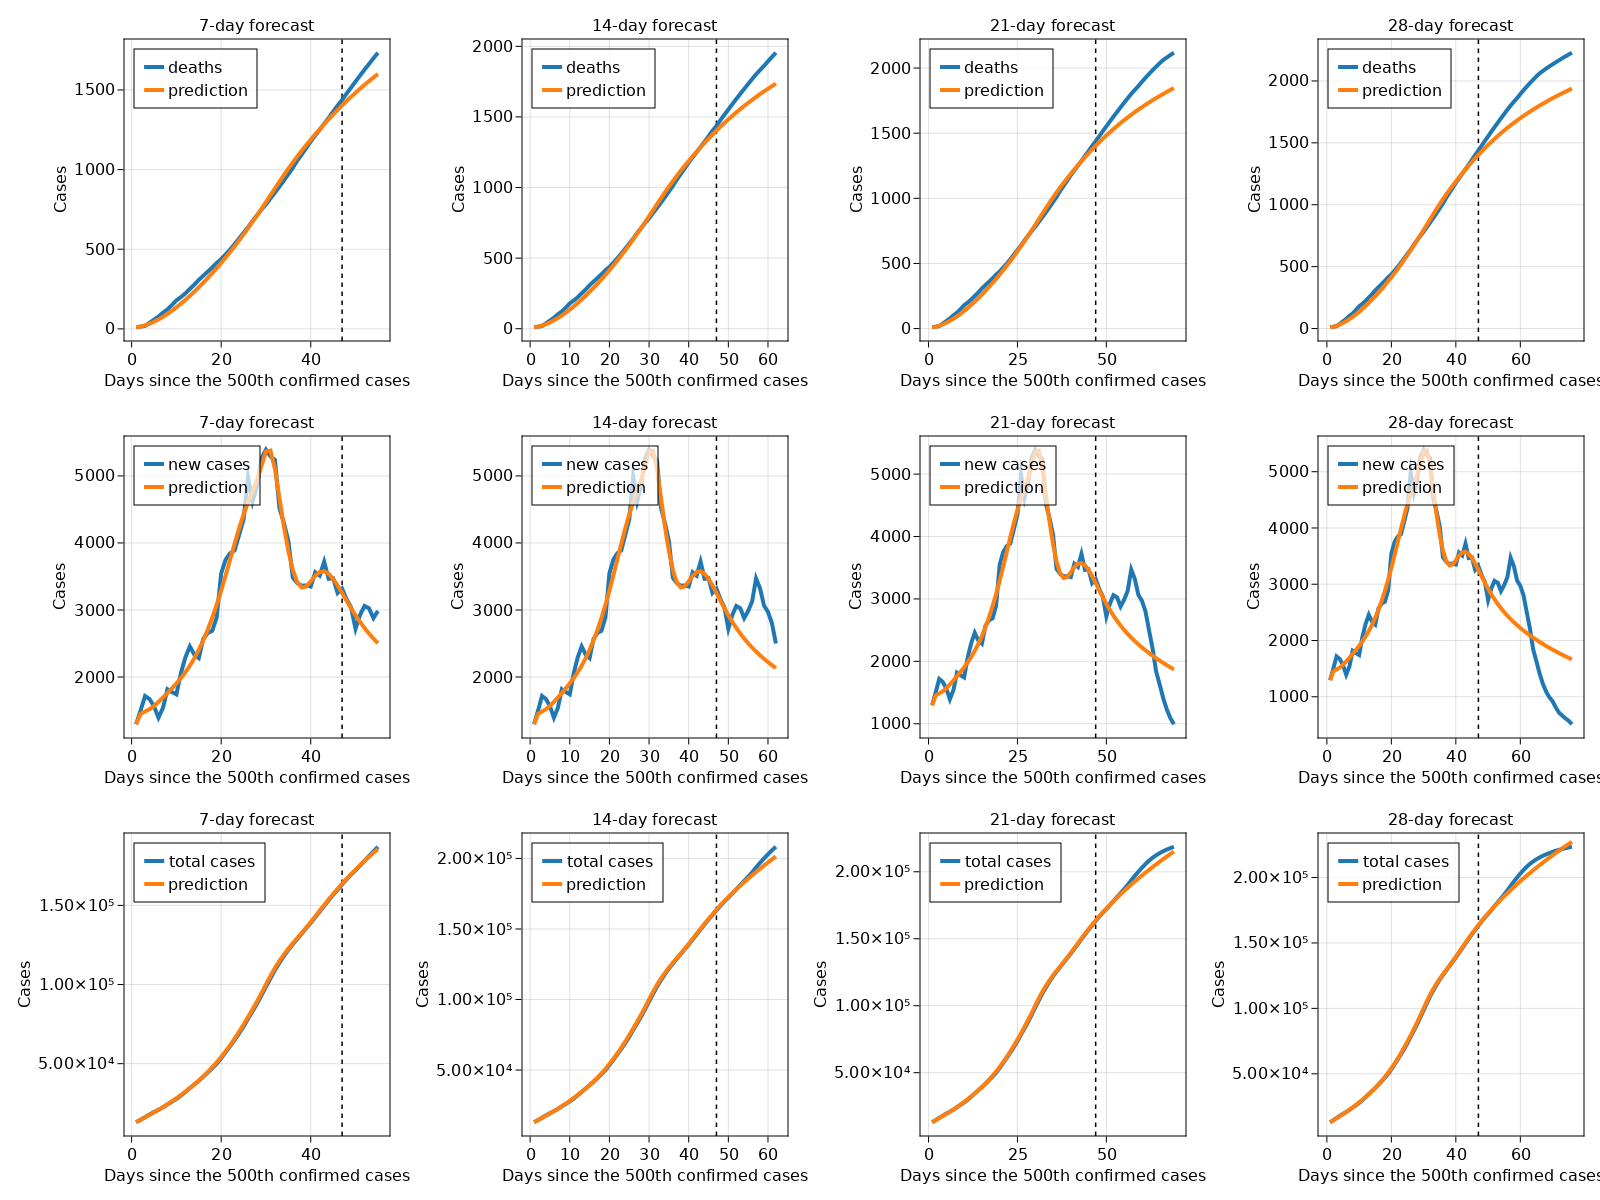
\includegraphics[scale=0.25]{baseline/binhduong/20211216111951.baseline.binhduong.forecasts.png}
    \caption{Predictions made by the baseline model after having trained with data for Binh Duong. The black vertical dashed line marks the last day in the training period.}
    \label{fig:predictions-binhduong-baseline}
\end{figure}

\begin{figure}[!htb]
    \centering
    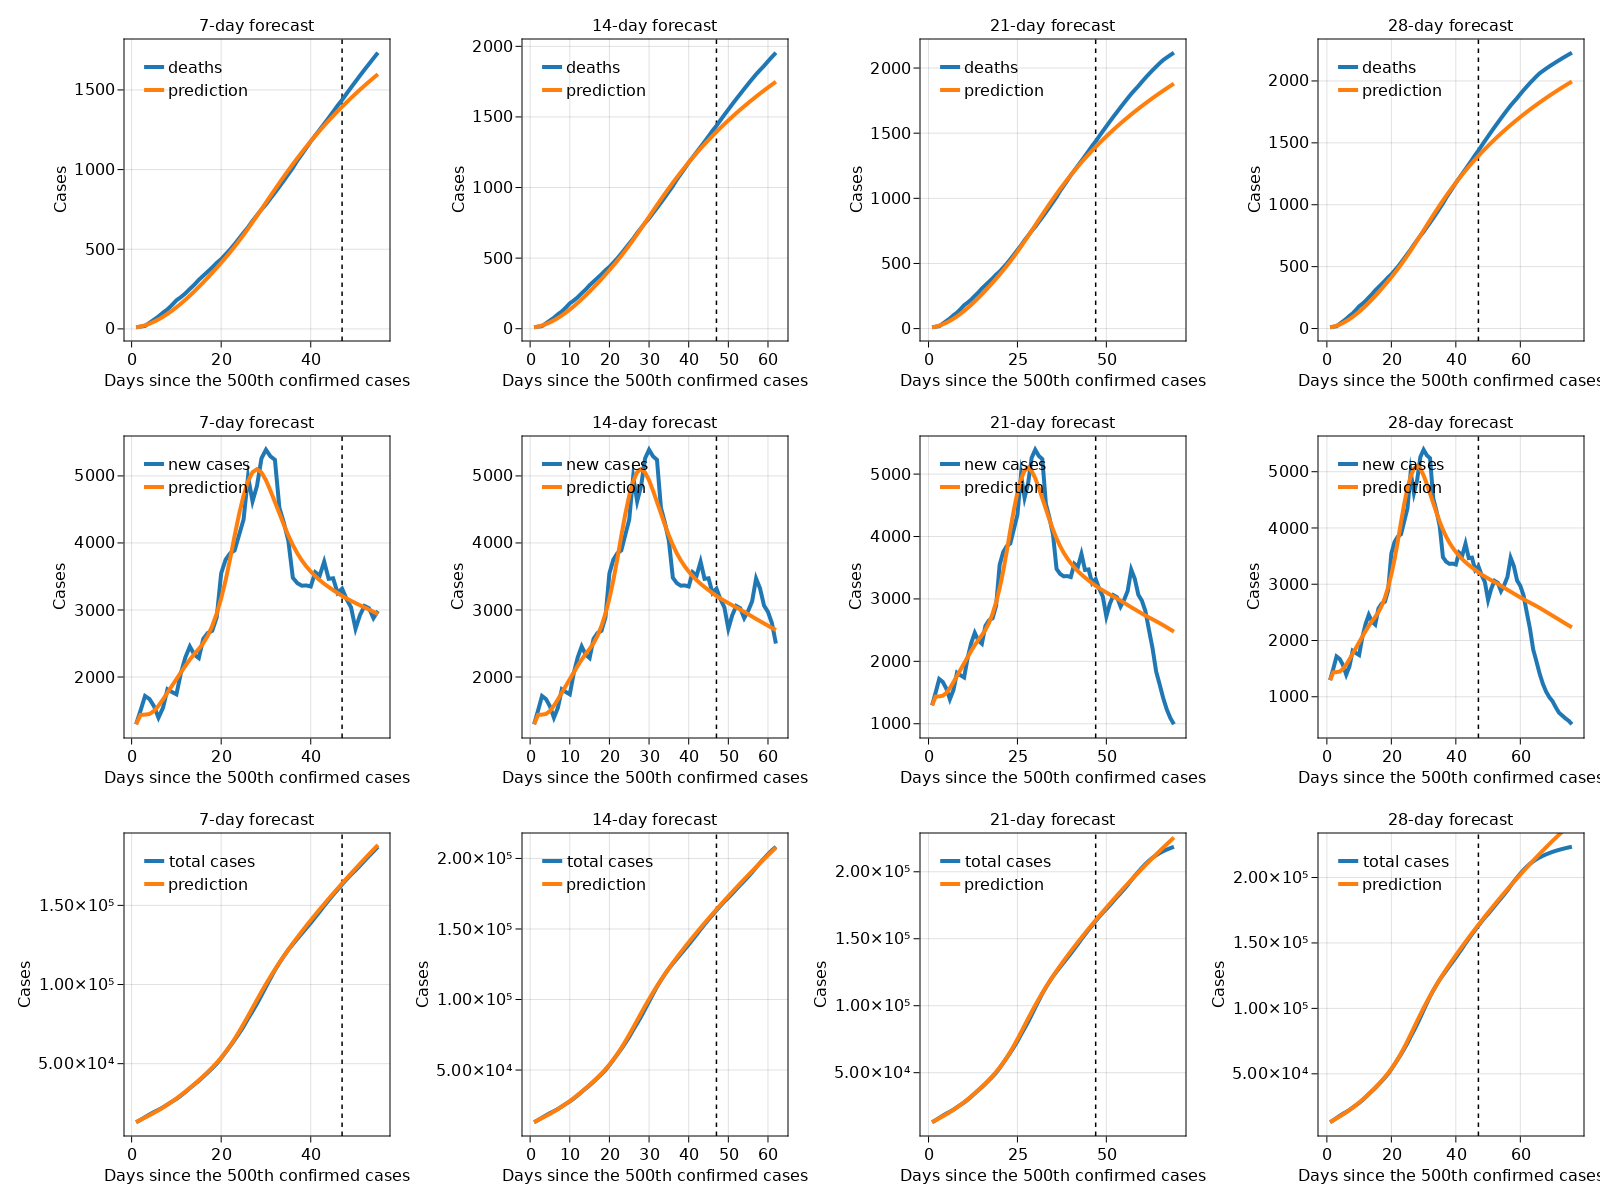
\includegraphics[scale=0.25]{fb1/binhduong/20211216173307.fbmobility1.binhduong.forecasts.png}
    \caption{Predictions made by the second version of the model that uses Facebook's Movement Range Maps dataset after having trained with data for Binh Duong. The black vertical dashed line marks the last day in the training period.}
    \label{fig:predictions-binhduong-fb1}
\end{figure}

\begin{figure}[!htb]
    \centering
    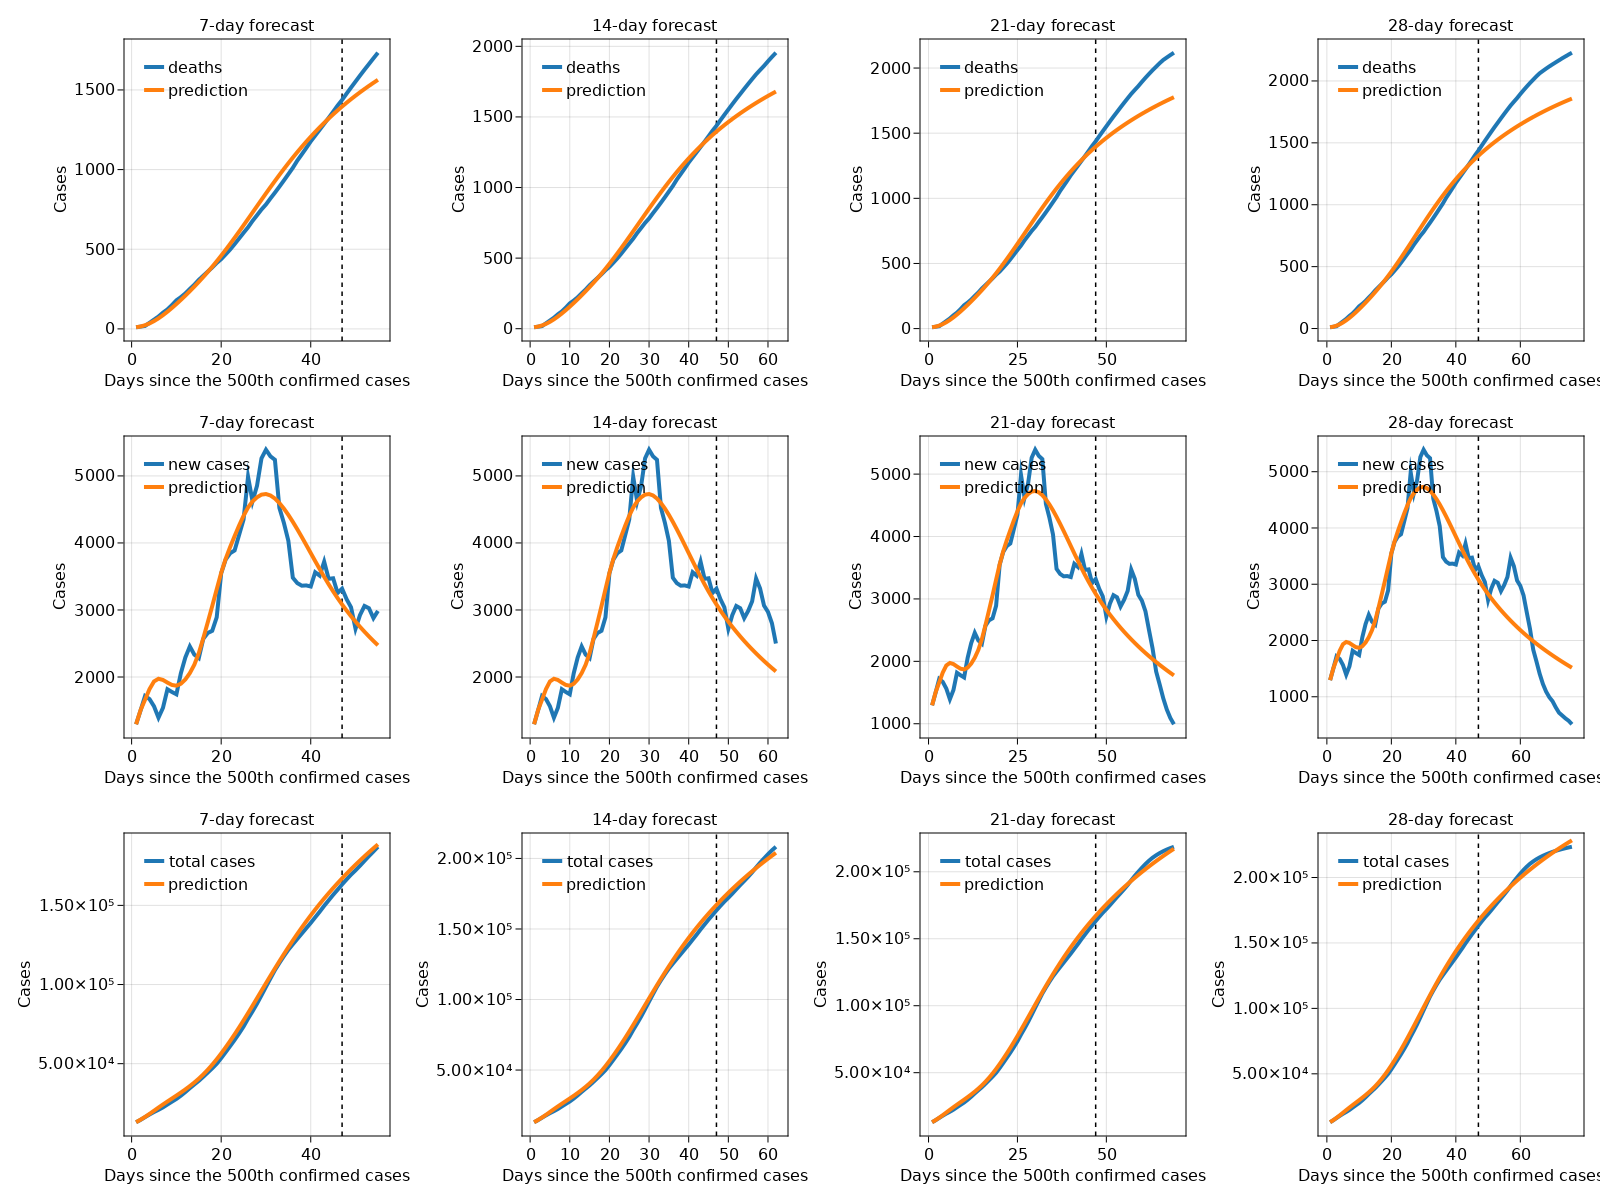
\includegraphics[scale=0.25]{fb2/binhduong/20211216172741.fbmobility2.binhduong.forecasts.png}
    \caption{Predictions made by the second version of the model that uses Facebook's Movement Range Maps dataset and Social Proximity to Cases Index after having trained with data for Binh duong. The black vertical dashed line marks the last day in the training period.}
    \label{fig:predictions-binhduong-fb2}
\end{figure}

% DONG NAI

\begin{figure}[!htb]
    \centering
    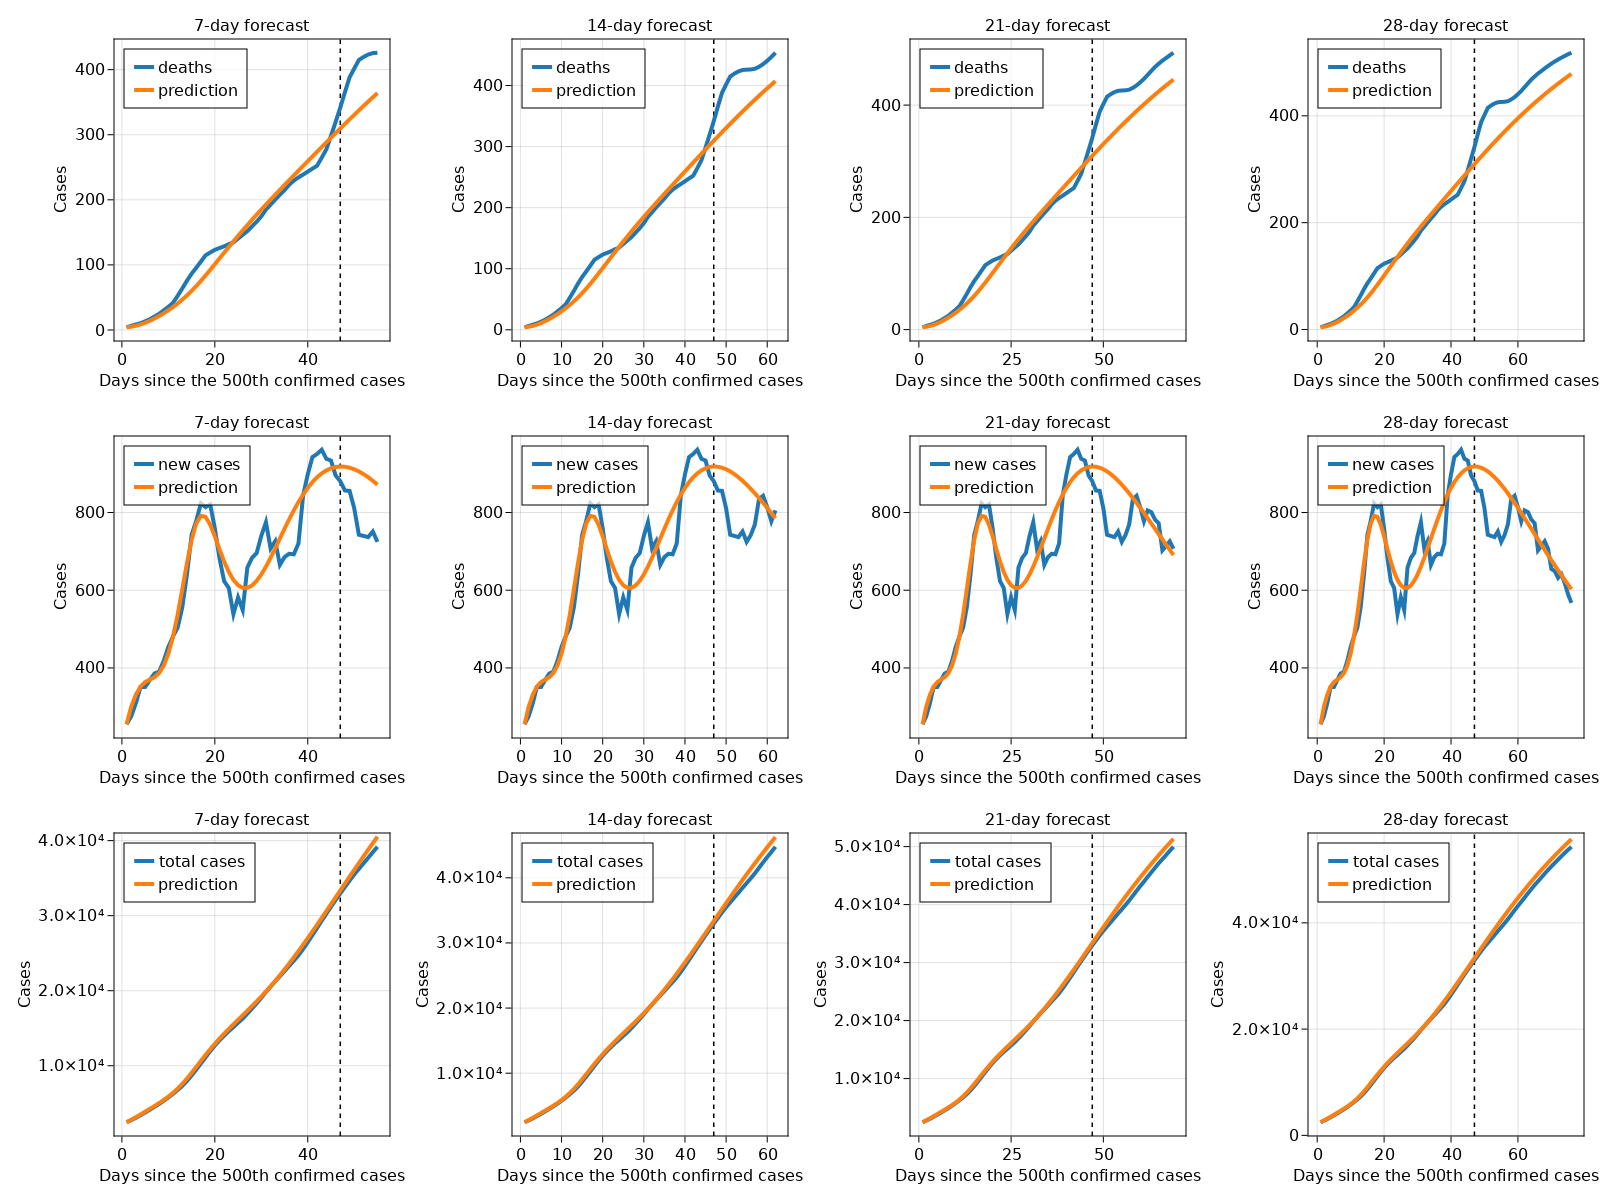
\includegraphics[scale=0.25]{baseline/dongnai/20211216211601.baseline.dongnai.forecasts.png}
    \caption{Predictions made by the baseline model after having trained with data for Dong Nai. The black vertical dashed line marks the last day in the training period.}
    \label{fig:predictions-dongnai-baseline}
\end{figure}

\begin{figure}[!htb]
    \centering
    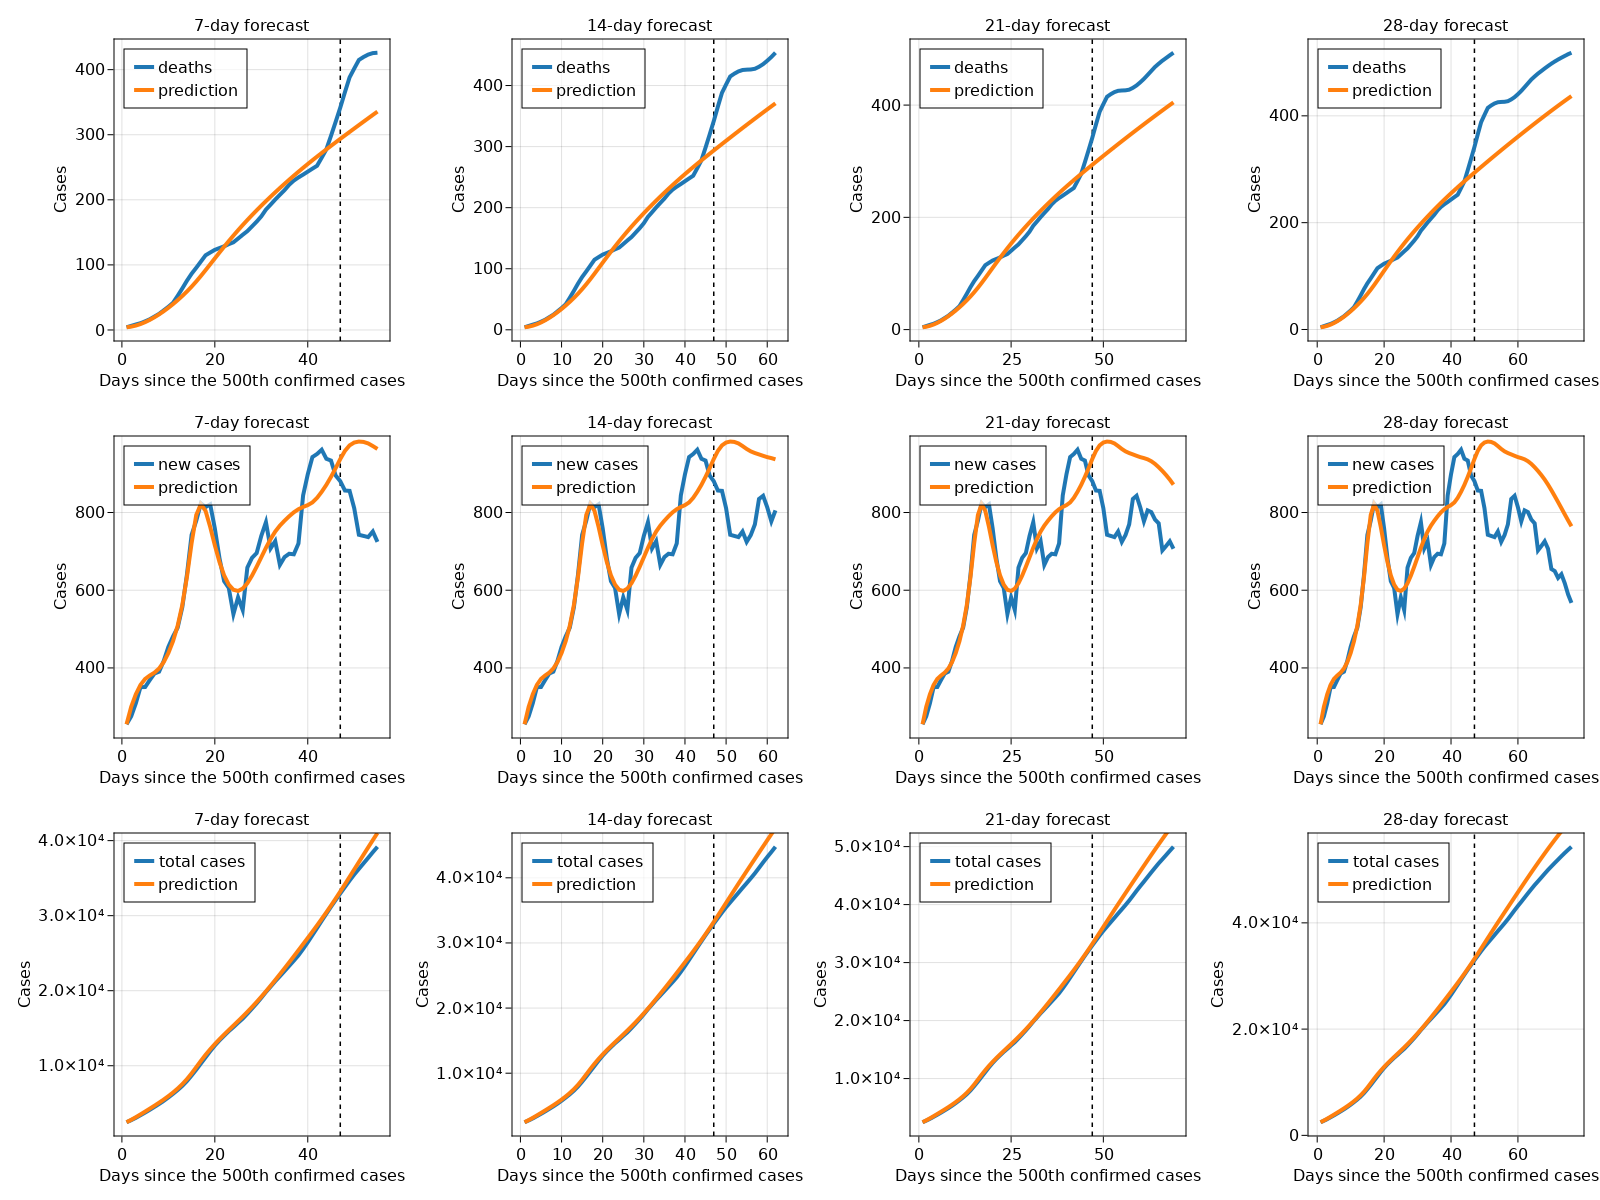
\includegraphics[scale=0.25]{fb1/dongnai/20211216131821.fbmobility1.dongnai.forecasts.png}
    \caption{Predictions made by the second version of the model that uses Facebook's Movement Range Maps dataset after having trained with data for Dong Nai. The black vertical dashed line marks the last day in the training period.}
    \label{fig:predictions-dongnai-fb1}
\end{figure}

\begin{figure}[!htb]
    \centering
    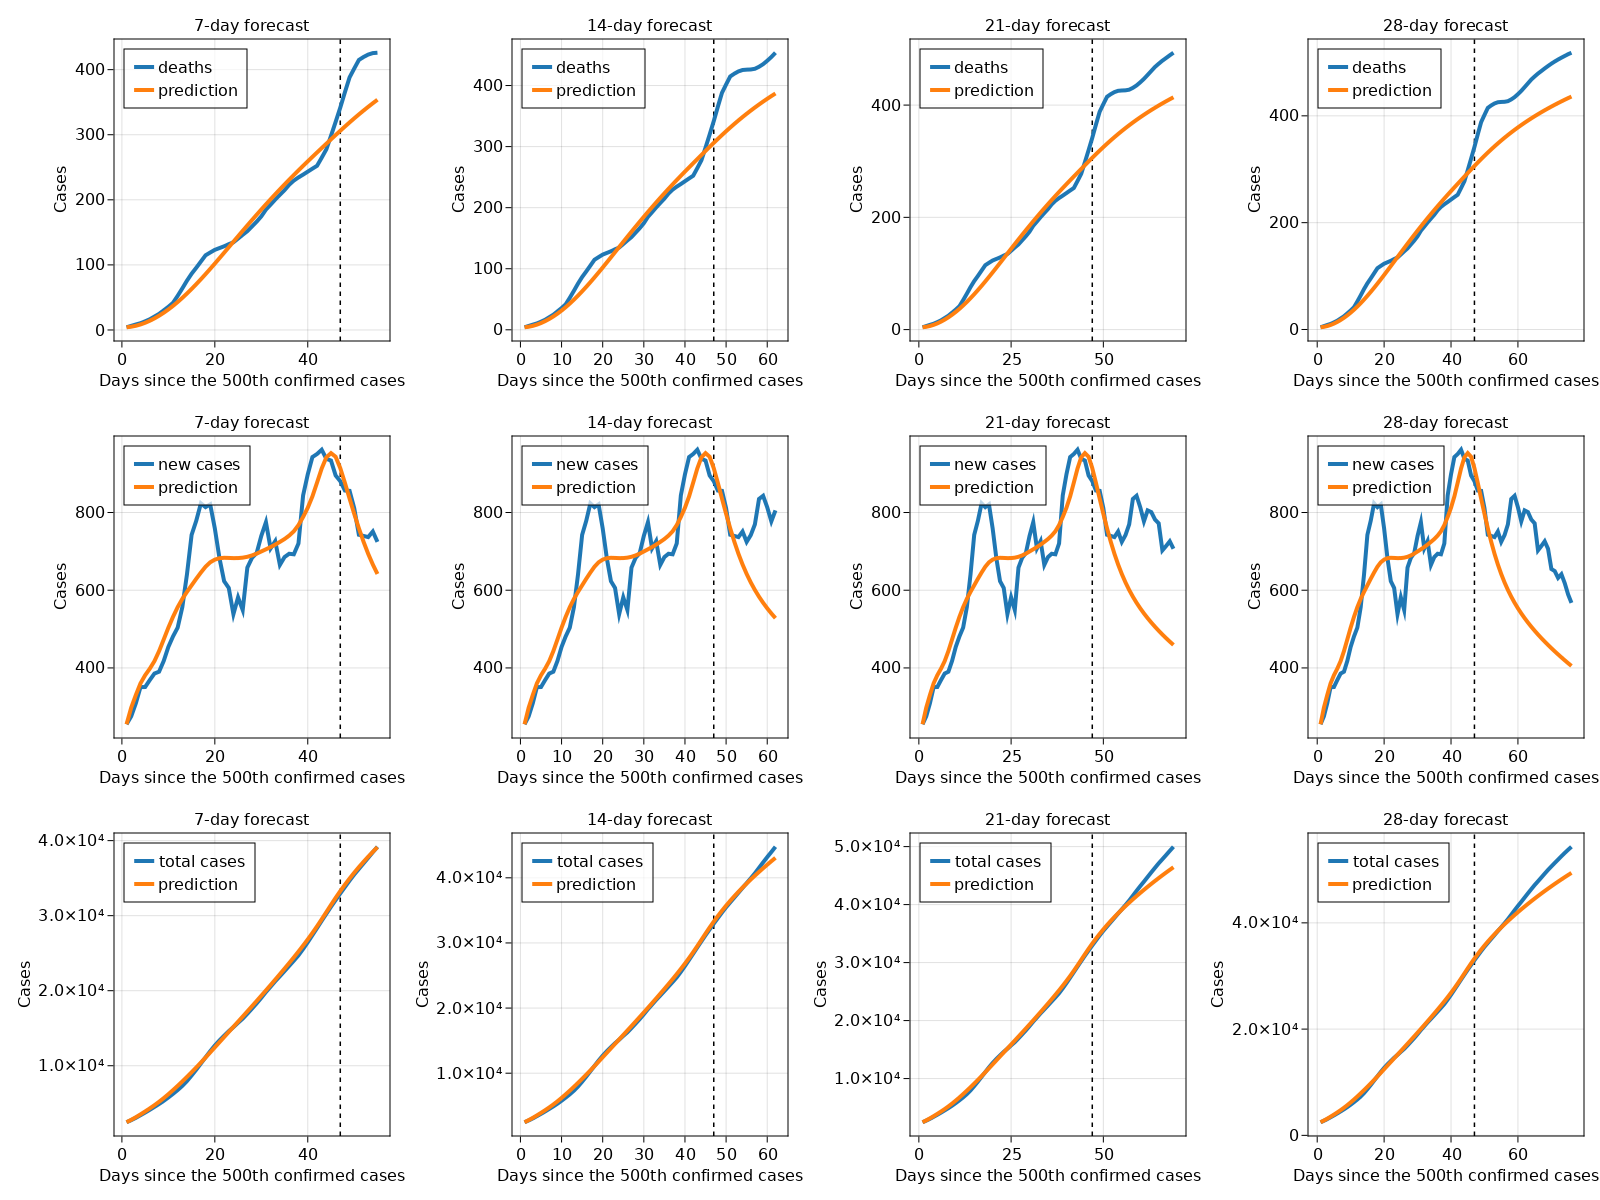
\includegraphics[scale=0.25]{fb2/dongnai/20211217220549.fbmobility2.dongnai.forecasts.png}
    \caption{Predictions made by the second version of the model that uses Facebook's Movement Range Maps dataset and Social Proximity to Cases Index after having trained with data for Dong Nai. The black vertical dashed line marks the last day in the training period.}
    \label{fig:predictions-dongnai-fb2}
\end{figure}

% HO CHI MINH CITY

\begin{figure}[!htb]
    \centering
    \includegraphics[scale=0.25]{baseline/hcm/20211216154445.baseline.hcm.forecasts.png}
    \caption{Predictions made by the baseline model after having trained with data for Ho Chi Minh city. The black vertical dashed line marks the last day in the training period.}
    \label{fig:predictions-hcm-baseline}
\end{figure}

\begin{figure}[!htb]
    \centering
    \includegraphics[scale=0.25]{fb1/hcm/20211216231719.fbmobility1.hcm.forecasts.png}
    \caption{Predictions made by the second version of the model that uses Facebook's Movement Range Maps dataset after having trained with data for Ho Chi Minh city. The black vertical dashed line marks the last day in the training period.}
    \label{fig:predictions-hcm-fb1}
\end{figure}

\begin{figure}[!htb]
    \centering
    \includegraphics[scale=0.25]{fb2/hcm/20211216183635.fbmobility2.hcm.forecasts.png}
    \caption{Predictions made by the second version of the model that uses Facebook's Movement Range Maps dataset and Social Proximity to Cases Index after having trained with data for Ho Chi Minh city. The black vertical dashed line marks the last day in the training period.}
    \label{fig:predictions-hcm-fb2}
\end{figure}

% LONG AN

\begin{figure}[!htb]
    \centering
    \includegraphics[scale=0.25]{baseline/longan/20211216111951.baseline.longan.forecasts.png}
    \caption{Predictions made by the baseline model after having trained with data for Long An. The black vertical dashed line marks the last day in the training period.}
    \label{fig:predictions-longan-baseline}
\end{figure}

\begin{figure}[!htb]
    \centering
    \includegraphics[scale=0.25]{fb1/longan/20211216131821.fbmobility1.longan.forecasts.png}
    \caption{Predictions made by the second version of the model that uses Facebook's Movement Range Maps dataset after having trained with data for Long An. The black vertical dashed line marks the last day in the training period.}
    \label{fig:predictions-longan-fb1}
\end{figure}

\begin{figure}[!htb]
    \centering
    \includegraphics[scale=0.25]{fb2/longan/20211216193717.fbmobility2.longan.forecasts.png}
    \caption{Predictions made by the second version of the model that uses Facebook's Movement Range Maps dataset and Social Proximity to Cases Index after having trained with data for Long An. The black vertical dashed line marks the last day in the training period.}
    \label{fig:predictions-longan-fb2}
\end{figure}

% ======== RESULTS ========
\appendix

\chapter{Model predictions}

% VIETNAM

\begin{figure}[!htb]
    \centering
    \includegraphics[scale=0.25]{baseline/vietnam/20211216111951.baseline.vietnam.forecasts.png}
    \caption{Predictions made by the baseline model after having trained with data for Vietnam. The black vertical dashed line marks the last day in the training period.}
    \label{fig:predictions-vietnam-baseline}
\end{figure}

\begin{figure}[!htb]
    \centering
    \includegraphics[scale=0.25]{fb1/vietnam/20211216231719.fbmobility1.vietnam.forecasts.png}
    \caption{Predictions made by the second version of the model that uses Facebook's Movement Range Maps dataset after having trained with data for Vietnam. The black vertical dashed line marks the last day in the training period.}
    \label{fig:predictions-vietnam-fb1}
\end{figure}

% US

\begin{figure}[!htb]
    \centering
    \includegraphics[scale=0.25]{baseline/unitedstates/20211216125000.baseline.unitedstates.forecasts.png}
    \caption{Predictions made by the baseline model after having trained with data for the United States. The black vertical dashed line marks the last day in the training period.}
    \label{fig:predictions-usa-baseline}
\end{figure}

\begin{figure}[!htb]
    \centering
    \includegraphics[scale=0.25]{fb1/unitedstates/20211216233634.fbmobility1.unitedstates.forecasts.png}
    \caption{Predictions made by the second version of the model that uses Facebook's Movement Range Maps dataset after having trained with data for the United States. The black vertical dashed line marks the last day in the training period.}
    \label{fig:predictions-usa-fb1}
\end{figure}

% LOS ANGELES

\begin{figure}[!htb]
    \centering
    \includegraphics[scale=0.25]{baseline/losangeles_ca/20211216124108.baseline.losangeles_ca.forecasts.png}
    \caption{Predictions made by the baseline model after having trained with data for Los Angeles, California. The black vertical dashed line marks the last day in the training period.}
    \label{fig:predictions-losangeles-baseline}
\end{figure}

\begin{figure}[!htb]
    \centering
    \includegraphics[scale=0.25]{fb1/losangeles_ca/20211216180602.fbmobility1.losangeles_ca.forecasts.png}
    \caption{Predictions made by the second version of the model that uses Facebook's Movement Range Maps dataset after having trained with data for Los Angeles, California. The black vertical dashed line marks the last day in the training period.}
    \label{fig:predictions-losangeles-fb1}
\end{figure}

\begin{figure}[!htb]
    \centering
    \includegraphics[scale=0.25]{fb2/losangeles_ca/20211216142727.fbmobility2.losangeles_ca.forecasts.png}
    \caption{Predictions made by the second version of the model that uses Facebook's Movement Range Maps dataset and Social Proximity to Cases Index after having trained with data for Los Angeles, California. The black vertical dashed line marks the last day in the training period.}
    \label{fig:predictions-losangeles-fb2}
\end{figure}

% HARRIS

\begin{figure}[!htb]
    \centering
    \includegraphics[scale=0.25]{baseline/harris_tx/20211216154445.baseline.harris_tx.forecasts.png}
    \caption{Predictions made by the baseline model after having trained with data for Harris, Texas. The black vertical dashed line marks the last day in the training period.}
    \label{fig:predictions-harris-baseline}
\end{figure}

\begin{figure}[!htb]
    \centering
    \includegraphics[scale=0.25]{fb1/harris_tx/20211216231719.fbmobility1.harris_tx.forecasts.png}
    \caption{Predictions made by the second version of the model that uses Facebook's Movement Range Maps dataset after having trained with data for Harris, Texas. The black vertical dashed line marks the last day in the training period.}
    \label{fig:predictions-harris-fb1}
\end{figure}

\begin{figure}[!htb]
    \centering
    \includegraphics[scale=0.25]{fb2/harris_tx/20211217204936.fbmobility2.harris_tx.forecasts.png}
    \caption{Predictions made by the second version of the model that uses Facebook's Movement Range Maps dataset and Social Proximity to Cases Index after having trained with data for Harris, Texas. The black vertical dashed line marks the last day in the training period.}
    \label{fig:predictions-harris-fb2}
\end{figure}

% COOK

\begin{figure}[!htb]
    \centering
    \includegraphics[scale=0.25]{baseline/cook_il/20211215163025.baseline.cook_il.forecasts.png}
    \caption{Predictions made by the baseline model after having trained with data for Cook, Illinois. The black vertical dashed line marks the last day in the training period.}
    \label{fig:predictions-cook-baseline}
\end{figure}

\begin{figure}[!htb]
    \centering
    \includegraphics[scale=0.25]{fb1/cook_il/20211216131821.fbmobility1.cook_il.forecasts.png}
    \caption{Predictions made by the second version of the model that uses Facebook's Movement Range Maps dataset after having trained with data for Cook, Illinois. The black vertical dashed line marks the last day in the training period.}
    \label{fig:predictions-cook-fb1}
\end{figure}

\begin{figure}[!htb]
    \centering
    \includegraphics[scale=0.25]{fb2/cook_il/20211216142727.fbmobility2.cook_il.forecasts.png}
    \caption{Predictions made by the second version of the model that uses Facebook's Movement Range Maps dataset and Social Proximity to Cases Index after having trained with data for Cook, Illinois. The black vertical dashed line marks the last day in the training period.}
    \label{fig:predictions-cook-fb2}
\end{figure}

% MARICOPA

\begin{figure}[!htb]
    \centering
    \includegraphics[scale=0.25]{fb1/cook_il/20211216131821.fbmobility1.cook_il.forecasts.png}
    \caption{Predictions made by the baseline model after having trained with data for Maricopa, Arizona. The black vertical dashed line marks the last day in the training period.}
    \label{fig:predictions-maricopa-baseline}
\end{figure}

\begin{figure}[!htb]
    \centering
    \includegraphics[scale=0.25]{fb1/maricopa_az/20211216131821.fbmobility1.maricopa_az.forecasts.png}
    \caption{Predictions made by the second version of the model that uses Facebook's Movement Range Maps dataset after having trained with data for Maricopa, Arizona. The black vertical dashed line marks the last day in the training period.}
    \label{fig:predictions-maricopa-fb1}
\end{figure}

\begin{figure}[!htb]
    \centering
    \includegraphics[scale=0.25]{fb2/maricopa_az/20211216193717.fbmobility2.maricopa_az.forecasts.png}
    \caption{Predictions made by the second version of the model that uses Facebook's Movement Range Maps dataset and Social Proximity to Cases Index after having trained with data for Maricopa, Arizona. The black vertical dashed line marks the last day in the training period.}
    \label{fig:predictions-maricopa-fb2}
\end{figure}

% BINH DUONG

\begin{figure}[!htb]
    \centering
    \includegraphics[scale=0.25]{baseline/binhduong/20211216111951.baseline.binhduong.forecasts.png}
    \caption{Predictions made by the baseline model after having trained with data for Binh Duong. The black vertical dashed line marks the last day in the training period.}
    \label{fig:predictions-binhduong-baseline}
\end{figure}

\begin{figure}[!htb]
    \centering
    \includegraphics[scale=0.25]{fb1/binhduong/20211216173307.fbmobility1.binhduong.forecasts.png}
    \caption{Predictions made by the second version of the model that uses Facebook's Movement Range Maps dataset after having trained with data for Binh Duong. The black vertical dashed line marks the last day in the training period.}
    \label{fig:predictions-binhduong-fb1}
\end{figure}

\begin{figure}[!htb]
    \centering
    \includegraphics[scale=0.25]{fb2/binhduong/20211216172741.fbmobility2.binhduong.forecasts.png}
    \caption{Predictions made by the second version of the model that uses Facebook's Movement Range Maps dataset and Social Proximity to Cases Index after having trained with data for Binh duong. The black vertical dashed line marks the last day in the training period.}
    \label{fig:predictions-binhduong-fb2}
\end{figure}

% DONG NAI

\begin{figure}[!htb]
    \centering
    \includegraphics[scale=0.25]{baseline/dongnai/20211216211601.baseline.dongnai.forecasts.png}
    \caption{Predictions made by the baseline model after having trained with data for Dong Nai. The black vertical dashed line marks the last day in the training period.}
    \label{fig:predictions-dongnai-baseline}
\end{figure}

\begin{figure}[!htb]
    \centering
    \includegraphics[scale=0.25]{fb1/dongnai/20211216131821.fbmobility1.dongnai.forecasts.png}
    \caption{Predictions made by the second version of the model that uses Facebook's Movement Range Maps dataset after having trained with data for Dong Nai. The black vertical dashed line marks the last day in the training period.}
    \label{fig:predictions-dongnai-fb1}
\end{figure}

\begin{figure}[!htb]
    \centering
    \includegraphics[scale=0.25]{fb2/dongnai/20211217220549.fbmobility2.dongnai.forecasts.png}
    \caption{Predictions made by the second version of the model that uses Facebook's Movement Range Maps dataset and Social Proximity to Cases Index after having trained with data for Dong Nai. The black vertical dashed line marks the last day in the training period.}
    \label{fig:predictions-dongnai-fb2}
\end{figure}

% HO CHI MINH CITY

\begin{figure}[!htb]
    \centering
    \includegraphics[scale=0.25]{baseline/hcm/20211216154445.baseline.hcm.forecasts.png}
    \caption{Predictions made by the baseline model after having trained with data for Ho Chi Minh city. The black vertical dashed line marks the last day in the training period.}
    \label{fig:predictions-hcm-baseline}
\end{figure}

\begin{figure}[!htb]
    \centering
    \includegraphics[scale=0.25]{fb1/hcm/20211216231719.fbmobility1.hcm.forecasts.png}
    \caption{Predictions made by the second version of the model that uses Facebook's Movement Range Maps dataset after having trained with data for Ho Chi Minh city. The black vertical dashed line marks the last day in the training period.}
    \label{fig:predictions-hcm-fb1}
\end{figure}

\begin{figure}[!htb]
    \centering
    \includegraphics[scale=0.25]{fb2/hcm/20211216183635.fbmobility2.hcm.forecasts.png}
    \caption{Predictions made by the second version of the model that uses Facebook's Movement Range Maps dataset and Social Proximity to Cases Index after having trained with data for Ho Chi Minh city. The black vertical dashed line marks the last day in the training period.}
    \label{fig:predictions-hcm-fb2}
\end{figure}

% LONG AN

\begin{figure}[!htb]
    \centering
    \includegraphics[scale=0.25]{baseline/longan/20211216111951.baseline.longan.forecasts.png}
    \caption{Predictions made by the baseline model after having trained with data for Long An. The black vertical dashed line marks the last day in the training period.}
    \label{fig:predictions-longan-baseline}
\end{figure}

\begin{figure}[!htb]
    \centering
    \includegraphics[scale=0.25]{fb1/longan/20211216131821.fbmobility1.longan.forecasts.png}
    \caption{Predictions made by the second version of the model that uses Facebook's Movement Range Maps dataset after having trained with data for Long An. The black vertical dashed line marks the last day in the training period.}
    \label{fig:predictions-longan-fb1}
\end{figure}

\begin{figure}[!htb]
    \centering
    \includegraphics[scale=0.25]{fb2/longan/20211216193717.fbmobility2.longan.forecasts.png}
    \caption{Predictions made by the second version of the model that uses Facebook's Movement Range Maps dataset and Social Proximity to Cases Index after having trained with data for Long An. The black vertical dashed line marks the last day in the training period.}
    \label{fig:predictions-longan-fb2}
\end{figure}

% ======== RESULTS ========
\appendix

\chapter{Model predictions}

% VIETNAM

\begin{figure}[!htb]
    \centering
    \includegraphics[scale=0.25]{baseline/vietnam/20211216111951.baseline.vietnam.forecasts.png}
    \caption{Predictions made by the baseline model after having trained with data for Vietnam. The black vertical dashed line marks the last day in the training period.}
    \label{fig:predictions-vietnam-baseline}
\end{figure}

\begin{figure}[!htb]
    \centering
    \includegraphics[scale=0.25]{fb1/vietnam/20211216231719.fbmobility1.vietnam.forecasts.png}
    \caption{Predictions made by the second version of the model that uses Facebook's Movement Range Maps dataset after having trained with data for Vietnam. The black vertical dashed line marks the last day in the training period.}
    \label{fig:predictions-vietnam-fb1}
\end{figure}

% US

\begin{figure}[!htb]
    \centering
    \includegraphics[scale=0.25]{baseline/unitedstates/20211216125000.baseline.unitedstates.forecasts.png}
    \caption{Predictions made by the baseline model after having trained with data for the United States. The black vertical dashed line marks the last day in the training period.}
    \label{fig:predictions-usa-baseline}
\end{figure}

\begin{figure}[!htb]
    \centering
    \includegraphics[scale=0.25]{fb1/unitedstates/20211216233634.fbmobility1.unitedstates.forecasts.png}
    \caption{Predictions made by the second version of the model that uses Facebook's Movement Range Maps dataset after having trained with data for the United States. The black vertical dashed line marks the last day in the training period.}
    \label{fig:predictions-usa-fb1}
\end{figure}

% LOS ANGELES

\begin{figure}[!htb]
    \centering
    \includegraphics[scale=0.25]{baseline/losangeles_ca/20211216124108.baseline.losangeles_ca.forecasts.png}
    \caption{Predictions made by the baseline model after having trained with data for Los Angeles, California. The black vertical dashed line marks the last day in the training period.}
    \label{fig:predictions-losangeles-baseline}
\end{figure}

\begin{figure}[!htb]
    \centering
    \includegraphics[scale=0.25]{fb1/losangeles_ca/20211216180602.fbmobility1.losangeles_ca.forecasts.png}
    \caption{Predictions made by the second version of the model that uses Facebook's Movement Range Maps dataset after having trained with data for Los Angeles, California. The black vertical dashed line marks the last day in the training period.}
    \label{fig:predictions-losangeles-fb1}
\end{figure}

\begin{figure}[!htb]
    \centering
    \includegraphics[scale=0.25]{fb2/losangeles_ca/20211216142727.fbmobility2.losangeles_ca.forecasts.png}
    \caption{Predictions made by the second version of the model that uses Facebook's Movement Range Maps dataset and Social Proximity to Cases Index after having trained with data for Los Angeles, California. The black vertical dashed line marks the last day in the training period.}
    \label{fig:predictions-losangeles-fb2}
\end{figure}

% HARRIS

\begin{figure}[!htb]
    \centering
    \includegraphics[scale=0.25]{baseline/harris_tx/20211216154445.baseline.harris_tx.forecasts.png}
    \caption{Predictions made by the baseline model after having trained with data for Harris, Texas. The black vertical dashed line marks the last day in the training period.}
    \label{fig:predictions-harris-baseline}
\end{figure}

\begin{figure}[!htb]
    \centering
    \includegraphics[scale=0.25]{fb1/harris_tx/20211216231719.fbmobility1.harris_tx.forecasts.png}
    \caption{Predictions made by the second version of the model that uses Facebook's Movement Range Maps dataset after having trained with data for Harris, Texas. The black vertical dashed line marks the last day in the training period.}
    \label{fig:predictions-harris-fb1}
\end{figure}

\begin{figure}[!htb]
    \centering
    \includegraphics[scale=0.25]{fb2/harris_tx/20211217204936.fbmobility2.harris_tx.forecasts.png}
    \caption{Predictions made by the second version of the model that uses Facebook's Movement Range Maps dataset and Social Proximity to Cases Index after having trained with data for Harris, Texas. The black vertical dashed line marks the last day in the training period.}
    \label{fig:predictions-harris-fb2}
\end{figure}

% COOK

\begin{figure}[!htb]
    \centering
    \includegraphics[scale=0.25]{baseline/cook_il/20211215163025.baseline.cook_il.forecasts.png}
    \caption{Predictions made by the baseline model after having trained with data for Cook, Illinois. The black vertical dashed line marks the last day in the training period.}
    \label{fig:predictions-cook-baseline}
\end{figure}

\begin{figure}[!htb]
    \centering
    \includegraphics[scale=0.25]{fb1/cook_il/20211216131821.fbmobility1.cook_il.forecasts.png}
    \caption{Predictions made by the second version of the model that uses Facebook's Movement Range Maps dataset after having trained with data for Cook, Illinois. The black vertical dashed line marks the last day in the training period.}
    \label{fig:predictions-cook-fb1}
\end{figure}

\begin{figure}[!htb]
    \centering
    \includegraphics[scale=0.25]{fb2/cook_il/20211216142727.fbmobility2.cook_il.forecasts.png}
    \caption{Predictions made by the second version of the model that uses Facebook's Movement Range Maps dataset and Social Proximity to Cases Index after having trained with data for Cook, Illinois. The black vertical dashed line marks the last day in the training period.}
    \label{fig:predictions-cook-fb2}
\end{figure}

% MARICOPA

\begin{figure}[!htb]
    \centering
    \includegraphics[scale=0.25]{fb1/cook_il/20211216131821.fbmobility1.cook_il.forecasts.png}
    \caption{Predictions made by the baseline model after having trained with data for Maricopa, Arizona. The black vertical dashed line marks the last day in the training period.}
    \label{fig:predictions-maricopa-baseline}
\end{figure}

\begin{figure}[!htb]
    \centering
    \includegraphics[scale=0.25]{fb1/maricopa_az/20211216131821.fbmobility1.maricopa_az.forecasts.png}
    \caption{Predictions made by the second version of the model that uses Facebook's Movement Range Maps dataset after having trained with data for Maricopa, Arizona. The black vertical dashed line marks the last day in the training period.}
    \label{fig:predictions-maricopa-fb1}
\end{figure}

\begin{figure}[!htb]
    \centering
    \includegraphics[scale=0.25]{fb2/maricopa_az/20211216193717.fbmobility2.maricopa_az.forecasts.png}
    \caption{Predictions made by the second version of the model that uses Facebook's Movement Range Maps dataset and Social Proximity to Cases Index after having trained with data for Maricopa, Arizona. The black vertical dashed line marks the last day in the training period.}
    \label{fig:predictions-maricopa-fb2}
\end{figure}

% BINH DUONG

\begin{figure}[!htb]
    \centering
    \includegraphics[scale=0.25]{baseline/binhduong/20211216111951.baseline.binhduong.forecasts.png}
    \caption{Predictions made by the baseline model after having trained with data for Binh Duong. The black vertical dashed line marks the last day in the training period.}
    \label{fig:predictions-binhduong-baseline}
\end{figure}

\begin{figure}[!htb]
    \centering
    \includegraphics[scale=0.25]{fb1/binhduong/20211216173307.fbmobility1.binhduong.forecasts.png}
    \caption{Predictions made by the second version of the model that uses Facebook's Movement Range Maps dataset after having trained with data for Binh Duong. The black vertical dashed line marks the last day in the training period.}
    \label{fig:predictions-binhduong-fb1}
\end{figure}

\begin{figure}[!htb]
    \centering
    \includegraphics[scale=0.25]{fb2/binhduong/20211216172741.fbmobility2.binhduong.forecasts.png}
    \caption{Predictions made by the second version of the model that uses Facebook's Movement Range Maps dataset and Social Proximity to Cases Index after having trained with data for Binh duong. The black vertical dashed line marks the last day in the training period.}
    \label{fig:predictions-binhduong-fb2}
\end{figure}

% DONG NAI

\begin{figure}[!htb]
    \centering
    \includegraphics[scale=0.25]{baseline/dongnai/20211216211601.baseline.dongnai.forecasts.png}
    \caption{Predictions made by the baseline model after having trained with data for Dong Nai. The black vertical dashed line marks the last day in the training period.}
    \label{fig:predictions-dongnai-baseline}
\end{figure}

\begin{figure}[!htb]
    \centering
    \includegraphics[scale=0.25]{fb1/dongnai/20211216131821.fbmobility1.dongnai.forecasts.png}
    \caption{Predictions made by the second version of the model that uses Facebook's Movement Range Maps dataset after having trained with data for Dong Nai. The black vertical dashed line marks the last day in the training period.}
    \label{fig:predictions-dongnai-fb1}
\end{figure}

\begin{figure}[!htb]
    \centering
    \includegraphics[scale=0.25]{fb2/dongnai/20211217220549.fbmobility2.dongnai.forecasts.png}
    \caption{Predictions made by the second version of the model that uses Facebook's Movement Range Maps dataset and Social Proximity to Cases Index after having trained with data for Dong Nai. The black vertical dashed line marks the last day in the training period.}
    \label{fig:predictions-dongnai-fb2}
\end{figure}

% HO CHI MINH CITY

\begin{figure}[!htb]
    \centering
    \includegraphics[scale=0.25]{baseline/hcm/20211216154445.baseline.hcm.forecasts.png}
    \caption{Predictions made by the baseline model after having trained with data for Ho Chi Minh city. The black vertical dashed line marks the last day in the training period.}
    \label{fig:predictions-hcm-baseline}
\end{figure}

\begin{figure}[!htb]
    \centering
    \includegraphics[scale=0.25]{fb1/hcm/20211216231719.fbmobility1.hcm.forecasts.png}
    \caption{Predictions made by the second version of the model that uses Facebook's Movement Range Maps dataset after having trained with data for Ho Chi Minh city. The black vertical dashed line marks the last day in the training period.}
    \label{fig:predictions-hcm-fb1}
\end{figure}

\begin{figure}[!htb]
    \centering
    \includegraphics[scale=0.25]{fb2/hcm/20211216183635.fbmobility2.hcm.forecasts.png}
    \caption{Predictions made by the second version of the model that uses Facebook's Movement Range Maps dataset and Social Proximity to Cases Index after having trained with data for Ho Chi Minh city. The black vertical dashed line marks the last day in the training period.}
    \label{fig:predictions-hcm-fb2}
\end{figure}

% LONG AN

\begin{figure}[!htb]
    \centering
    \includegraphics[scale=0.25]{baseline/longan/20211216111951.baseline.longan.forecasts.png}
    \caption{Predictions made by the baseline model after having trained with data for Long An. The black vertical dashed line marks the last day in the training period.}
    \label{fig:predictions-longan-baseline}
\end{figure}

\begin{figure}[!htb]
    \centering
    \includegraphics[scale=0.25]{fb1/longan/20211216131821.fbmobility1.longan.forecasts.png}
    \caption{Predictions made by the second version of the model that uses Facebook's Movement Range Maps dataset after having trained with data for Long An. The black vertical dashed line marks the last day in the training period.}
    \label{fig:predictions-longan-fb1}
\end{figure}

\begin{figure}[!htb]
    \centering
    \includegraphics[scale=0.25]{fb2/longan/20211216193717.fbmobility2.longan.forecasts.png}
    \caption{Predictions made by the second version of the model that uses Facebook's Movement Range Maps dataset and Social Proximity to Cases Index after having trained with data for Long An. The black vertical dashed line marks the last day in the training period.}
    \label{fig:predictions-longan-fb2}
\end{figure}

% ======== DISCUSSION ========
\appendix

\chapter{Model predictions}

% VIETNAM

\begin{figure}[!htb]
    \centering
    \includegraphics[scale=0.25]{baseline/vietnam/20211216111951.baseline.vietnam.forecasts.png}
    \caption{Predictions made by the baseline model after having trained with data for Vietnam. The black vertical dashed line marks the last day in the training period.}
    \label{fig:predictions-vietnam-baseline}
\end{figure}

\begin{figure}[!htb]
    \centering
    \includegraphics[scale=0.25]{fb1/vietnam/20211216231719.fbmobility1.vietnam.forecasts.png}
    \caption{Predictions made by the second version of the model that uses Facebook's Movement Range Maps dataset after having trained with data for Vietnam. The black vertical dashed line marks the last day in the training period.}
    \label{fig:predictions-vietnam-fb1}
\end{figure}

% US

\begin{figure}[!htb]
    \centering
    \includegraphics[scale=0.25]{baseline/unitedstates/20211216125000.baseline.unitedstates.forecasts.png}
    \caption{Predictions made by the baseline model after having trained with data for the United States. The black vertical dashed line marks the last day in the training period.}
    \label{fig:predictions-usa-baseline}
\end{figure}

\begin{figure}[!htb]
    \centering
    \includegraphics[scale=0.25]{fb1/unitedstates/20211216233634.fbmobility1.unitedstates.forecasts.png}
    \caption{Predictions made by the second version of the model that uses Facebook's Movement Range Maps dataset after having trained with data for the United States. The black vertical dashed line marks the last day in the training period.}
    \label{fig:predictions-usa-fb1}
\end{figure}

% LOS ANGELES

\begin{figure}[!htb]
    \centering
    \includegraphics[scale=0.25]{baseline/losangeles_ca/20211216124108.baseline.losangeles_ca.forecasts.png}
    \caption{Predictions made by the baseline model after having trained with data for Los Angeles, California. The black vertical dashed line marks the last day in the training period.}
    \label{fig:predictions-losangeles-baseline}
\end{figure}

\begin{figure}[!htb]
    \centering
    \includegraphics[scale=0.25]{fb1/losangeles_ca/20211216180602.fbmobility1.losangeles_ca.forecasts.png}
    \caption{Predictions made by the second version of the model that uses Facebook's Movement Range Maps dataset after having trained with data for Los Angeles, California. The black vertical dashed line marks the last day in the training period.}
    \label{fig:predictions-losangeles-fb1}
\end{figure}

\begin{figure}[!htb]
    \centering
    \includegraphics[scale=0.25]{fb2/losangeles_ca/20211216142727.fbmobility2.losangeles_ca.forecasts.png}
    \caption{Predictions made by the second version of the model that uses Facebook's Movement Range Maps dataset and Social Proximity to Cases Index after having trained with data for Los Angeles, California. The black vertical dashed line marks the last day in the training period.}
    \label{fig:predictions-losangeles-fb2}
\end{figure}

% HARRIS

\begin{figure}[!htb]
    \centering
    \includegraphics[scale=0.25]{baseline/harris_tx/20211216154445.baseline.harris_tx.forecasts.png}
    \caption{Predictions made by the baseline model after having trained with data for Harris, Texas. The black vertical dashed line marks the last day in the training period.}
    \label{fig:predictions-harris-baseline}
\end{figure}

\begin{figure}[!htb]
    \centering
    \includegraphics[scale=0.25]{fb1/harris_tx/20211216231719.fbmobility1.harris_tx.forecasts.png}
    \caption{Predictions made by the second version of the model that uses Facebook's Movement Range Maps dataset after having trained with data for Harris, Texas. The black vertical dashed line marks the last day in the training period.}
    \label{fig:predictions-harris-fb1}
\end{figure}

\begin{figure}[!htb]
    \centering
    \includegraphics[scale=0.25]{fb2/harris_tx/20211217204936.fbmobility2.harris_tx.forecasts.png}
    \caption{Predictions made by the second version of the model that uses Facebook's Movement Range Maps dataset and Social Proximity to Cases Index after having trained with data for Harris, Texas. The black vertical dashed line marks the last day in the training period.}
    \label{fig:predictions-harris-fb2}
\end{figure}

% COOK

\begin{figure}[!htb]
    \centering
    \includegraphics[scale=0.25]{baseline/cook_il/20211215163025.baseline.cook_il.forecasts.png}
    \caption{Predictions made by the baseline model after having trained with data for Cook, Illinois. The black vertical dashed line marks the last day in the training period.}
    \label{fig:predictions-cook-baseline}
\end{figure}

\begin{figure}[!htb]
    \centering
    \includegraphics[scale=0.25]{fb1/cook_il/20211216131821.fbmobility1.cook_il.forecasts.png}
    \caption{Predictions made by the second version of the model that uses Facebook's Movement Range Maps dataset after having trained with data for Cook, Illinois. The black vertical dashed line marks the last day in the training period.}
    \label{fig:predictions-cook-fb1}
\end{figure}

\begin{figure}[!htb]
    \centering
    \includegraphics[scale=0.25]{fb2/cook_il/20211216142727.fbmobility2.cook_il.forecasts.png}
    \caption{Predictions made by the second version of the model that uses Facebook's Movement Range Maps dataset and Social Proximity to Cases Index after having trained with data for Cook, Illinois. The black vertical dashed line marks the last day in the training period.}
    \label{fig:predictions-cook-fb2}
\end{figure}

% MARICOPA

\begin{figure}[!htb]
    \centering
    \includegraphics[scale=0.25]{fb1/cook_il/20211216131821.fbmobility1.cook_il.forecasts.png}
    \caption{Predictions made by the baseline model after having trained with data for Maricopa, Arizona. The black vertical dashed line marks the last day in the training period.}
    \label{fig:predictions-maricopa-baseline}
\end{figure}

\begin{figure}[!htb]
    \centering
    \includegraphics[scale=0.25]{fb1/maricopa_az/20211216131821.fbmobility1.maricopa_az.forecasts.png}
    \caption{Predictions made by the second version of the model that uses Facebook's Movement Range Maps dataset after having trained with data for Maricopa, Arizona. The black vertical dashed line marks the last day in the training period.}
    \label{fig:predictions-maricopa-fb1}
\end{figure}

\begin{figure}[!htb]
    \centering
    \includegraphics[scale=0.25]{fb2/maricopa_az/20211216193717.fbmobility2.maricopa_az.forecasts.png}
    \caption{Predictions made by the second version of the model that uses Facebook's Movement Range Maps dataset and Social Proximity to Cases Index after having trained with data for Maricopa, Arizona. The black vertical dashed line marks the last day in the training period.}
    \label{fig:predictions-maricopa-fb2}
\end{figure}

% BINH DUONG

\begin{figure}[!htb]
    \centering
    \includegraphics[scale=0.25]{baseline/binhduong/20211216111951.baseline.binhduong.forecasts.png}
    \caption{Predictions made by the baseline model after having trained with data for Binh Duong. The black vertical dashed line marks the last day in the training period.}
    \label{fig:predictions-binhduong-baseline}
\end{figure}

\begin{figure}[!htb]
    \centering
    \includegraphics[scale=0.25]{fb1/binhduong/20211216173307.fbmobility1.binhduong.forecasts.png}
    \caption{Predictions made by the second version of the model that uses Facebook's Movement Range Maps dataset after having trained with data for Binh Duong. The black vertical dashed line marks the last day in the training period.}
    \label{fig:predictions-binhduong-fb1}
\end{figure}

\begin{figure}[!htb]
    \centering
    \includegraphics[scale=0.25]{fb2/binhduong/20211216172741.fbmobility2.binhduong.forecasts.png}
    \caption{Predictions made by the second version of the model that uses Facebook's Movement Range Maps dataset and Social Proximity to Cases Index after having trained with data for Binh duong. The black vertical dashed line marks the last day in the training period.}
    \label{fig:predictions-binhduong-fb2}
\end{figure}

% DONG NAI

\begin{figure}[!htb]
    \centering
    \includegraphics[scale=0.25]{baseline/dongnai/20211216211601.baseline.dongnai.forecasts.png}
    \caption{Predictions made by the baseline model after having trained with data for Dong Nai. The black vertical dashed line marks the last day in the training period.}
    \label{fig:predictions-dongnai-baseline}
\end{figure}

\begin{figure}[!htb]
    \centering
    \includegraphics[scale=0.25]{fb1/dongnai/20211216131821.fbmobility1.dongnai.forecasts.png}
    \caption{Predictions made by the second version of the model that uses Facebook's Movement Range Maps dataset after having trained with data for Dong Nai. The black vertical dashed line marks the last day in the training period.}
    \label{fig:predictions-dongnai-fb1}
\end{figure}

\begin{figure}[!htb]
    \centering
    \includegraphics[scale=0.25]{fb2/dongnai/20211217220549.fbmobility2.dongnai.forecasts.png}
    \caption{Predictions made by the second version of the model that uses Facebook's Movement Range Maps dataset and Social Proximity to Cases Index after having trained with data for Dong Nai. The black vertical dashed line marks the last day in the training period.}
    \label{fig:predictions-dongnai-fb2}
\end{figure}

% HO CHI MINH CITY

\begin{figure}[!htb]
    \centering
    \includegraphics[scale=0.25]{baseline/hcm/20211216154445.baseline.hcm.forecasts.png}
    \caption{Predictions made by the baseline model after having trained with data for Ho Chi Minh city. The black vertical dashed line marks the last day in the training period.}
    \label{fig:predictions-hcm-baseline}
\end{figure}

\begin{figure}[!htb]
    \centering
    \includegraphics[scale=0.25]{fb1/hcm/20211216231719.fbmobility1.hcm.forecasts.png}
    \caption{Predictions made by the second version of the model that uses Facebook's Movement Range Maps dataset after having trained with data for Ho Chi Minh city. The black vertical dashed line marks the last day in the training period.}
    \label{fig:predictions-hcm-fb1}
\end{figure}

\begin{figure}[!htb]
    \centering
    \includegraphics[scale=0.25]{fb2/hcm/20211216183635.fbmobility2.hcm.forecasts.png}
    \caption{Predictions made by the second version of the model that uses Facebook's Movement Range Maps dataset and Social Proximity to Cases Index after having trained with data for Ho Chi Minh city. The black vertical dashed line marks the last day in the training period.}
    \label{fig:predictions-hcm-fb2}
\end{figure}

% LONG AN

\begin{figure}[!htb]
    \centering
    \includegraphics[scale=0.25]{baseline/longan/20211216111951.baseline.longan.forecasts.png}
    \caption{Predictions made by the baseline model after having trained with data for Long An. The black vertical dashed line marks the last day in the training period.}
    \label{fig:predictions-longan-baseline}
\end{figure}

\begin{figure}[!htb]
    \centering
    \includegraphics[scale=0.25]{fb1/longan/20211216131821.fbmobility1.longan.forecasts.png}
    \caption{Predictions made by the second version of the model that uses Facebook's Movement Range Maps dataset after having trained with data for Long An. The black vertical dashed line marks the last day in the training period.}
    \label{fig:predictions-longan-fb1}
\end{figure}

\begin{figure}[!htb]
    \centering
    \includegraphics[scale=0.25]{fb2/longan/20211216193717.fbmobility2.longan.forecasts.png}
    \caption{Predictions made by the second version of the model that uses Facebook's Movement Range Maps dataset and Social Proximity to Cases Index after having trained with data for Long An. The black vertical dashed line marks the last day in the training period.}
    \label{fig:predictions-longan-fb2}
\end{figure}

% ======== CONCLUSION ========
\appendix

\chapter{Model predictions}

% VIETNAM

\begin{figure}[!htb]
    \centering
    \includegraphics[scale=0.25]{baseline/vietnam/20211216111951.baseline.vietnam.forecasts.png}
    \caption{Predictions made by the baseline model after having trained with data for Vietnam. The black vertical dashed line marks the last day in the training period.}
    \label{fig:predictions-vietnam-baseline}
\end{figure}

\begin{figure}[!htb]
    \centering
    \includegraphics[scale=0.25]{fb1/vietnam/20211216231719.fbmobility1.vietnam.forecasts.png}
    \caption{Predictions made by the second version of the model that uses Facebook's Movement Range Maps dataset after having trained with data for Vietnam. The black vertical dashed line marks the last day in the training period.}
    \label{fig:predictions-vietnam-fb1}
\end{figure}

% US

\begin{figure}[!htb]
    \centering
    \includegraphics[scale=0.25]{baseline/unitedstates/20211216125000.baseline.unitedstates.forecasts.png}
    \caption{Predictions made by the baseline model after having trained with data for the United States. The black vertical dashed line marks the last day in the training period.}
    \label{fig:predictions-usa-baseline}
\end{figure}

\begin{figure}[!htb]
    \centering
    \includegraphics[scale=0.25]{fb1/unitedstates/20211216233634.fbmobility1.unitedstates.forecasts.png}
    \caption{Predictions made by the second version of the model that uses Facebook's Movement Range Maps dataset after having trained with data for the United States. The black vertical dashed line marks the last day in the training period.}
    \label{fig:predictions-usa-fb1}
\end{figure}

% LOS ANGELES

\begin{figure}[!htb]
    \centering
    \includegraphics[scale=0.25]{baseline/losangeles_ca/20211216124108.baseline.losangeles_ca.forecasts.png}
    \caption{Predictions made by the baseline model after having trained with data for Los Angeles, California. The black vertical dashed line marks the last day in the training period.}
    \label{fig:predictions-losangeles-baseline}
\end{figure}

\begin{figure}[!htb]
    \centering
    \includegraphics[scale=0.25]{fb1/losangeles_ca/20211216180602.fbmobility1.losangeles_ca.forecasts.png}
    \caption{Predictions made by the second version of the model that uses Facebook's Movement Range Maps dataset after having trained with data for Los Angeles, California. The black vertical dashed line marks the last day in the training period.}
    \label{fig:predictions-losangeles-fb1}
\end{figure}

\begin{figure}[!htb]
    \centering
    \includegraphics[scale=0.25]{fb2/losangeles_ca/20211216142727.fbmobility2.losangeles_ca.forecasts.png}
    \caption{Predictions made by the second version of the model that uses Facebook's Movement Range Maps dataset and Social Proximity to Cases Index after having trained with data for Los Angeles, California. The black vertical dashed line marks the last day in the training period.}
    \label{fig:predictions-losangeles-fb2}
\end{figure}

% HARRIS

\begin{figure}[!htb]
    \centering
    \includegraphics[scale=0.25]{baseline/harris_tx/20211216154445.baseline.harris_tx.forecasts.png}
    \caption{Predictions made by the baseline model after having trained with data for Harris, Texas. The black vertical dashed line marks the last day in the training period.}
    \label{fig:predictions-harris-baseline}
\end{figure}

\begin{figure}[!htb]
    \centering
    \includegraphics[scale=0.25]{fb1/harris_tx/20211216231719.fbmobility1.harris_tx.forecasts.png}
    \caption{Predictions made by the second version of the model that uses Facebook's Movement Range Maps dataset after having trained with data for Harris, Texas. The black vertical dashed line marks the last day in the training period.}
    \label{fig:predictions-harris-fb1}
\end{figure}

\begin{figure}[!htb]
    \centering
    \includegraphics[scale=0.25]{fb2/harris_tx/20211217204936.fbmobility2.harris_tx.forecasts.png}
    \caption{Predictions made by the second version of the model that uses Facebook's Movement Range Maps dataset and Social Proximity to Cases Index after having trained with data for Harris, Texas. The black vertical dashed line marks the last day in the training period.}
    \label{fig:predictions-harris-fb2}
\end{figure}

% COOK

\begin{figure}[!htb]
    \centering
    \includegraphics[scale=0.25]{baseline/cook_il/20211215163025.baseline.cook_il.forecasts.png}
    \caption{Predictions made by the baseline model after having trained with data for Cook, Illinois. The black vertical dashed line marks the last day in the training period.}
    \label{fig:predictions-cook-baseline}
\end{figure}

\begin{figure}[!htb]
    \centering
    \includegraphics[scale=0.25]{fb1/cook_il/20211216131821.fbmobility1.cook_il.forecasts.png}
    \caption{Predictions made by the second version of the model that uses Facebook's Movement Range Maps dataset after having trained with data for Cook, Illinois. The black vertical dashed line marks the last day in the training period.}
    \label{fig:predictions-cook-fb1}
\end{figure}

\begin{figure}[!htb]
    \centering
    \includegraphics[scale=0.25]{fb2/cook_il/20211216142727.fbmobility2.cook_il.forecasts.png}
    \caption{Predictions made by the second version of the model that uses Facebook's Movement Range Maps dataset and Social Proximity to Cases Index after having trained with data for Cook, Illinois. The black vertical dashed line marks the last day in the training period.}
    \label{fig:predictions-cook-fb2}
\end{figure}

% MARICOPA

\begin{figure}[!htb]
    \centering
    \includegraphics[scale=0.25]{fb1/cook_il/20211216131821.fbmobility1.cook_il.forecasts.png}
    \caption{Predictions made by the baseline model after having trained with data for Maricopa, Arizona. The black vertical dashed line marks the last day in the training period.}
    \label{fig:predictions-maricopa-baseline}
\end{figure}

\begin{figure}[!htb]
    \centering
    \includegraphics[scale=0.25]{fb1/maricopa_az/20211216131821.fbmobility1.maricopa_az.forecasts.png}
    \caption{Predictions made by the second version of the model that uses Facebook's Movement Range Maps dataset after having trained with data for Maricopa, Arizona. The black vertical dashed line marks the last day in the training period.}
    \label{fig:predictions-maricopa-fb1}
\end{figure}

\begin{figure}[!htb]
    \centering
    \includegraphics[scale=0.25]{fb2/maricopa_az/20211216193717.fbmobility2.maricopa_az.forecasts.png}
    \caption{Predictions made by the second version of the model that uses Facebook's Movement Range Maps dataset and Social Proximity to Cases Index after having trained with data for Maricopa, Arizona. The black vertical dashed line marks the last day in the training period.}
    \label{fig:predictions-maricopa-fb2}
\end{figure}

% BINH DUONG

\begin{figure}[!htb]
    \centering
    \includegraphics[scale=0.25]{baseline/binhduong/20211216111951.baseline.binhduong.forecasts.png}
    \caption{Predictions made by the baseline model after having trained with data for Binh Duong. The black vertical dashed line marks the last day in the training period.}
    \label{fig:predictions-binhduong-baseline}
\end{figure}

\begin{figure}[!htb]
    \centering
    \includegraphics[scale=0.25]{fb1/binhduong/20211216173307.fbmobility1.binhduong.forecasts.png}
    \caption{Predictions made by the second version of the model that uses Facebook's Movement Range Maps dataset after having trained with data for Binh Duong. The black vertical dashed line marks the last day in the training period.}
    \label{fig:predictions-binhduong-fb1}
\end{figure}

\begin{figure}[!htb]
    \centering
    \includegraphics[scale=0.25]{fb2/binhduong/20211216172741.fbmobility2.binhduong.forecasts.png}
    \caption{Predictions made by the second version of the model that uses Facebook's Movement Range Maps dataset and Social Proximity to Cases Index after having trained with data for Binh duong. The black vertical dashed line marks the last day in the training period.}
    \label{fig:predictions-binhduong-fb2}
\end{figure}

% DONG NAI

\begin{figure}[!htb]
    \centering
    \includegraphics[scale=0.25]{baseline/dongnai/20211216211601.baseline.dongnai.forecasts.png}
    \caption{Predictions made by the baseline model after having trained with data for Dong Nai. The black vertical dashed line marks the last day in the training period.}
    \label{fig:predictions-dongnai-baseline}
\end{figure}

\begin{figure}[!htb]
    \centering
    \includegraphics[scale=0.25]{fb1/dongnai/20211216131821.fbmobility1.dongnai.forecasts.png}
    \caption{Predictions made by the second version of the model that uses Facebook's Movement Range Maps dataset after having trained with data for Dong Nai. The black vertical dashed line marks the last day in the training period.}
    \label{fig:predictions-dongnai-fb1}
\end{figure}

\begin{figure}[!htb]
    \centering
    \includegraphics[scale=0.25]{fb2/dongnai/20211217220549.fbmobility2.dongnai.forecasts.png}
    \caption{Predictions made by the second version of the model that uses Facebook's Movement Range Maps dataset and Social Proximity to Cases Index after having trained with data for Dong Nai. The black vertical dashed line marks the last day in the training period.}
    \label{fig:predictions-dongnai-fb2}
\end{figure}

% HO CHI MINH CITY

\begin{figure}[!htb]
    \centering
    \includegraphics[scale=0.25]{baseline/hcm/20211216154445.baseline.hcm.forecasts.png}
    \caption{Predictions made by the baseline model after having trained with data for Ho Chi Minh city. The black vertical dashed line marks the last day in the training period.}
    \label{fig:predictions-hcm-baseline}
\end{figure}

\begin{figure}[!htb]
    \centering
    \includegraphics[scale=0.25]{fb1/hcm/20211216231719.fbmobility1.hcm.forecasts.png}
    \caption{Predictions made by the second version of the model that uses Facebook's Movement Range Maps dataset after having trained with data for Ho Chi Minh city. The black vertical dashed line marks the last day in the training period.}
    \label{fig:predictions-hcm-fb1}
\end{figure}

\begin{figure}[!htb]
    \centering
    \includegraphics[scale=0.25]{fb2/hcm/20211216183635.fbmobility2.hcm.forecasts.png}
    \caption{Predictions made by the second version of the model that uses Facebook's Movement Range Maps dataset and Social Proximity to Cases Index after having trained with data for Ho Chi Minh city. The black vertical dashed line marks the last day in the training period.}
    \label{fig:predictions-hcm-fb2}
\end{figure}

% LONG AN

\begin{figure}[!htb]
    \centering
    \includegraphics[scale=0.25]{baseline/longan/20211216111951.baseline.longan.forecasts.png}
    \caption{Predictions made by the baseline model after having trained with data for Long An. The black vertical dashed line marks the last day in the training period.}
    \label{fig:predictions-longan-baseline}
\end{figure}

\begin{figure}[!htb]
    \centering
    \includegraphics[scale=0.25]{fb1/longan/20211216131821.fbmobility1.longan.forecasts.png}
    \caption{Predictions made by the second version of the model that uses Facebook's Movement Range Maps dataset after having trained with data for Long An. The black vertical dashed line marks the last day in the training period.}
    \label{fig:predictions-longan-fb1}
\end{figure}

\begin{figure}[!htb]
    \centering
    \includegraphics[scale=0.25]{fb2/longan/20211216193717.fbmobility2.longan.forecasts.png}
    \caption{Predictions made by the second version of the model that uses Facebook's Movement Range Maps dataset and Social Proximity to Cases Index after having trained with data for Long An. The black vertical dashed line marks the last day in the training period.}
    \label{fig:predictions-longan-fb2}
\end{figure}

% ======== REFERENCES ========
\printbibliography[title=References]

% ======== REFERENCES ========
\appendix

\chapter{Model predictions}

% VIETNAM

\begin{figure}[!htb]
    \centering
    \includegraphics[scale=0.25]{baseline/vietnam/20211216111951.baseline.vietnam.forecasts.png}
    \caption{Predictions made by the baseline model after having trained with data for Vietnam. The black vertical dashed line marks the last day in the training period.}
    \label{fig:predictions-vietnam-baseline}
\end{figure}

\begin{figure}[!htb]
    \centering
    \includegraphics[scale=0.25]{fb1/vietnam/20211216231719.fbmobility1.vietnam.forecasts.png}
    \caption{Predictions made by the second version of the model that uses Facebook's Movement Range Maps dataset after having trained with data for Vietnam. The black vertical dashed line marks the last day in the training period.}
    \label{fig:predictions-vietnam-fb1}
\end{figure}

% US

\begin{figure}[!htb]
    \centering
    \includegraphics[scale=0.25]{baseline/unitedstates/20211216125000.baseline.unitedstates.forecasts.png}
    \caption{Predictions made by the baseline model after having trained with data for the United States. The black vertical dashed line marks the last day in the training period.}
    \label{fig:predictions-usa-baseline}
\end{figure}

\begin{figure}[!htb]
    \centering
    \includegraphics[scale=0.25]{fb1/unitedstates/20211216233634.fbmobility1.unitedstates.forecasts.png}
    \caption{Predictions made by the second version of the model that uses Facebook's Movement Range Maps dataset after having trained with data for the United States. The black vertical dashed line marks the last day in the training period.}
    \label{fig:predictions-usa-fb1}
\end{figure}

% LOS ANGELES

\begin{figure}[!htb]
    \centering
    \includegraphics[scale=0.25]{baseline/losangeles_ca/20211216124108.baseline.losangeles_ca.forecasts.png}
    \caption{Predictions made by the baseline model after having trained with data for Los Angeles, California. The black vertical dashed line marks the last day in the training period.}
    \label{fig:predictions-losangeles-baseline}
\end{figure}

\begin{figure}[!htb]
    \centering
    \includegraphics[scale=0.25]{fb1/losangeles_ca/20211216180602.fbmobility1.losangeles_ca.forecasts.png}
    \caption{Predictions made by the second version of the model that uses Facebook's Movement Range Maps dataset after having trained with data for Los Angeles, California. The black vertical dashed line marks the last day in the training period.}
    \label{fig:predictions-losangeles-fb1}
\end{figure}

\begin{figure}[!htb]
    \centering
    \includegraphics[scale=0.25]{fb2/losangeles_ca/20211216142727.fbmobility2.losangeles_ca.forecasts.png}
    \caption{Predictions made by the second version of the model that uses Facebook's Movement Range Maps dataset and Social Proximity to Cases Index after having trained with data for Los Angeles, California. The black vertical dashed line marks the last day in the training period.}
    \label{fig:predictions-losangeles-fb2}
\end{figure}

% HARRIS

\begin{figure}[!htb]
    \centering
    \includegraphics[scale=0.25]{baseline/harris_tx/20211216154445.baseline.harris_tx.forecasts.png}
    \caption{Predictions made by the baseline model after having trained with data for Harris, Texas. The black vertical dashed line marks the last day in the training period.}
    \label{fig:predictions-harris-baseline}
\end{figure}

\begin{figure}[!htb]
    \centering
    \includegraphics[scale=0.25]{fb1/harris_tx/20211216231719.fbmobility1.harris_tx.forecasts.png}
    \caption{Predictions made by the second version of the model that uses Facebook's Movement Range Maps dataset after having trained with data for Harris, Texas. The black vertical dashed line marks the last day in the training period.}
    \label{fig:predictions-harris-fb1}
\end{figure}

\begin{figure}[!htb]
    \centering
    \includegraphics[scale=0.25]{fb2/harris_tx/20211217204936.fbmobility2.harris_tx.forecasts.png}
    \caption{Predictions made by the second version of the model that uses Facebook's Movement Range Maps dataset and Social Proximity to Cases Index after having trained with data for Harris, Texas. The black vertical dashed line marks the last day in the training period.}
    \label{fig:predictions-harris-fb2}
\end{figure}

% COOK

\begin{figure}[!htb]
    \centering
    \includegraphics[scale=0.25]{baseline/cook_il/20211215163025.baseline.cook_il.forecasts.png}
    \caption{Predictions made by the baseline model after having trained with data for Cook, Illinois. The black vertical dashed line marks the last day in the training period.}
    \label{fig:predictions-cook-baseline}
\end{figure}

\begin{figure}[!htb]
    \centering
    \includegraphics[scale=0.25]{fb1/cook_il/20211216131821.fbmobility1.cook_il.forecasts.png}
    \caption{Predictions made by the second version of the model that uses Facebook's Movement Range Maps dataset after having trained with data for Cook, Illinois. The black vertical dashed line marks the last day in the training period.}
    \label{fig:predictions-cook-fb1}
\end{figure}

\begin{figure}[!htb]
    \centering
    \includegraphics[scale=0.25]{fb2/cook_il/20211216142727.fbmobility2.cook_il.forecasts.png}
    \caption{Predictions made by the second version of the model that uses Facebook's Movement Range Maps dataset and Social Proximity to Cases Index after having trained with data for Cook, Illinois. The black vertical dashed line marks the last day in the training period.}
    \label{fig:predictions-cook-fb2}
\end{figure}

% MARICOPA

\begin{figure}[!htb]
    \centering
    \includegraphics[scale=0.25]{fb1/cook_il/20211216131821.fbmobility1.cook_il.forecasts.png}
    \caption{Predictions made by the baseline model after having trained with data for Maricopa, Arizona. The black vertical dashed line marks the last day in the training period.}
    \label{fig:predictions-maricopa-baseline}
\end{figure}

\begin{figure}[!htb]
    \centering
    \includegraphics[scale=0.25]{fb1/maricopa_az/20211216131821.fbmobility1.maricopa_az.forecasts.png}
    \caption{Predictions made by the second version of the model that uses Facebook's Movement Range Maps dataset after having trained with data for Maricopa, Arizona. The black vertical dashed line marks the last day in the training period.}
    \label{fig:predictions-maricopa-fb1}
\end{figure}

\begin{figure}[!htb]
    \centering
    \includegraphics[scale=0.25]{fb2/maricopa_az/20211216193717.fbmobility2.maricopa_az.forecasts.png}
    \caption{Predictions made by the second version of the model that uses Facebook's Movement Range Maps dataset and Social Proximity to Cases Index after having trained with data for Maricopa, Arizona. The black vertical dashed line marks the last day in the training period.}
    \label{fig:predictions-maricopa-fb2}
\end{figure}

% BINH DUONG

\begin{figure}[!htb]
    \centering
    \includegraphics[scale=0.25]{baseline/binhduong/20211216111951.baseline.binhduong.forecasts.png}
    \caption{Predictions made by the baseline model after having trained with data for Binh Duong. The black vertical dashed line marks the last day in the training period.}
    \label{fig:predictions-binhduong-baseline}
\end{figure}

\begin{figure}[!htb]
    \centering
    \includegraphics[scale=0.25]{fb1/binhduong/20211216173307.fbmobility1.binhduong.forecasts.png}
    \caption{Predictions made by the second version of the model that uses Facebook's Movement Range Maps dataset after having trained with data for Binh Duong. The black vertical dashed line marks the last day in the training period.}
    \label{fig:predictions-binhduong-fb1}
\end{figure}

\begin{figure}[!htb]
    \centering
    \includegraphics[scale=0.25]{fb2/binhduong/20211216172741.fbmobility2.binhduong.forecasts.png}
    \caption{Predictions made by the second version of the model that uses Facebook's Movement Range Maps dataset and Social Proximity to Cases Index after having trained with data for Binh duong. The black vertical dashed line marks the last day in the training period.}
    \label{fig:predictions-binhduong-fb2}
\end{figure}

% DONG NAI

\begin{figure}[!htb]
    \centering
    \includegraphics[scale=0.25]{baseline/dongnai/20211216211601.baseline.dongnai.forecasts.png}
    \caption{Predictions made by the baseline model after having trained with data for Dong Nai. The black vertical dashed line marks the last day in the training period.}
    \label{fig:predictions-dongnai-baseline}
\end{figure}

\begin{figure}[!htb]
    \centering
    \includegraphics[scale=0.25]{fb1/dongnai/20211216131821.fbmobility1.dongnai.forecasts.png}
    \caption{Predictions made by the second version of the model that uses Facebook's Movement Range Maps dataset after having trained with data for Dong Nai. The black vertical dashed line marks the last day in the training period.}
    \label{fig:predictions-dongnai-fb1}
\end{figure}

\begin{figure}[!htb]
    \centering
    \includegraphics[scale=0.25]{fb2/dongnai/20211217220549.fbmobility2.dongnai.forecasts.png}
    \caption{Predictions made by the second version of the model that uses Facebook's Movement Range Maps dataset and Social Proximity to Cases Index after having trained with data for Dong Nai. The black vertical dashed line marks the last day in the training period.}
    \label{fig:predictions-dongnai-fb2}
\end{figure}

% HO CHI MINH CITY

\begin{figure}[!htb]
    \centering
    \includegraphics[scale=0.25]{baseline/hcm/20211216154445.baseline.hcm.forecasts.png}
    \caption{Predictions made by the baseline model after having trained with data for Ho Chi Minh city. The black vertical dashed line marks the last day in the training period.}
    \label{fig:predictions-hcm-baseline}
\end{figure}

\begin{figure}[!htb]
    \centering
    \includegraphics[scale=0.25]{fb1/hcm/20211216231719.fbmobility1.hcm.forecasts.png}
    \caption{Predictions made by the second version of the model that uses Facebook's Movement Range Maps dataset after having trained with data for Ho Chi Minh city. The black vertical dashed line marks the last day in the training period.}
    \label{fig:predictions-hcm-fb1}
\end{figure}

\begin{figure}[!htb]
    \centering
    \includegraphics[scale=0.25]{fb2/hcm/20211216183635.fbmobility2.hcm.forecasts.png}
    \caption{Predictions made by the second version of the model that uses Facebook's Movement Range Maps dataset and Social Proximity to Cases Index after having trained with data for Ho Chi Minh city. The black vertical dashed line marks the last day in the training period.}
    \label{fig:predictions-hcm-fb2}
\end{figure}

% LONG AN

\begin{figure}[!htb]
    \centering
    \includegraphics[scale=0.25]{baseline/longan/20211216111951.baseline.longan.forecasts.png}
    \caption{Predictions made by the baseline model after having trained with data for Long An. The black vertical dashed line marks the last day in the training period.}
    \label{fig:predictions-longan-baseline}
\end{figure}

\begin{figure}[!htb]
    \centering
    \includegraphics[scale=0.25]{fb1/longan/20211216131821.fbmobility1.longan.forecasts.png}
    \caption{Predictions made by the second version of the model that uses Facebook's Movement Range Maps dataset after having trained with data for Long An. The black vertical dashed line marks the last day in the training period.}
    \label{fig:predictions-longan-fb1}
\end{figure}

\begin{figure}[!htb]
    \centering
    \includegraphics[scale=0.25]{fb2/longan/20211216193717.fbmobility2.longan.forecasts.png}
    \caption{Predictions made by the second version of the model that uses Facebook's Movement Range Maps dataset and Social Proximity to Cases Index after having trained with data for Long An. The black vertical dashed line marks the last day in the training period.}
    \label{fig:predictions-longan-fb2}
\end{figure}

% ======== GLOSSARY ========
\printglossaries

\end{document}
